\documentclass[10pt, conference, a4paper, final]{IEEEtran}
\IEEEoverridecommandlockouts
% For better handling of math expressions
\usepackage{amsmath}

\usepackage[margin=1in]{geometry} % Adjust margins as needed
\usepackage{lipsum} % Provides sample text. Remove this for your actual document.
\usepackage{algorithm}
\usepackage{algorithmicx}
\usepackage{booktabs}

% For better formatting of lists
\usepackage{enumitem}
\usepackage{amssymb}
% Optional for improved typography
\usepackage{microtype}
\usepackage[margin=1in]{geometry} % Adjust margins as needed
\usepackage{lipsum} % Provides sample text. Remove this for your actual document.
\usepackage[table,xcdraw]{xcolor}
\usepackage{colortbl}
\usepackage{graphicx} % Required for including images
\usepackage{graphicx}
\usepackage{textcomp}
\usepackage{xcolor}
\usepackage{float}
\usepackage{amsmath}
\usepackage{longtable}
\usepackage{booktabs}
\usepackage{multicol}
\usepackage{multirow}
\usepackage{relsize, fullpage, url, array}
\usepackage{lscape, afterpage}
\usepackage{float,lscape}

\usepackage{amsmath}
\usepackage{mathtools}
\usepackage{tabularx}

\usepackage{graphicx}
\usepackage{textcomp}
\usepackage{xcolor}
\usepackage{subcaption}

\title{Pixel-Level Robustness Testing in Deep Learning: A Comparative Analysis of Adversarial and Normal Inputs}
\author{Arooj Arif}
\date{\today} % You can also specify a date manually

\begin{document}

\maketitle % This command creates the title


\begin{abstract}    
    
    This paper delves into the critical challenge of adversarial perturbations in deep learning models, emphasizing the paramount importance of model reliability and transparency in high-stakes scenarios. Our research specifically targets four distinct adversarial attacks, scrutinizing their varied impacts on model robustness and the models' responses to diverse perturbation intensities. By employing the SHAP (SHapley Additive exPlanations) Deep Explainer, our study meticulously dissects adversarial strategies at the pixel level, thereby unraveling the nuanced ways attackers manipulate model perception. The pixel-based analysis undertaken is pivotal, not only for validating our models' responses to adversarial interference but also for comprehending the inherent vulnerabilities that such attacks exploit. Our investigation also evaluates how various data traits influence model accuracy, providing a comprehensive understanding of factors affecting model robustness. Through the application of a t-test, our research robustly validates the influential significance of identified pixels, thereby cementing their critical role in fortifying deep learning models against digital threats. The outcomes of this study significantly enhance the interpretability and defense capabilities of deep learning models. While our initial findings stem from experiments on the MNIST dataset, the methodologies and insights we present bear far-reaching implications across various domains. Our research stands as a pivotal contribution towards fortifying deep learning models against the dynamically evolving landscape of digital threats, thus ensuring their enduring reliability in both present and future technological landscapes.


\end{abstract}
\begin{figure*}[!ht]
    \centering
    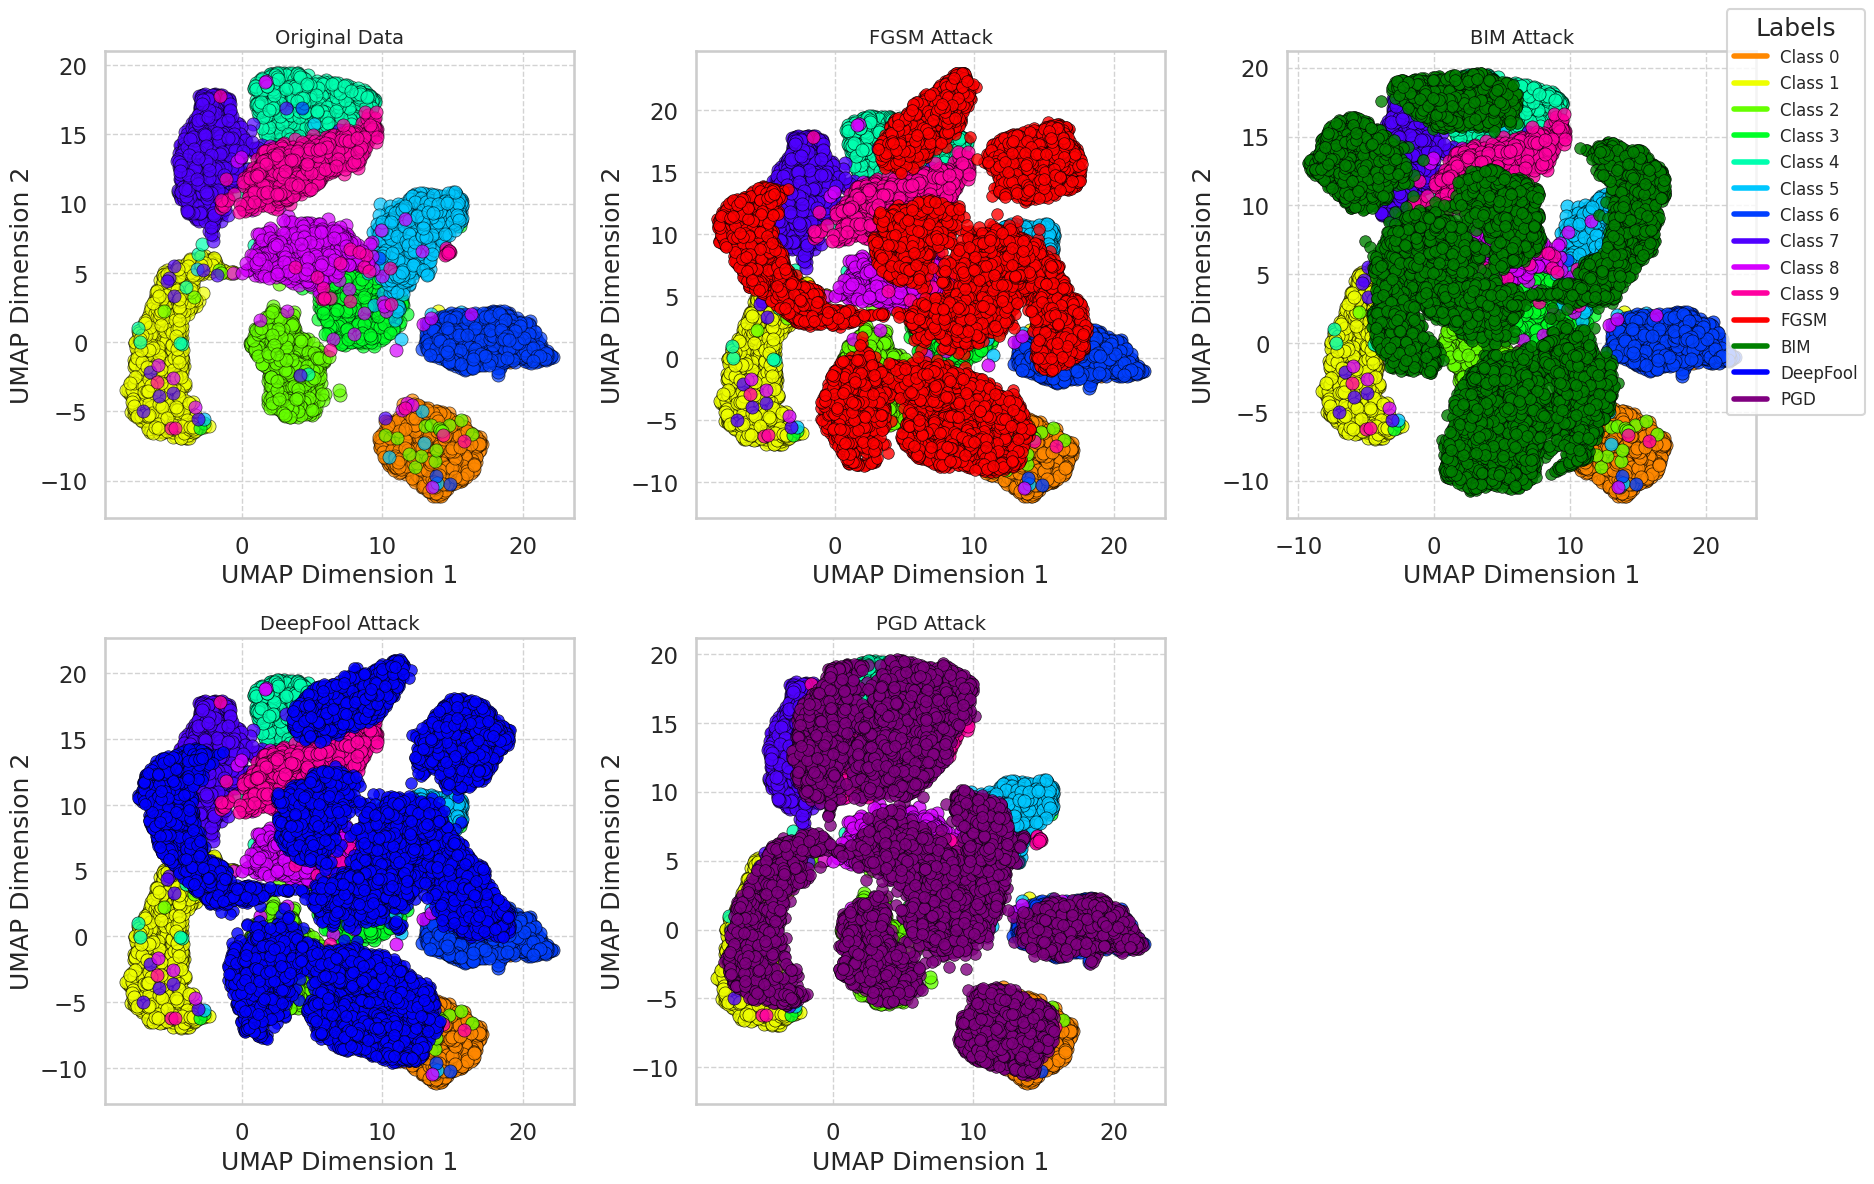
\includegraphics[width=\linewidth]{UMAP/Adversarial Examples.png}
    \caption{Overview of the Proposed Model}
    \label{overview}
\end{figure*}
   
\section{Introduction}

As technology rapidly advances and becomes more integral to our daily lives, the emphasis on the strength and reliability of deep learning models has never been more crucial.These models are increasingly being used in critical safety and socially significant applications like autonomous driving, face recognition, and malware detection, where their efficiency and dependability are of utmost importance. Yet, a key vulnerability lies in deep neural networks' susceptibility to adversarial attacks and natural image perturbations, which can notably degrade their performance. By exploring and improving the robustness of these models, we can ensure their effectiveness and reliability in real-world scenarios \cite {Numair, Aleksandar}.

Adversarial attacks pose significant challenges to these models, exploiting subtle yet critical vulnerabilities. They exploit subtle weaknesses, causing misclassification of examples with imperceptible changes. Such attacks can have a severe impact on the reliability and safety of deep learning models, especially in safety-critical applications like autonomous driving. Adversarial examples can lead to incorrect decisions, potentially resulting in severe consequences. Therefore, it is crucial to analyze the robustness and reliability of deep learning models to ensure their safety in real-world deployments \cite {Samuel, Muhammad}.  To mitigate these challenges, Explainable Artificial Intelligence (XAI) emerges as a pivotal solution, enhancing model transparency and decision-making processes. It helps to enhance the understanding and trustworthiness of AI by providing interpretable and human-understandable explanations of AI decisions. The techniques, tools, and algorithms used in XAI generate explanations that help build trustworthy and interpretable deep learning models. These explanations improve trust by providing insights into the model's decision-making process, addressing challenges of trust, transparency, bias understanding, and fairness, and promoting a more robust and impartial decision-making process \cite {Mohammed, Aha, Tamer}. 

In this study, we venture into a novel exploration of XAI. Existing research predominantly employs SHAP values for adversarial detection  \cite{Fidel, LinY, Stiff, E.Mosca, Tcydenova}, but typically neglects the distinct impacts of positive versus negative SHAP values on model decisions. My work aims to fill this gap by specifically investigating how positive and negative SHAP values differently influence model behavior. This approach is not about outperforming existing detection methods, but about gaining a deeper understanding of model vulnerabilities through a detailed analysis of SHAP value impacts.Our approach uniquely evaluates deep learning model robustness against adversarial attacks, diverging from traditional methods that primarily focus on SHAP values as defensive mechanisms. Contrasting with existing methods that primarily use SHAP values for defensive mechanisms, our research employs pixel-level analysis to understand the impact of influential pixels on model robustness. This approach provides a more granular understanding of how specific pixel manipulations affect the model's performance, offering a novel perspective in evaluating the robustness of deep learning.

% We conducted a research to explore the challenges posed by adversarial attacks on deep learning models. Our primary focus was on understanding and quantifying the impacts of different pixels. To achieve this, we used SHAP (SHapley Additive exPlanations) within the realm of Explainable Artificial Intelligence (XAI) to unravel the complex dynamics of how deep learning models respond to adversarial manipulations. Our goal was not only to identify vulnerabilities but also to enhance the robustness and transparency of these models. The stakes are high in critical applications such as healthcare and autonomous systems. Therefore, our research strives to fortify these models against adversarial threats while simultaneously improving their interpretability and trustworthiness. Through this work, we aim to bridge the existing gap between robustness and transparency in AI, offering novel insights and methodologies that could significantly advance the field.

\section{Contributions of the Paper}

This paper introduces several significant contributions to the field of AI, particularly in enhancing the robustness and transparency of deep learning models against adversarial threats:


\begin{itemize}
    \item \textbf{SHAP Gradient Explainer-based Pixel Analysis:} Pioneering Deep explainer-based pixel-level analysis for adversarial understanding.
    
    \item \textbf{Comprehensive Model Evaluation:} Assessing model robustness across various adversarial perturbations and UMAP visualization is used to improve the interpretability of adversarial impact.
    
    \item \textbf{SHAP Value Comparison:} Analyze critical pixels on different thresholds to reveal subtle adversarial influences.
    
    \item \textbf{Statistical Validation:} Perform statistical validation to strengthen findings in adversarial robustness research.

\end{itemize}

\section{Background and Related Work}

\subsection{Model Architecture and Output Formulation of Deep Neural Networks}



The following is an explanation of a deep neural network classification model denoted by \( F(\cdot) : \mathbb{R}^d \rightarrow [0, 1]^{C} \). Its purpose is to take an image with dimensions \( d = h \times w \times c \) and classify it into one of several categories (output labels) with a probability vector \( F(x) \) of dimensions \( C \). The input to the model is an image vector, and the output is a probability distribution of all possible labels, where \( F(x)_i \)  is the probability that the input vector \( x \)  is labeled with \( i \). 

The Logits of the final layer of a Deep Neural Network (DNN) is represented by \(L(\cdot)\), and the model output is calculated by using the softmax activation function on Logits. This can be expressed as \cite {ZhangS.}:

\begin{equation}
    F(x) = \text{softmax}(L(x)).
    \end{equation}

The label with the highest probability in \( F(x) \) is the predicted label of an input image \( x \), and it looks like this \cite {ZhangS.}: 
\begin{equation}
    \hat{y} = \arg\max_i (F(x)_i).
    \end{equation}

Let's assume that the deep neural network has \( l + 1 \) layers, with the input layer being the 0-th layer and the output layer being the \( l \)-th layer. The output of the \( i \)-th neural network layer is denoted as \( F_i(\cdot) \).

\subsection{Adversarial Attacks and Defense Mechanisms} 

The process used to create adversarial samples is called an adversarial attack model. It involves using a model, denoted by  \( F(\cdot) \), and an original input image, denoted by \( x \), to create an adversarial sample, denoted by \( x' = x + d \) , by introducing a specific perturbation to \( x \). This perturbation, denoted by \( d \), causes the model to predict a different label for the adversarial sample \( x' \) than it would for the original sample \( x \) \cite {ZhangS.}.

\begin{align}
    \hat{y}' &\neq \hat{y}, \\
    \text{where } \hat{y} &= \arg\max_i (F(x)_i) \text{and} \\
    \hat{y}'&= \arg\max_i (F(x')_i),
\end{align}

The perturbation \( \|d\| < \epsilon \) must have an absolute value less than epsilon, where epsilon represents the maximum perturbation size. 
According to the research \cite {Ilyas.}, the existence of adversarial examples in a dataset is an intrinsic property. The authors introduce the concept of robust and non-robust characteristics to classify dataset features. Non-robust features exhibit high predictive power but also exhibit highly vulnerable to significant changes when slight perturbations are introduced to the input. Conversely, robust features possess high predictive power and are resistant to slight changes in the input. Robust features are considered as fundamental aspects of the target class, such as the presence of wheels and windows in cars. Non-robust features are seemingly arbitrary patterns that are not easily noticable by humans but demonstrate strong predictive power during the training phase. The work of \cite {Ilyas.} illustrates that non-robust features play a significant role in the generation of adversarial examples and their ability to move between different classification models. These non-robust features are vulnerable to minor perturbations in the input, which can result in significant changes in the value of these highly predictive features.

Several techniques for generating adversarial examples have been developed in recent years. Some of the most prominent options that we utilize for our assessment include:


\subsubsection{Fast Gradient Sign Method (FGSM) \cite {Goodfellow.}}

Adversarial samples are generated by the Fast Gradient Sign Method (FGSM), which utilizes the linear properties of deep neural networks. In this method, the adversarial example \( x' \) is obtained by :
\begin{equation}
    x' = x + \epsilon \cdot \text{sign}(\nabla_x J(x, y));
\end{equation}

Here, \( x \) represents the original image, \( x' \) represents the adversarial example, \( J \) refers to the loss function, and \( \epsilon \) is the perturbation limit. This technique modifies the pixels uniformly based on the gradient of the loss function.



\subsubsection{Basic Iterative Method (BIM) \cite {Kurakin., Madry.}}

The Basic Iterative Method (BIM), proposed by Alexey and colleagues, is an extension of the FGSM method that progressively improves upon it. In each step, a minor disturbance is introduced by the following equation: 
\begin{equation}
    x'_{i} = \text{clip}_{x, \epsilon} \left( x'_{i-1} + \epsilon \cdot \text{sign}(\nabla_{x'_{i-1}} L(x'_{i-1}, y)) \right);
    \end{equation}
The BIM algorithm starts with an initial value of \( x'_0 = x \), and a clipping function is applied to ensure that the modified image remains within specified boundaries. The iterative nature of this method enables more precise fine-tuning compared to the FGSM method.


\subsubsection{Projected Gradient Descent (PGD) \cite {Stiff}}

PGD, an extension of FGSM, adopts a multi-step approach:
\begin{equation}
x'_0 = x \quad 
\end{equation}
\begin{equation}
x'_{t+1} = \text{clip}_{[0,1]} \left( x'_t + \alpha \cdot \text{sign}(\nabla J_\theta(x'_t, l)) \right)
\end{equation}
The \(\text{clip}_{[0,1]}(\cdot)\) function ensures the perturbed image remains within [0, 1]. PGD is computationally intensive but offers a stronger and more precise attack than FGSM.



Projected Gradient Descent (PGD) is a technique that is derived from the Fast Gradient Sign Method (FGSM).
\begin{equation}
    x'_0 = x \quad 
    \end{equation}
    \begin{equation}
    x'_{t+1} = \text{clip}_{[0,1]} \left( x'_t + \alpha \cdot \text{sign}(\nabla J(\theta, x'_t, l)) \right)
    \end{equation}

The perturbed image is then clipped to the range of [0,1] using the function \(\text{clip}_{[0,1]}(\cdot)\). This process is performed until a certain number of iterations is reached. The PGD algorithm requires a significant amount of computational resources, but it provides a more robust and accurate method of attack compared to the FGSM.


\subsubsection{DeepFool}

DeepFool \cite {Moosavi} is an algorithm that aims to generate adversarial examples with minimal perturbation. The algorithm minimizes the \(L_2\) norm and iteratively applies small perturbations to an input image using a linear neural network. The objective of DeepFool is to find the smallest perturbation required to change the classification of an input image. The algorithm computes the perturbation by solving the following optimization problem:

\begin{equation}
r^*(x_0) = \arg\min_r \|r\| \quad \text{s.t.}
\end{equation}
\begin{equation} 
\quad \text{sign}(f(x_0 + r)) \neq \text{sign}(f(x_0)),
\end{equation}

The solution to this problem can be approximated using the gradient of the neural network. When the gradient is not available, DeepFool uses an approximation based on the linearization of the neural network. The perturbation is computed as follows:

\begin{equation}
r^*(x_0) = \frac{|f(x_0)|}{\|w\|^2} w.
\end{equation}

DeepFool can also be used to generate targeted adversarial examples. In this case, the algorithm solves the following optimization problem:

\begin{equation}
\arg\min_{r_i} \|r_i\|^2 \quad \text{s.t.} 
\end{equation}
\begin{equation}
\quad f(x_i) + \nabla f(x_i)^T r_i = 0.
\end{equation}

DeepFool has been shown to be effective in generating adversarial examples with comparable accuracy to FGSM but with less perturbation.



Some examples of defense methods against adversarial example include adversarial training \cite {Goodfellow.}, Defensive Distillation \cite {Papernot}, Gradient Obfuscation, Feature Squeezing \cite {Evans}, ML-LOO \cite {Yang}, Density Estimates \cite {Feinman}, Local Intrinsic Dimensionality \cite {Ma}, Mahalanobis Distance 
 \cite {Lee}, SHAP signatures \cite{Fidel, LinY, Stiff, E.Mosca, Tcydenova} and many more. In our research, we propose a method for identifying critical pixels in both normal and adversarial examples. This will aid in the generation and defense of attacks. 


\subsection{Explainable AI}

Explainable AI (XAI) plays a crucial role in the field of deep learning as it enables AI systems to be transparent and comprehensible. Its main objective is to establish confidence and effectively handle complex AI solutions. The role of XAI is particularly important in supervised models as it enables a comprehensive explanation of the reasoning behind predictions. Prominent XAI technique is SHAP, used for additive feature attribution. It involves explaining Shapley values, which are a way to assign credit to input features for the output of a model. SHAP combines the Shapley value method with the local interpretable model-agnostic explanations (LIME) \cite {Ribeiro} technique. Many explanation methods for deep learning models use additive feature attribution methods, such as LIME, DeepLIFT \cite {Shrikumar}, layer-wise relevance propagation, Shapley regression values, Shapley sampling values and quantitative Input Influence. There are several explainers in SHAP \cite {LundbergandS}, including the tree explainer, gradient explainer, kernel explainer, deep explainer and sampling explainer. The tree explainer is a fast and exact method for estimating SHAP values for tree models and ensembles of trees. The gradient explainer can explain a model using expected gradients. The kernel explainer uses a particular weighted linear regression to compute the importance of each feature. The deep explainer is an enhanced version of the DeepLIFT algorithm that approximates the conditional expectations of SHAP values using a selection of background samples. The sampling explainer is an extension of the Shapley sampling values explanation method \cite{ZhangK}. Our work centers around a thorough pixel-level examination using the Deep Explainer method, providing a unique perspective on adversarial understanding.


% It is widely used in various domains such as engineering \cite{Mangalathu}, aerospace \cite{Aouf}, medical \cite{Singh},  transportation \cite{Parsa}, manufacturing \cite{Huang}, security \cite{Warnecke}, and others due to its ability to analyze complex models. 

% DeepSHAP has proven to be crucial in detecting adversarial examples. It is used in image detection to differentiate between adversarial and normal samples, as well as for identifying word-level adversarial attacks.

Our study expands the applicability of SHAP values beyond being just a general XAI indicator. Instead, we use SHAP values to specifically pinpoint crucial pixels, thus increasing our understanding of adversarial attack manipulations and strengthening the resilience of AI models.


\section{Proposed Methodology:}

\begin{figure*}[!ht]
    \centering
    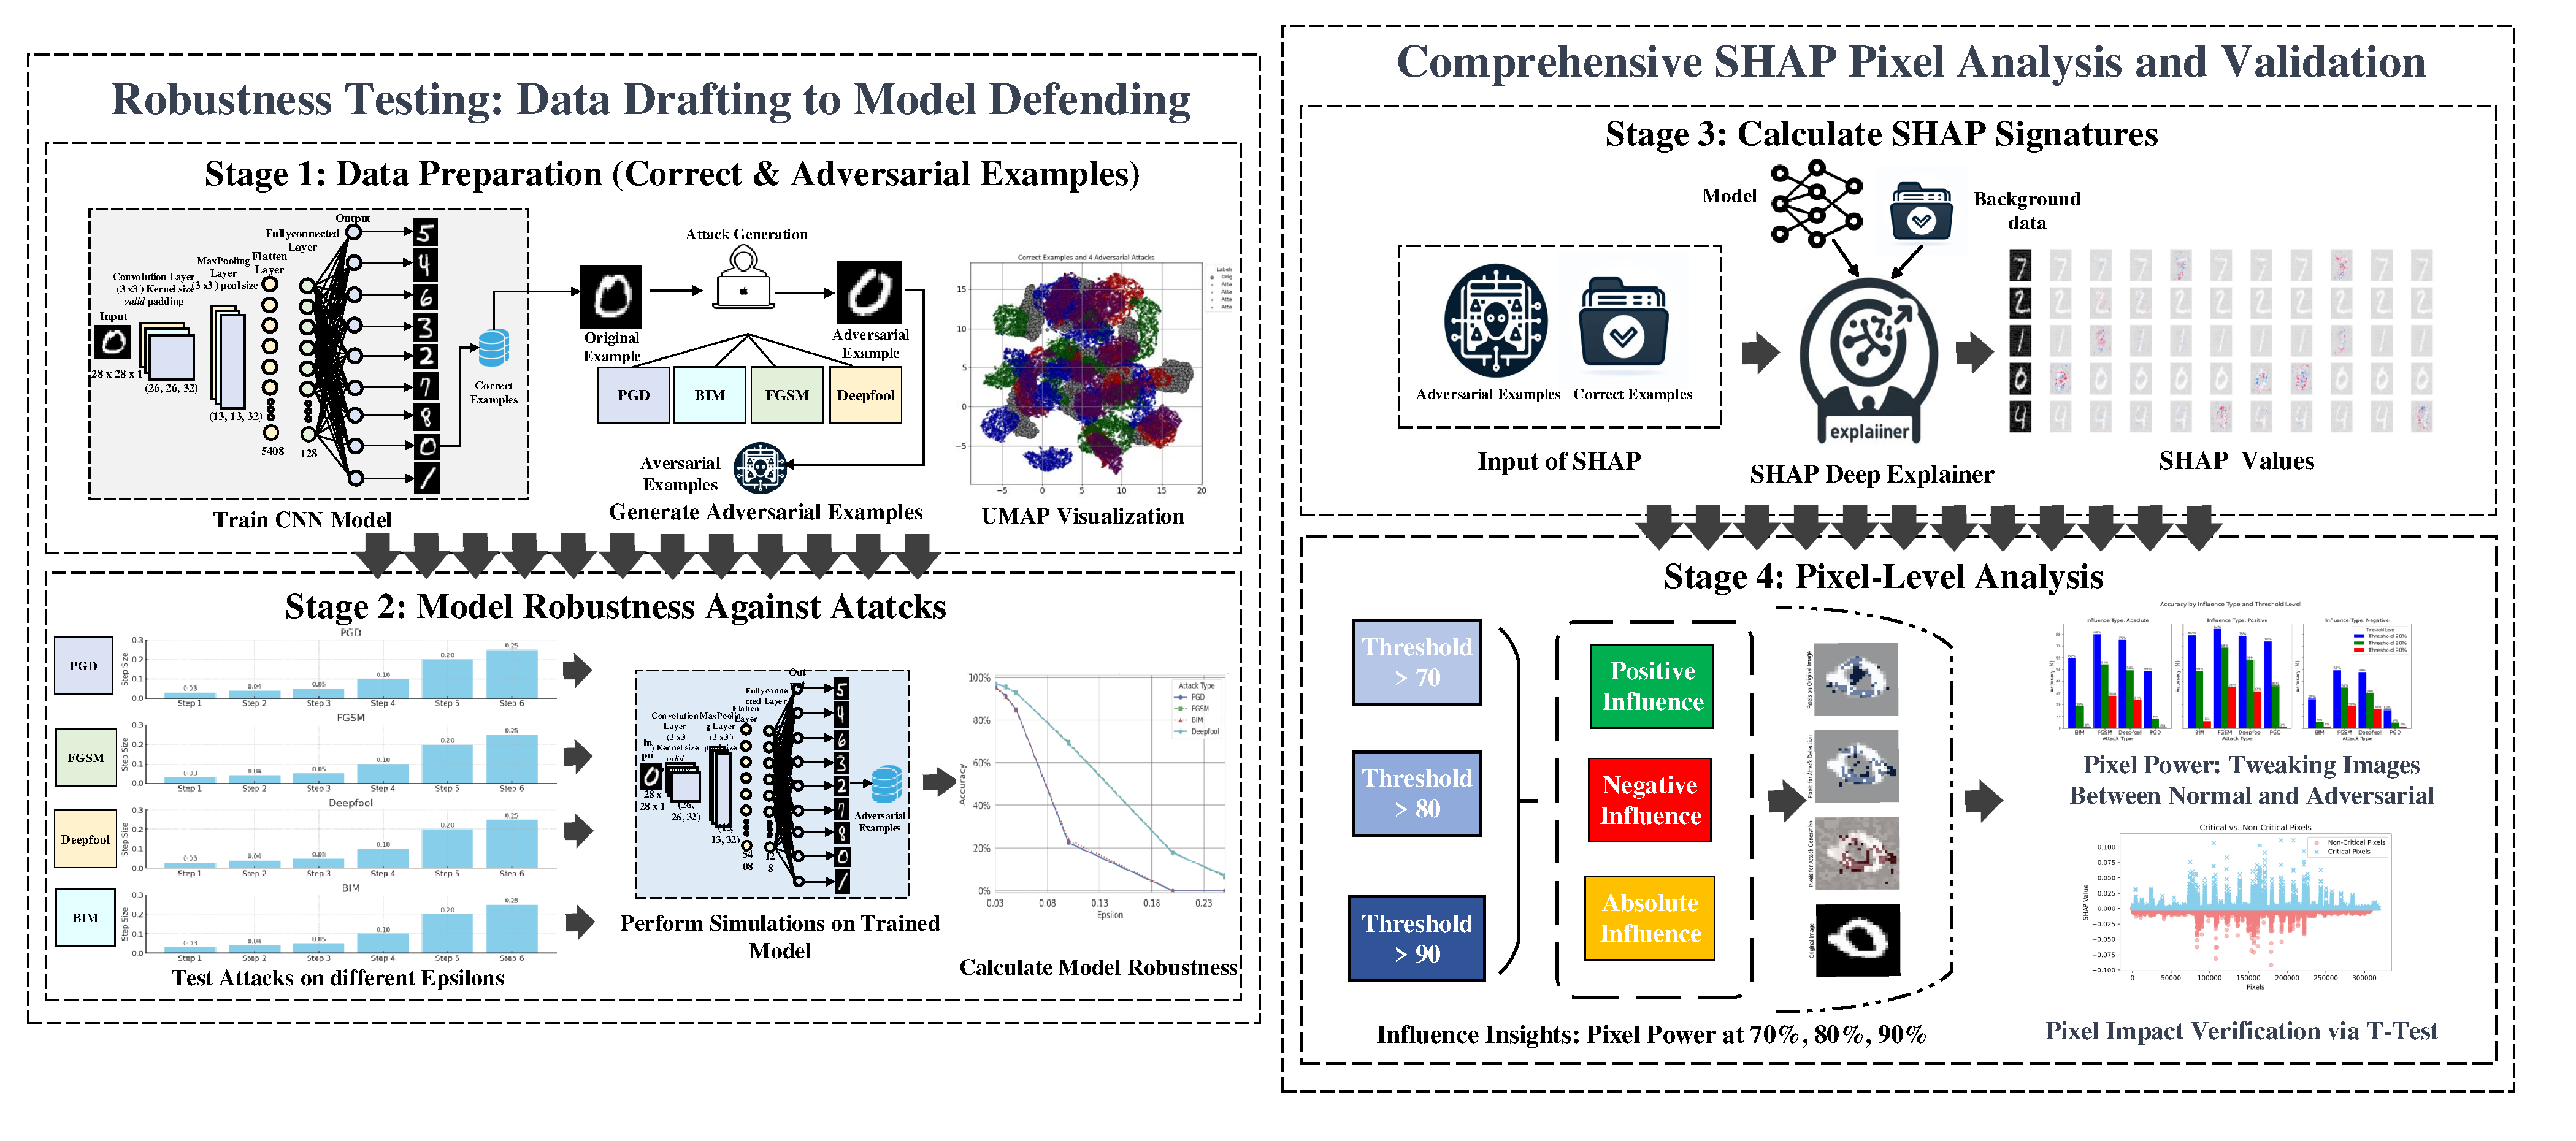
\includegraphics[width=\linewidth]{Model/EuroML_V2.pdf}
    \caption{Overview of the Proposed Model}
    \label{overview}
\end{figure*}
   
Our research, depicted in Figure. \ref{overview}, focuses on robustness testing and a comprehensive SHAP pixel analysis. We employed a CNN model and the MNIST dataset for training, with a primary focus on achieving accurate image identification. Afterward, we exposed our model to complex simulated attacks to gauge its robustness. Subsequently, we carried out an extensive analysis of the influence of various step sizes on its decision-making mechanism.

In the final phase, we identify critical pixels in both normal and adversarial examples, examining their influence on model accuracy, whether positive or negative. This aspect, often overlooked in the literature, forms a key part of our study. To validate our findings, we employ the t-test. Our model rigorously explores the effects of various perturbation sizes in adversarial attacks on deep learning models and analyzes pixel shifts in both adversarial and normal images.


\subsection{Stage 1: Data and Model Preparation}

In the initial phase, we utilized a CNN model to train on the MNIST dataset for digit classification. To ensure a well-rounded investigation, creating a dataset comprising only correctly predicted examples. The correctly classified examples consisted of 973 instances labeled as 0, 1133 as 1, 1016 as 2, 989 as 3, 969 as 4, 882 as 5, 937 as 6, 1005 as 7, 946 as 8, and 984 as 9. Next, we employed the Foolbox Python library to execute various adversarial attacks, including BIM, FGSM, DeepFool, and PGD. While generating adversarial examples it is crucial to investigat attack paprameter such as distance metric. The distance metric is used to measure the perturbation, which can be quantified by three norms: \( l_0 \), \( l_2 \), and 
\( l_{\infty} \). The \( l_0 \) norm counts the number of altered non-zero elements, or the number of pixels that have been modified by the adversarial attack in the original image. The \( l_2 \) norm refers to the conventional Euclidean distance, which is obtained by summing the squares of the modified elements and then taking the square root. The \( l_{\infty} \) norm represents the highest value among all the elements of the perturbation. By default, in this paper we uses the 
\( l_{\infty} \) norm to quantify the magnitude of the disturbance. Figure. \ref{fig:umap}(a) provides a UMAP visualization of the MNIST dataset, with each point representing a digit from 0 to 9. Original digit classes are color-coded, while the PGD attack-generated adversarial examples are intermixed within these clusters, as depicted in \ref{fig:umap}(b). This visual representation aids in understanding how adversarial perturbations impact classification accuracy and identifying model vulnerabilities. By deriving insights from this analysis, we aim to enhance the model's robustness and ensure its reliability against adversarial threats in real-world scenarios.

\begin{figure*}[!ht]
    \centering
    \begin{subfigure}{.25\textwidth}
        \centering
        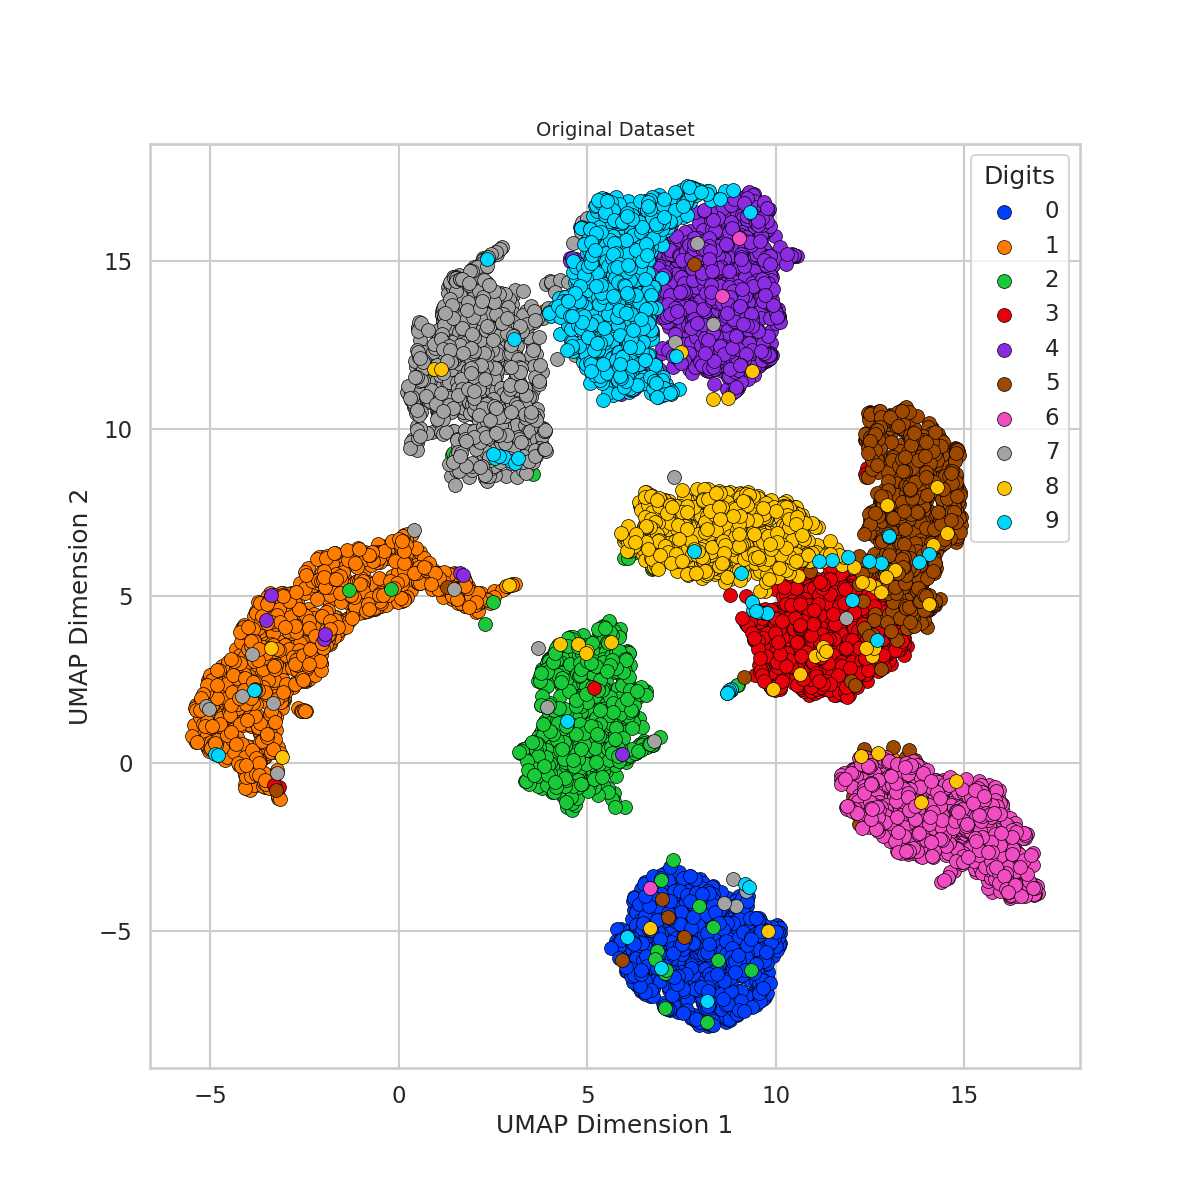
\includegraphics[width=\linewidth]{UMAP/UMAP_Original Dataset.png}
        \caption{Original MNIST digit classes}
        \label{fig:umap_original}
    \end{subfigure}%
    \hfill
    \begin{subfigure}{.25\textwidth}
        \centering
        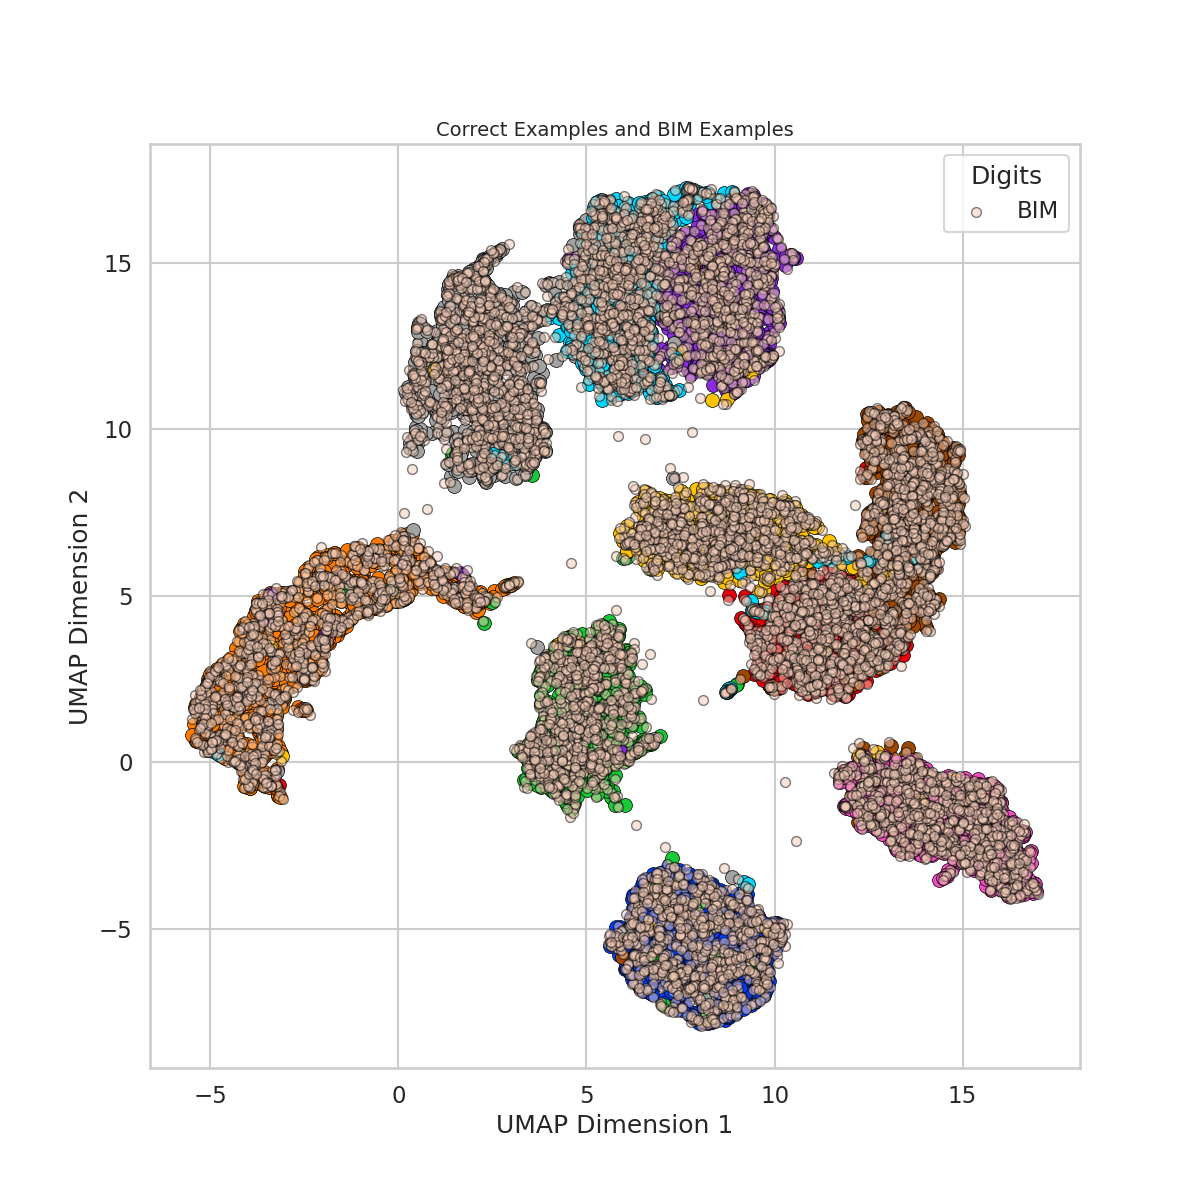
\includegraphics[width=\linewidth]{UMAP/UMAP_Combined_BIM.png}
        \caption{Original and PGD attack}
        \label{fig:umap_pgd}
    \end{subfigure}
    \hfill
    \begin{subfigure}{.25\textwidth}
        \centering
        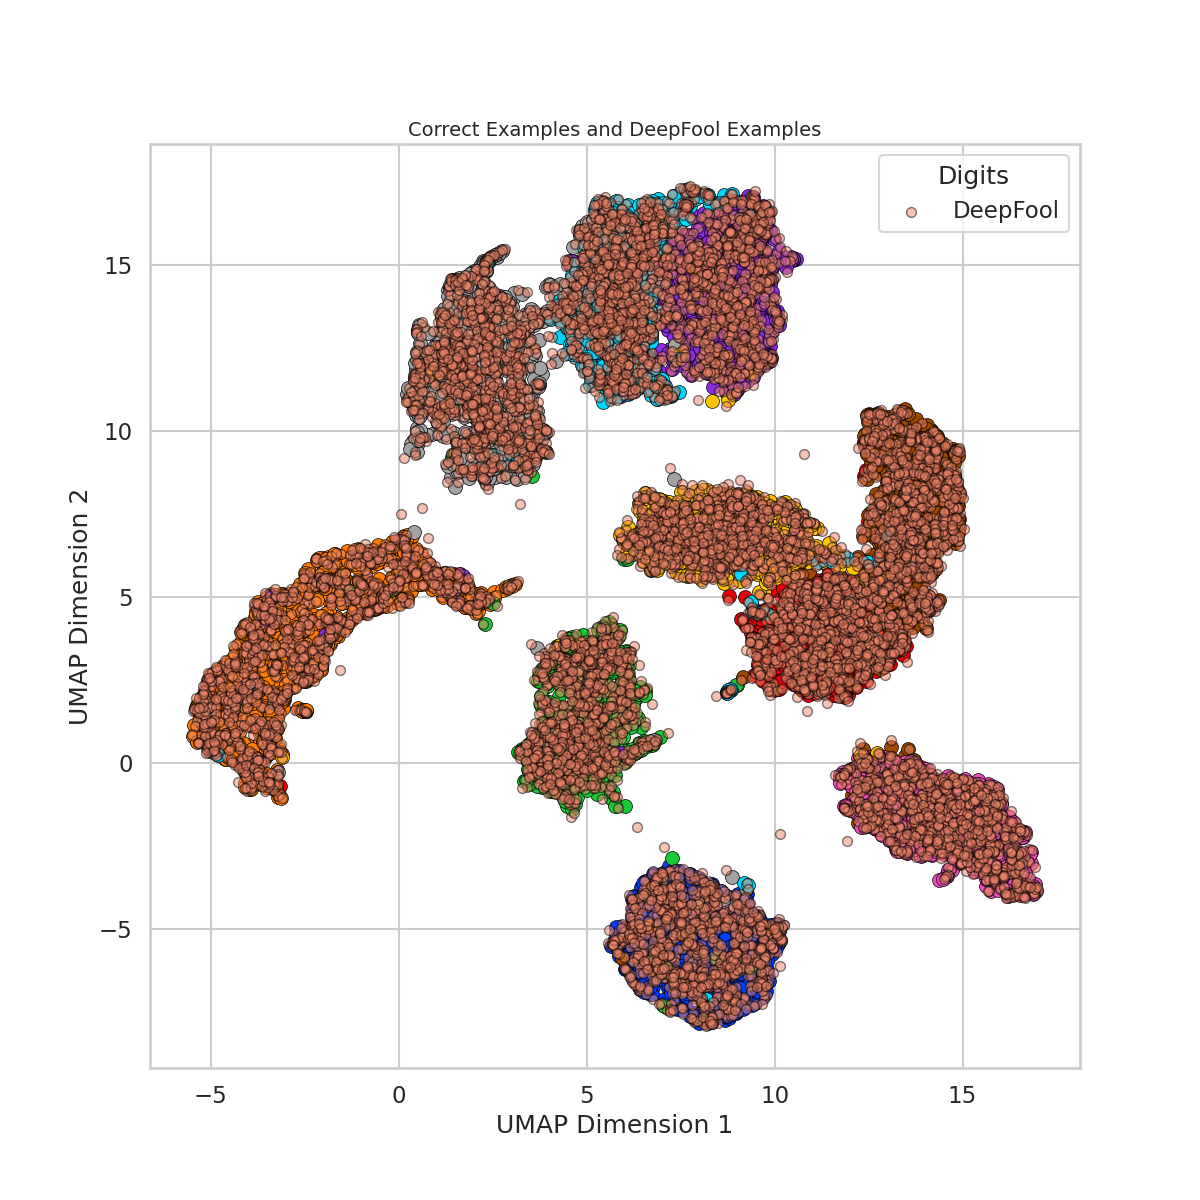
\includegraphics[width=\linewidth]{UMAP/UMAP_Combined_DeepFool.png}
        \caption{Original and PGD attack}
        \label{fig:umap_pgd}
    \end{subfigure}
    \hfill
    \begin{subfigure}{.25\textwidth}
        \centering
        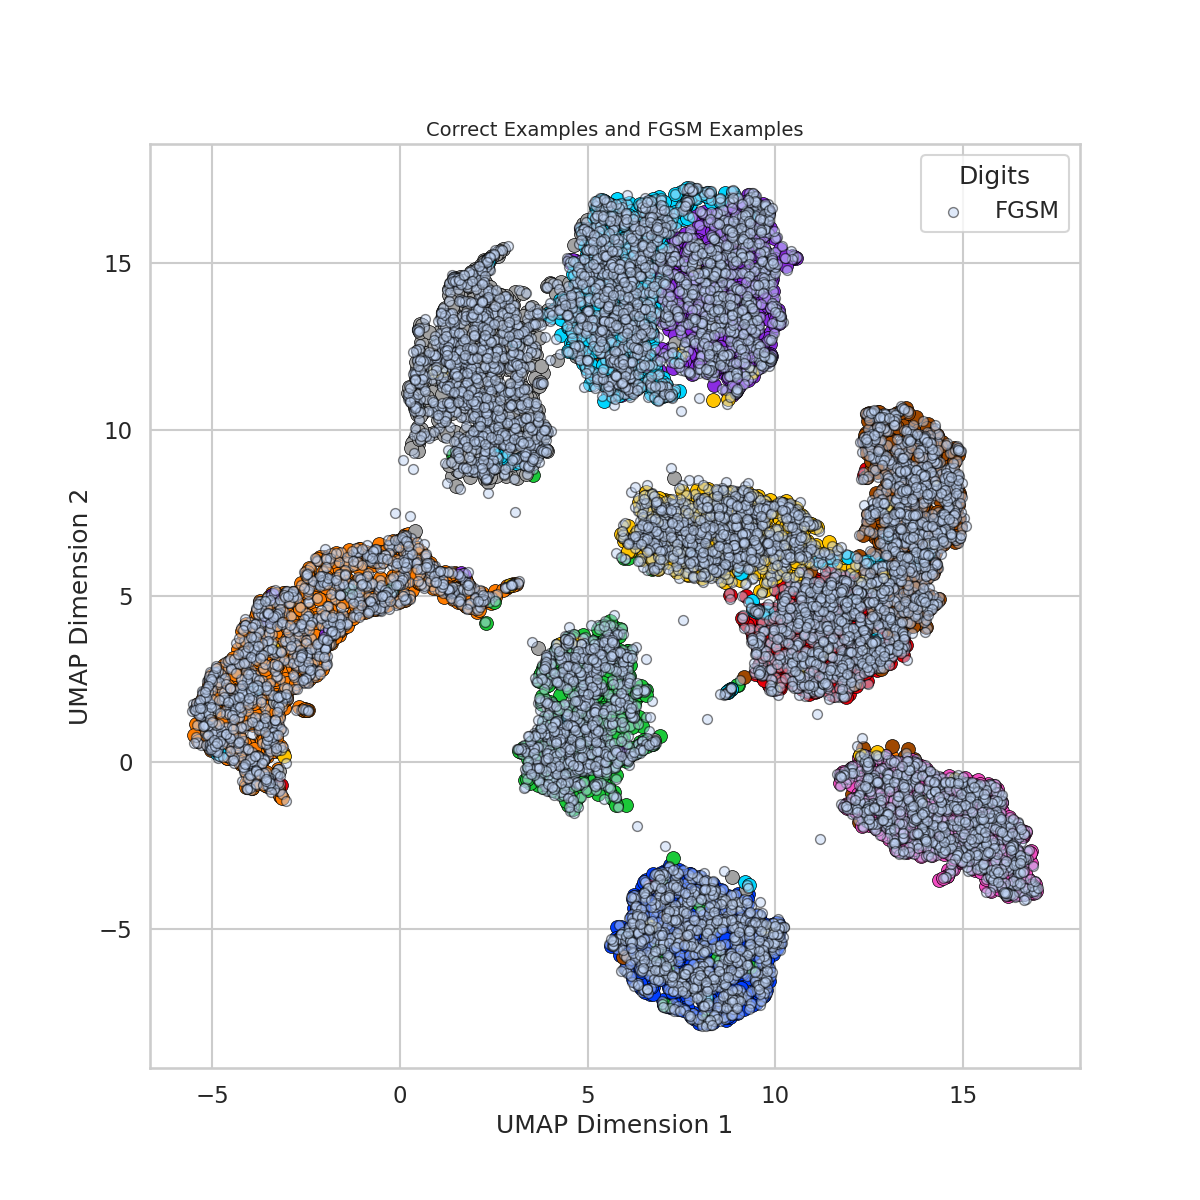
\includegraphics[width=\linewidth]{UMAP/UMAP_Combined_FGSM.png}
        \caption{Original and PGD attack}
        \label{fig:umap_pgd}
    \end{subfigure}
    \hfill
    \begin{subfigure}{.25\textwidth}
        \centering
        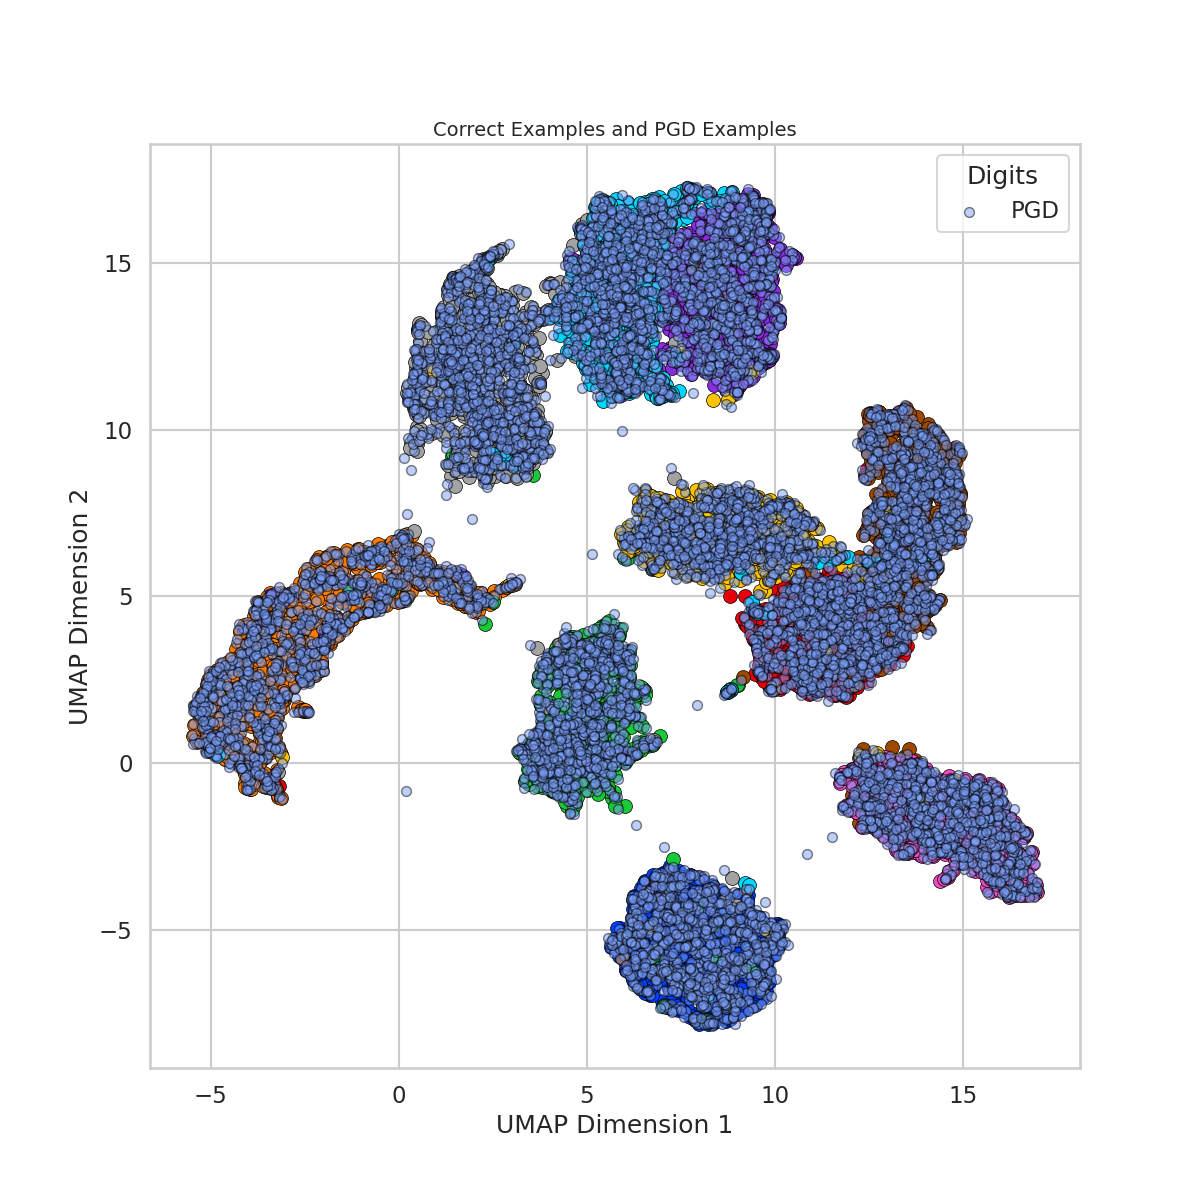
\includegraphics[width=\linewidth]{UMAP/UMAP_Combined_PGD.png}
        \caption{Original and PGD attack}
        \label{fig:umap_pgd}
    \end{subfigure}
    \caption{UMAP projections illustrating the separation of digit classes within the MNIST dataset and the integration of adversarial examples.
     The left panel (\ref{fig:umap_original}) shows the natural clustering of MNIST digits, and the right panel panel (\ref{fig:umap_pgd}) overlays PGD 
     adversarial examples.}
    \label{fig:umap}
\end{figure*}

\subsection{Stage 2: Model robustness against Attacks}
We systematically collected and analyzed the resulting adversarial examples, subsequently subjecting them to model testing to evaluate its robustness under deliberately misleading conditions. To create varying levels of perturbation, we selected a range of epsilon values set at [0.03, 0.04, 0.05, 0.1, 0.2, 0.25]. This approach allowed us to comprehensively investigate how the model responded to different levels of adversarial intensity, a critical factor in assessing its overall robustness.


\subsection{Stage 3: Extraction of XAI Signatures}

In this stage of our research, we employed the Deep Explainer, a specialized component within the SHAP (SHapley Additive exPlanations) framework, tailored for deep learning models. Deep Explainer operates by approximating SHAP values, which quantify the contribution of each input feature, or in this case, each pixel, to the model's prediction for a given instance. Deep Explainer works by using a reference set of 'background' data points to approximate how the absence or presence of features in the input data influences the model’s output. In our study, it systematically analyzed the input pixels of an image, comparing how each pixel's presence or alteration (especially in adversarial cases) affects the model's output. By aggregating these effects, Deep Explainer provided a detailed map of pixel-level contributions to the final prediction. By calculating these SHAP values for specific subsets of our data, this approach helped us identify significant differences in their influence on the model's predictions. It allowed us to gain valuable insights into the model's decision-making process when presented with adversarial examples.

In this stage of our research, we outlined our approach for investigating the influence of individual input pixels on the model's predictive behavior under normal and adversarial conditions. Central to our methodology was the application of the SHapley Additive exPlanations (SHAP) framework, with a specific focus on the Deep Explainer module, designed to elucidate the contributions of individual features in deep learning models.

The process commenced with the selection of background data for the SHAP analysis. We chose a subset of 3000 instances of correctly and adversairial classified examples within our dataset. To rigorously assess the model's behavior under adversarial attacks, we incorporated a range of attack methodologies including Basic Iterative Method (BIM), Fast Gradient Sign Method (FGSM), DeepFool, and Projected Gradient Descent (PGD). For each attack type, we established a systematic approach to calculate and store SHAP values. This involved creating a multidimensional structure indexed by attack type and epsilon value, the latter of which was predetermined to reflect various intensities of adversarial perturbation. Within this framework, for each attack type and epsilon level, we curated a batch of up to 200  adversarial examples. These examples were then preprocessed to conform to the input requirements of the SHAP Deep Explainer. It involved converting the examples into a format amenable to analysis, such as NumPy arrays, ensuring compatibility with the underlying computational framework of SHAP. Employing the Deep Explainer, we computed SHAP values for these examples, facilitating a detailed and granular analysis of pixel-level contributions to the model’s output. This computation was instrumental in discerning the influence of individual pixels on the model's decision-making process, especially when subjected to varying adversarial conditions.



% \begin{figure}[h]
% \centering
% \begin{subfigure}{\columnwidth}
% \centering
% 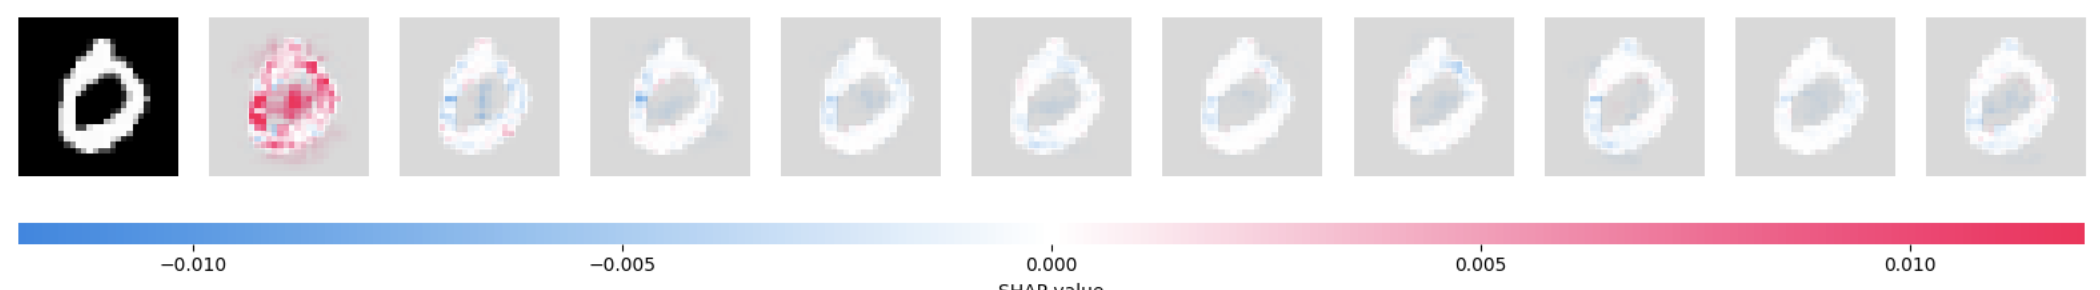
\includegraphics[width=\linewidth]{paper_images/normal.png}
% \label{fig:correct_shap}
% \end{subfigure}
% \par\medskip
% \begin{subfigure}{\columnwidth}
% \centering
% 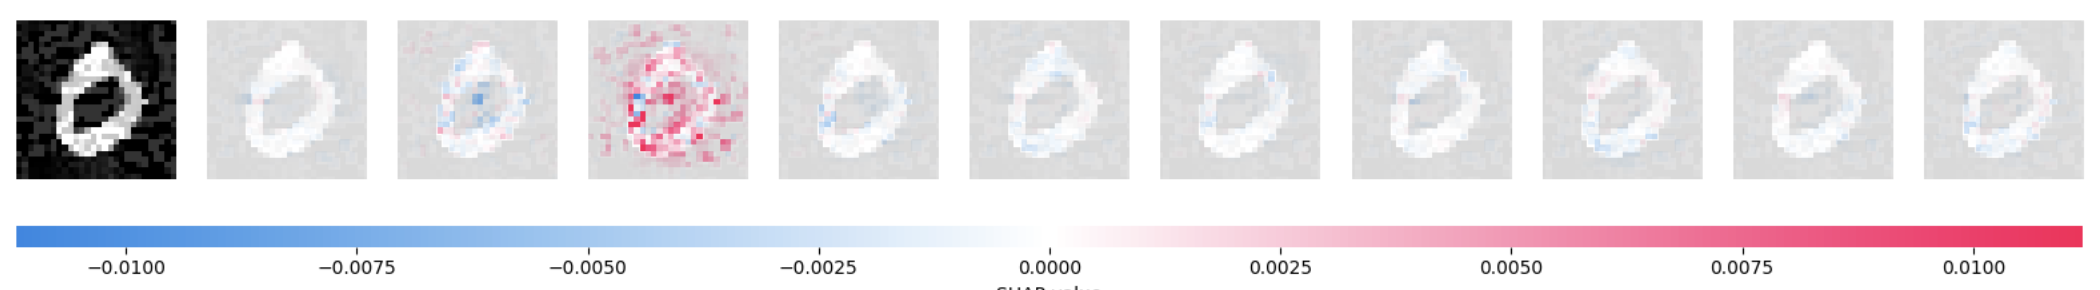
\includegraphics[width=\linewidth]{paper_images/pgd.png}
% \label{fig:pgd}
% \end{subfigure}
% \begin{subfigure}{\columnwidth}
% \centering
% 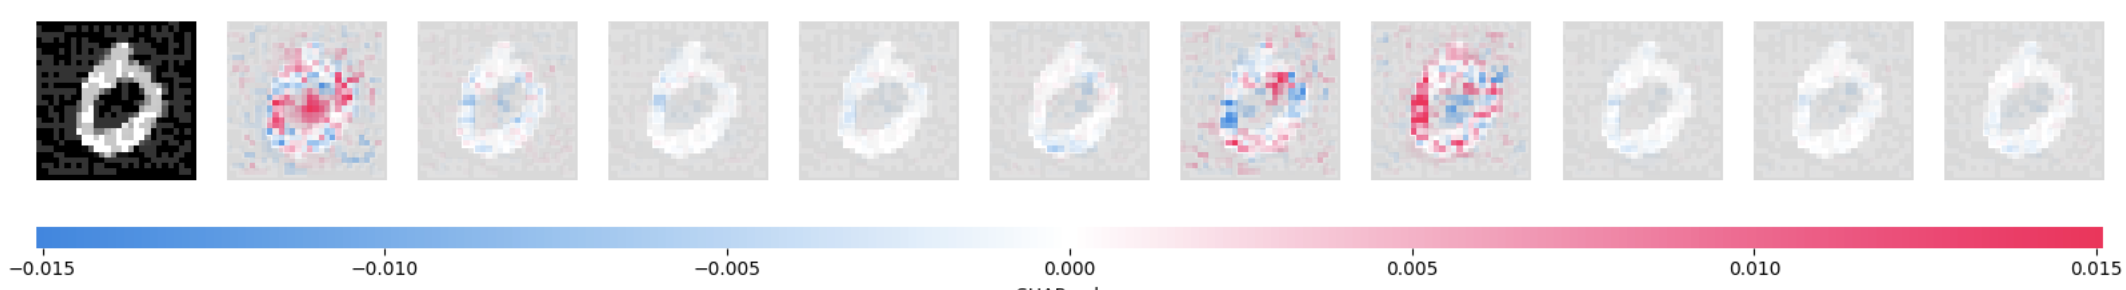
\includegraphics[width=\linewidth]{paper_images/fgsm.png}
% \label{fig:fgsm}
% \end{subfigure}
% \begin{subfigure}{\columnwidth}
% \centering
% 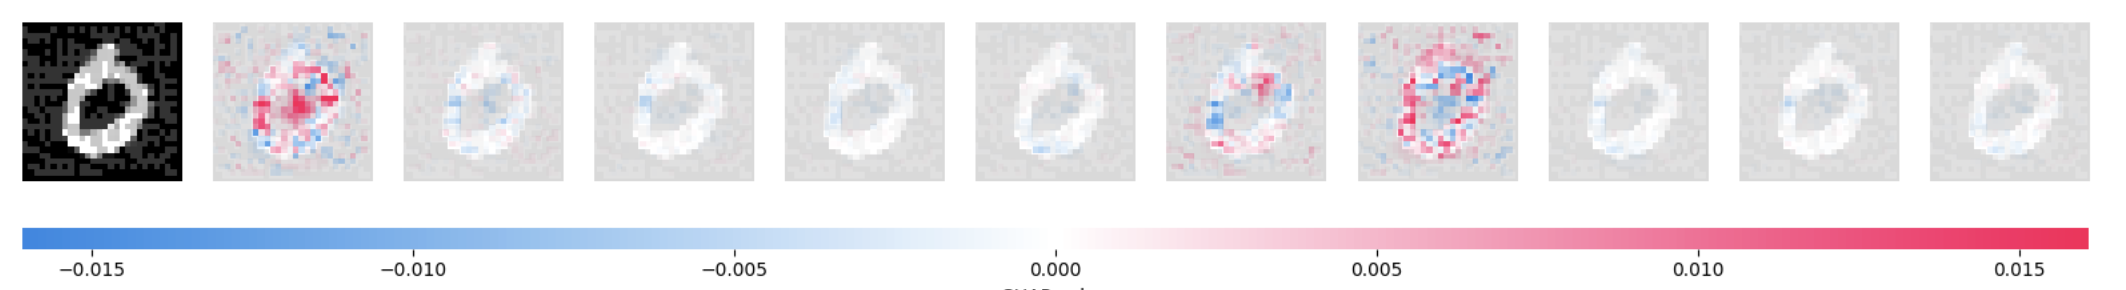
\includegraphics[width=\linewidth]{paper_images/deep.png}
% \label{fig:deep}
% \end{subfigure}
% \begin{subfigure}{\columnwidth}
% \centering
% 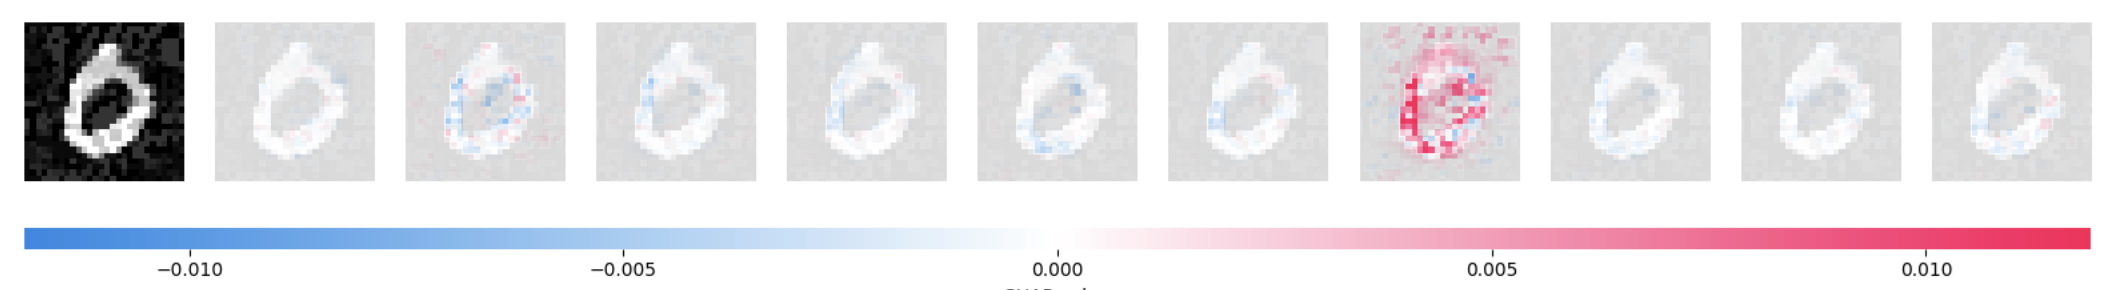
\includegraphics[width=\linewidth]{paper_images/basic.png}
% \label{fig:basic}
% \end{subfigure}
% \caption{SHAP heatmaps depicts the interpretability of a model's decision for a normally classified digit and its progressive alteration under various adversarial attacks (PGD, FGSM, deepfool and basic iterative method), highlighting the shift in influential pixels at a granular level. (a): Normal, (b): PGD, (c): FGSM, (d): Deep Fool, (e): BIM}
% \label{fig:both_shap_figures}
% \end{figure}



    
\section{Stage 4: Pixels Level}

We have implemented approach to modify both normal and adversarial images using SHAP values. This process is essential for understanding how different pixels influence a deep learning model predictions, especially under adversarial conditions. Let me detail this process:

\subsection{Modification of Normal Images:}

 For each normal image, SHAP values are computed to determine the influence of each pixel on the model's prediction. A threshold is applied to these SHAP values to identify pixels with the most significant influence. This threshold is varied (70\%, 80\%, and 90\%) to assess different levels of influence. Influential pixels (those exceeding the threshold in their absolute, positve and negative SHAP value) are modified. This modification typically involves reducing the pixel intensity, which allows for an investigation into how such alterations affect the model's prediction accuracy.

\subsection{Modification of Adversarial Images:}
For each adversarial image, its corresponding normal (unperturbed) image is also considered. SHAP values for the adversarial image are calculated. Similar to the normal images, a threshold is applied to the SHAP values. The influence types are 'absolute', 'positive' and 'negative' determine how the threshold is computed and applied. For pixels in the adversarial image that exceed the threshold, they are replaced with their counterparts from the normal image. This step is crucial as it helps in understanding how reverting the most influential pixels to their original state affects the model's performance. After modifying the images (both normal and adversarial), these images are fed into the model to obtain predictions. The model's accuracy is then evaluated by comparing these predictions against the true labels. The accuracy data, along with other parameters like image index, attack type, epsilon value, threshold level, and influence type, are compiled into a DataFrame. This structured data allows for a comprehensive analysis of how the model's accuracy is impacted by the modifications made to both normal and adversarial images.

It provides detailed insights into which pixels significantly affect the model's predictions, under both normal and adversarial conditions. By comparing the model's performance on modified versus original images, you can gauge the model's vulnerability to specific types of pixel-level perturbations. Understanding how pixel modifications affect accuracy can guide efforts to enhance the model's robustness against adversarial attacks.

    
\subsubsection{Statistical Validation of Critical Pixels}


In our validation phase, we employed a one-sample t-test to confirm the statistical significance of pixel influences identified using SHAP values. The t-test assessed whether these influences, especially the positively impactful ones, significantly deviated from a null hypothesis of zero influence. A high t-statistic indicated a substantial deviation, implying meaningful pixel impact. The associated p-value, nearly zero, underscored the statistical significance of these influences. This rigorous statistical validation enhances the credibility of our findings, confirming that the identified pixels have a genuine and statistically substantiated impact on the model's decision-making process, strengthening our research's scientific validity.
    % \begin{table*}[t]
    %     \centering
    %     \begin{tabular}{|p{3cm}|p{6cm}|}
    %     \hline
    %     \textbf{SHAP Value Proximity to Zero} & \textbf{Interpretation} \\ \hline
    %     Close to Zero & 
    %     \begin{itemize}
    %     \item Feature has minimal impact on the model's prediction.
    %     \item Changes in the feature value do not significantly affect the prediction.
    %     \item Feature is considered neutral or weak in terms of prediction influence.
    %     \end{itemize}
    %     \\ \hline
    %     Far from Zero (Positive or Negative) & 
    %     \begin{itemize}
    %     \item Feature has a substantial impact on the model's prediction.
    %     \item Variations in the feature value lead to significant changes in the prediction.
    %     \item Feature is a strong influencer of the predicted outcome.
    %     \item The magnitude of the SHAP value indicates the strength of the feature's influence.
    %     \end{itemize}
    %     \\ \hline
    %     \end{tabular}
    %     \caption{Interpretations of SHAP Values Based on Proximity to Zero}
    %     \label{table:shap-value-interpretation}
    % \end{table*}
    
    

% In Stage 5 of our research, we focused on the development of a binary classification model that could effectively differentiate between original and adversarial examples. The crux of this stage was the utilization of XAI signatures, particularly SHAP values, instead of raw data. The choice of XAI signatures was strategic and stemmed from the need for deeper insights into the decision-making processes of neural networks. These signatures, unlike raw data, provide a nuanced understanding of feature importance and contributions, making them immensely valuable in identifying subtle manipulations in adversarial examples.

% This approach aligns with the broader objective of enhancing the interpretability and trustworthiness of deep learning models. By using XAI signatures, we aim to gain a more transparent view into how and why models make certain decisions, especially under adversarial conditions. This transparency is crucial for identifying potential vulnerabilities and strengthening the model's defenses against sophisticated attacks.

% Moreover, understanding the influence of individual features on model predictions through XAI signatures aids significantly in the research and development of more robust attack detection methods. It enables us to pinpoint which features are most exploited in adversarial attacks and thus devise more effective strategies to counter them.

% For the testing phase, we opted for a simple neural network model. This choice was deliberate; a simpler model allows for clearer interpretation of results and a more straightforward evaluation of the effectiveness of XAI signatures. It serves as a preliminary testing ground, where we can assess the viability of our approach before scaling up to more complex models. This step is essential in ensuring that our methodology is sound and effective in a controlled environment before applying it to more intricate and real-world scenarios.
% Evaluate the classification model's performance in correctly identifying adversarial attacks.

\section{Experiments:}

In our evaluation we aimed to answer the following two research questions:
\begin{itemize}
    \item\textbf{RQ1:} How effective is SHapley Additive exPlanations (SHAP) analysis in identifying specific pixel-level vulnerabilities in deep learning models, and what insights does it provide for understanding the nature of these vulnerabilities?
    \item\textbf{RQ2:} In what ways can the findings from SHAP-based fine-grained pixel analysis be applied to enhance the robustness of deep learning models against sophisticated adversarial attacks?
\end{itemize}
\subsection{Case Study 1: Evaluating Model Robustness Against Different Adversarial Attacks}

During our experimentation phase, we conducted a thorough examination to test the strength of our model against a range of adversarial attacks, each with varying levels of perturbation. We aimed to understand the extent to which these attacks could potentially deceive or mislead our model. We used the MNIST dataset to train a Convolutional Neural Network (CNN), which achieved 98\% accuracy on testing examples. However, to test its robustness further, we chose examples that CNN had previously classified correctly and introduced four types of attacks: PGD, BIM, FastGradient, and Deepfool.

The table \ref{tab:robust_accuracy} provides a detailed overview of our model's performance when subjected to different adversarial attacks. Each attack is characterised by varying levels of perturbation, which are quantified by epsilon values of 0.03, 0.04, 0.05, 0.1, 0.2, and 0.25. As the level of perturbation increases, the accuracy of the model decreases, highlighting its vulnerability to adversarial perturbations. The PGD and BIM attacks proved remarkably effective, reducing the model's accuracy to zero at high perturbation levels (epsilon values of 0.2 and 0.25). This observation emphasises the model's susceptibility to specific adversarial strategies.

The performance of the model has been evaluated in detail in Table \ref{tab: metrics}. The table includes precision, recall, and F1-Score for each attack type at different epsilon values. These metrics offer a more detailed look at how well the model balances between minimizing false positives and false negatives under different adversarial conditions.

Although the Fast Gradient Sign Method (FGSM) may appear to outperform other attack methods in specific scenarios, it is crucial to recognize that the metrics shown in the table are relatively moderate. This implies that, despite the model achieving some level of accuracy or recall, it still needs to attain optimal performance in adversarial circumstances.



\begin{table}[ht]
    \centering
    \caption{Robust Accuracy for Different Perturbations}
    \label{tab:robust_accuracy}
    \begin{tabular}{|l|c|c|c|c|}
    \hline
    \textbf{L\ensuremath{_{\infty}}} & \textbf{PGD} & \textbf{BIM} & \textbf{FastGradient} & \textbf{Deepfool} \\ \hline
     0.03        & 95.4\%       & 95.4\%       & 97.1\%               & 97.1\%           \\ \hline
     0.04        & 91.2\%       & 91.0\%       & 95.5\%               & 95.4\%           \\ \hline
     0.05        & 84.9\%       & 84.7\%       & 92.9\%               & 92.7\%           \\ \hline
     0.1         & 22.5\%       & 23.8\%       & 69.5\%               & 69.0\%           \\ \hline
     0.2         & 0.0\%        & 0.0\%        & 17.9\%               & 17.6\%           \\ \hline
     0.25        & 0.0\%        & 0.0\%        & 6.6\%                & 7.2\%            \\ \hline
    \end{tabular}
    \end{table}

   
    
    \begin{table}[htbp]
    \centering
    \caption{Metrics for Different Epsilon and Attack Types}
    \begin{tabular}{cccccc}
    \toprule
    Epsilon & Attack Type & Precision & Recall & F1-Score \\
    \midrule
    0.03 & BIM & 0.954646 & 0.953601 & 0.953749 \\
    \cmidrule(lr){2-5}
    & Deepfool & 0.970903 & 0.9702 & 0.970362 \\
    \cmidrule(lr){2-5}
    & FGSM & 0.971445 & 0.970721 & 0.970891 \\
    \cmidrule(lr){2-5}
    & PGD & 0.954837 & 0.95386 & 0.954011 \\
    \midrule
    0.04 & BIM & 0.911803 & 0.909292 & 0.909065 \\
    \cmidrule(lr){2-5}
    & Deepfool & 0.954805 & 0.953713 & 0.953828 \\
    \cmidrule(lr){2-5}
    & FGSM & 0.955764 & 0.954631 & 0.95476 \\
    \cmidrule(lr){2-5}
    & PGD & 0.913378 & 0.911083 & 0.911041 \\
    \midrule
    0.05 & BIM & 0.849694 & 0.844652 & 0.843379 \\
    \cmidrule(lr){2-5}
    & Deepfool & 0.92858 & 0.926484 & 0.926312 \\
    \cmidrule(lr){2-5}
    & FGSM & 0.929736 & 0.927618 & 0.927463 \\
    \cmidrule(lr){2-5}
    & PGD & 0.851144 & 0.847073 & 0.846147 \\
    \midrule
    0.1 & BIM & 0.264287 & 0.237587 & 0.241945 \\
    \cmidrule(lr){2-5}
    & Deepfool & 0.686949 & 0.686049 & 0.67418 \\
    \cmidrule(lr){2-5}
    & FGSM & 0.694292 & 0.690916 & 0.679787 \\
    \cmidrule(lr){2-5}
    & PGD & 0.256003 & 0.226307 & 0.231078 \\
    \midrule
    0.2 & BIM & 0 & 0 & 0 \\
    \cmidrule(lr){2-5}
    & Deepfool & 0.180356 & 0.17113 & 0.163833 \\
    \cmidrule(lr){2-5}
    & FGSM & 0.185497 & 0.174777 & 0.165671 \\
    \cmidrule(lr){2-5}
    & PGD & 0 & 0 & 0 \\
    \midrule
    0.25 & BIM & 0 & 0 & 0 \\
    \cmidrule(lr){2-5}
    & Deepfool & 0.0644666 & 0.0686077 & 0.0622584 \\
    \cmidrule(lr){2-5}
    & FGSM & 0.0580293 & 0.0636508 & 0.0558428 \\
    \cmidrule(lr){2-5}
    & PGD & 0 & 0 & 0 \\
    \bottomrule
    \end{tabular}
    \label{tab:metrics}
    \end{table}
    
    
  
        
% \begin{table}[ht]
%     \centering
%     \caption{Robust Accuracy for Perturbations}
%     \label{tab:robust_accuracy}
%     \begin{tabular}{|c|c|c|c|c|}
%     \hline
%     Epsilon & PGD & BIM & FGSM & Deepfool \\
%     \hline
%     0.03 & 95.4\% & 95.4\% & 97.1\% & 97.1\% \\
%     0.04 & 91.2\% & 91.0\% & 95.5\% & 95.4\% \\
%     0.05 & 84.9\% & 84.7\% & 92.9\% & 92.7\% \\
%     0.1 & 22.5\% & 23.8\% & 69.5\% & 69.0\% \\
%     0.2 & 0.0\% & 0.0\% & 17.9\% & 17.6\% \\
%     0.25 & 0.0\% & 0.0\% & 6.6\% & 7.2\% \\
%     \hline
%     \end{tabular}
%     \end{table}
    

% \begin{figure}[ht]
%     \centering
%     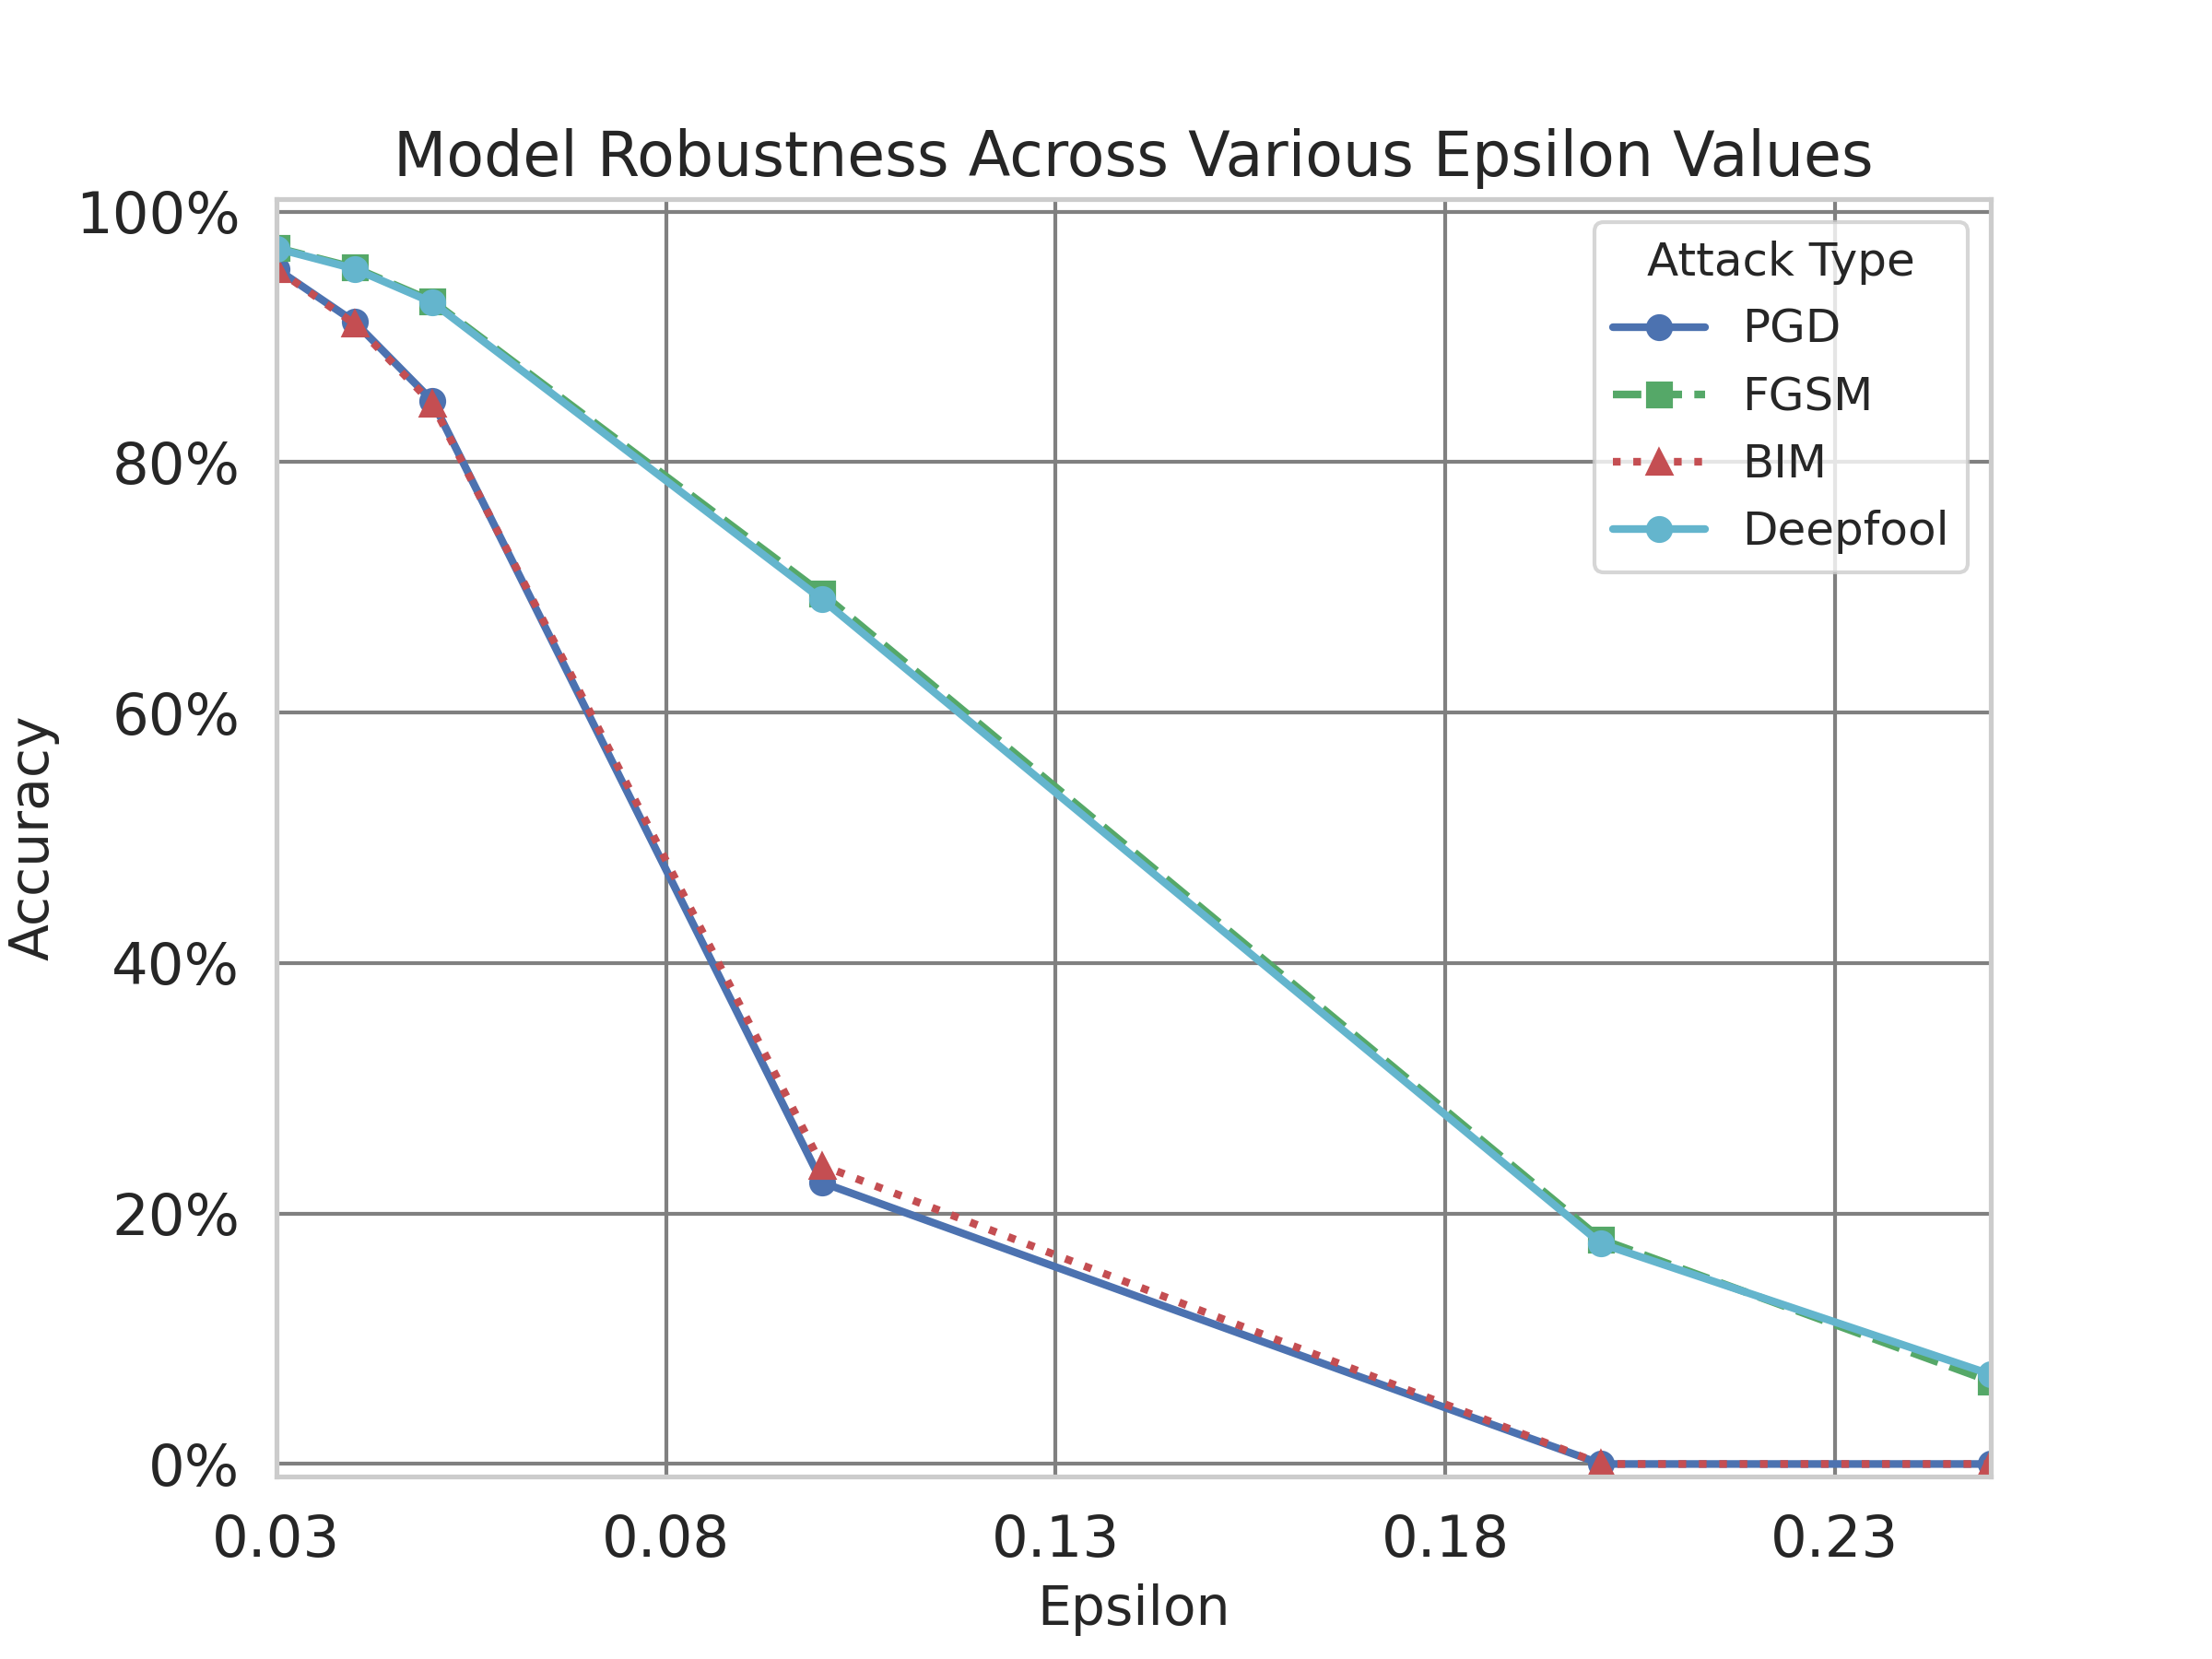
\includegraphics[width=\linewidth]{paper_images/Result1.png}
%     \caption{Assessing Model Robustness Across Various Epsilon Values Under Four Types of Attacks}
%     \label{fig:robust_accuracy_attacks}
% \end{figure}

% \begin{table}[ht]
%     \centering
%     \caption{Summary of Total Misclassifications for Various Adversarial Attacks}
%     \label{tab:misclassifications}
%     \begin{tabular}{|l|c|c|c|c|c|c|}
%     \hline
%     & \multicolumn{6}{c|}{\textbf{Epsilon}} \\ \cline{2-7} 
%     \multirow{-2}{*}{\textbf{Attack Type}} & \textbf{0.03} & \textbf{0.04} & \textbf{0.05} & \textbf{0.10} & \textbf{0.20} & \textbf{0.25} \\ \hline
%     BIM & 451 & 881 & 1508 & 7490 & 9834 & 9834 \\ \hline
%     FGSM & 284 & 440 & 702 & 2998 & 8070 & 9186 \\ \hline
%     Deepfool & 289 & 449 & 713 & 3045 & 8104 & 9130 \\ \hline
%     PGD & 451 & 881 & 1483 & 7616 & 9834 & 9834 \\ \hline
%     \end{tabular}
% \end{table}

The findings emphasize the importance of implementing advanced defensive measures to enhance the robustness of machine learning models against 
adversarial attacks. The observations made in this case study can help in the creation of such defenses, especially in addressing the weaknesses exposed by BIM and PGD when dealing with smaller perturbations, and the slower but eventual impact of FGSM and DeepFool when dealing with higher perturbations.


\subsection{Pixel-Level Analysis using Gradient Explainer}
 
  This case study delves into a novel approach to bolster model robustness, integrating SHAP (SHapley Additive exPlanations) analysis with pixel categorization and manipulation. Unlike traditional applications of SHAP, our methodology ventures into pixel categorization, critical pixel thresholds, and their impact on model resilience. We investigate the interplay between critical pixels and model accuracy under adversarial challenges, focusing on scenarios where the model's performance is compromised. By employing 200 samples for each adversarial attack and correct image across six epsilon values, we evaluate over tens of thousands of data points. Our findings shed light on the intricate dynamics between critical pixels and model robustness, presenting new avenues for enhancing deep learning model defenses against adversarial attacks.

  In response to this growing concern, our case study explores an innovative approach to bolster model robustness. While SHAP analysis and SHAP signatures have been pivotal in model explanation and enhancement, our study extends these concepts to encompass pixel categorization and manipulation. We introduce the concept of "critical pixels" those that exert a profound influence on model predictions. By setting critical pixel thresholds, we aim to achieve precision levels exceeding 70\%, 80\%, or 90\% within the SHAP signature.

  Our experimental design encompasses both normal and adversarial images, comprising 200 samples for each attack and correct image across six epsilon values. This meticulous dataset design allows for a comprehensive evaluation of model behavior under varying adversarial conditions. Notably, we exclusively select adversarial examples that confound the model, ensuring our focus on scenarios where model accuracy is compromised.
  
  The results of our study reveal the intricate relationship between critical pixels and model robustness. By modifying critical pixels in adversarial images, we investigate whether such alterations can resuscitate model accuracy. Simultaneously, we analyze the impact of critical pixel modifications in regular images, exploring whether such changes detrimentally affect model accuracy.
  
  Our findings suggest that critical pixels indeed play a pivotal role in influencing model behavior under adversarial conditions. The interplay between these critical pixels and model robustness is nuanced, with critical pixel manipulation serving as a potential avenue for model defense. However, our study also underscores the delicate balance between critical pixel alterations and model performance in regular images, revealing the need for a nuanced approach to model enhancement.
  
%   \begin{figure}
%     \centering
%     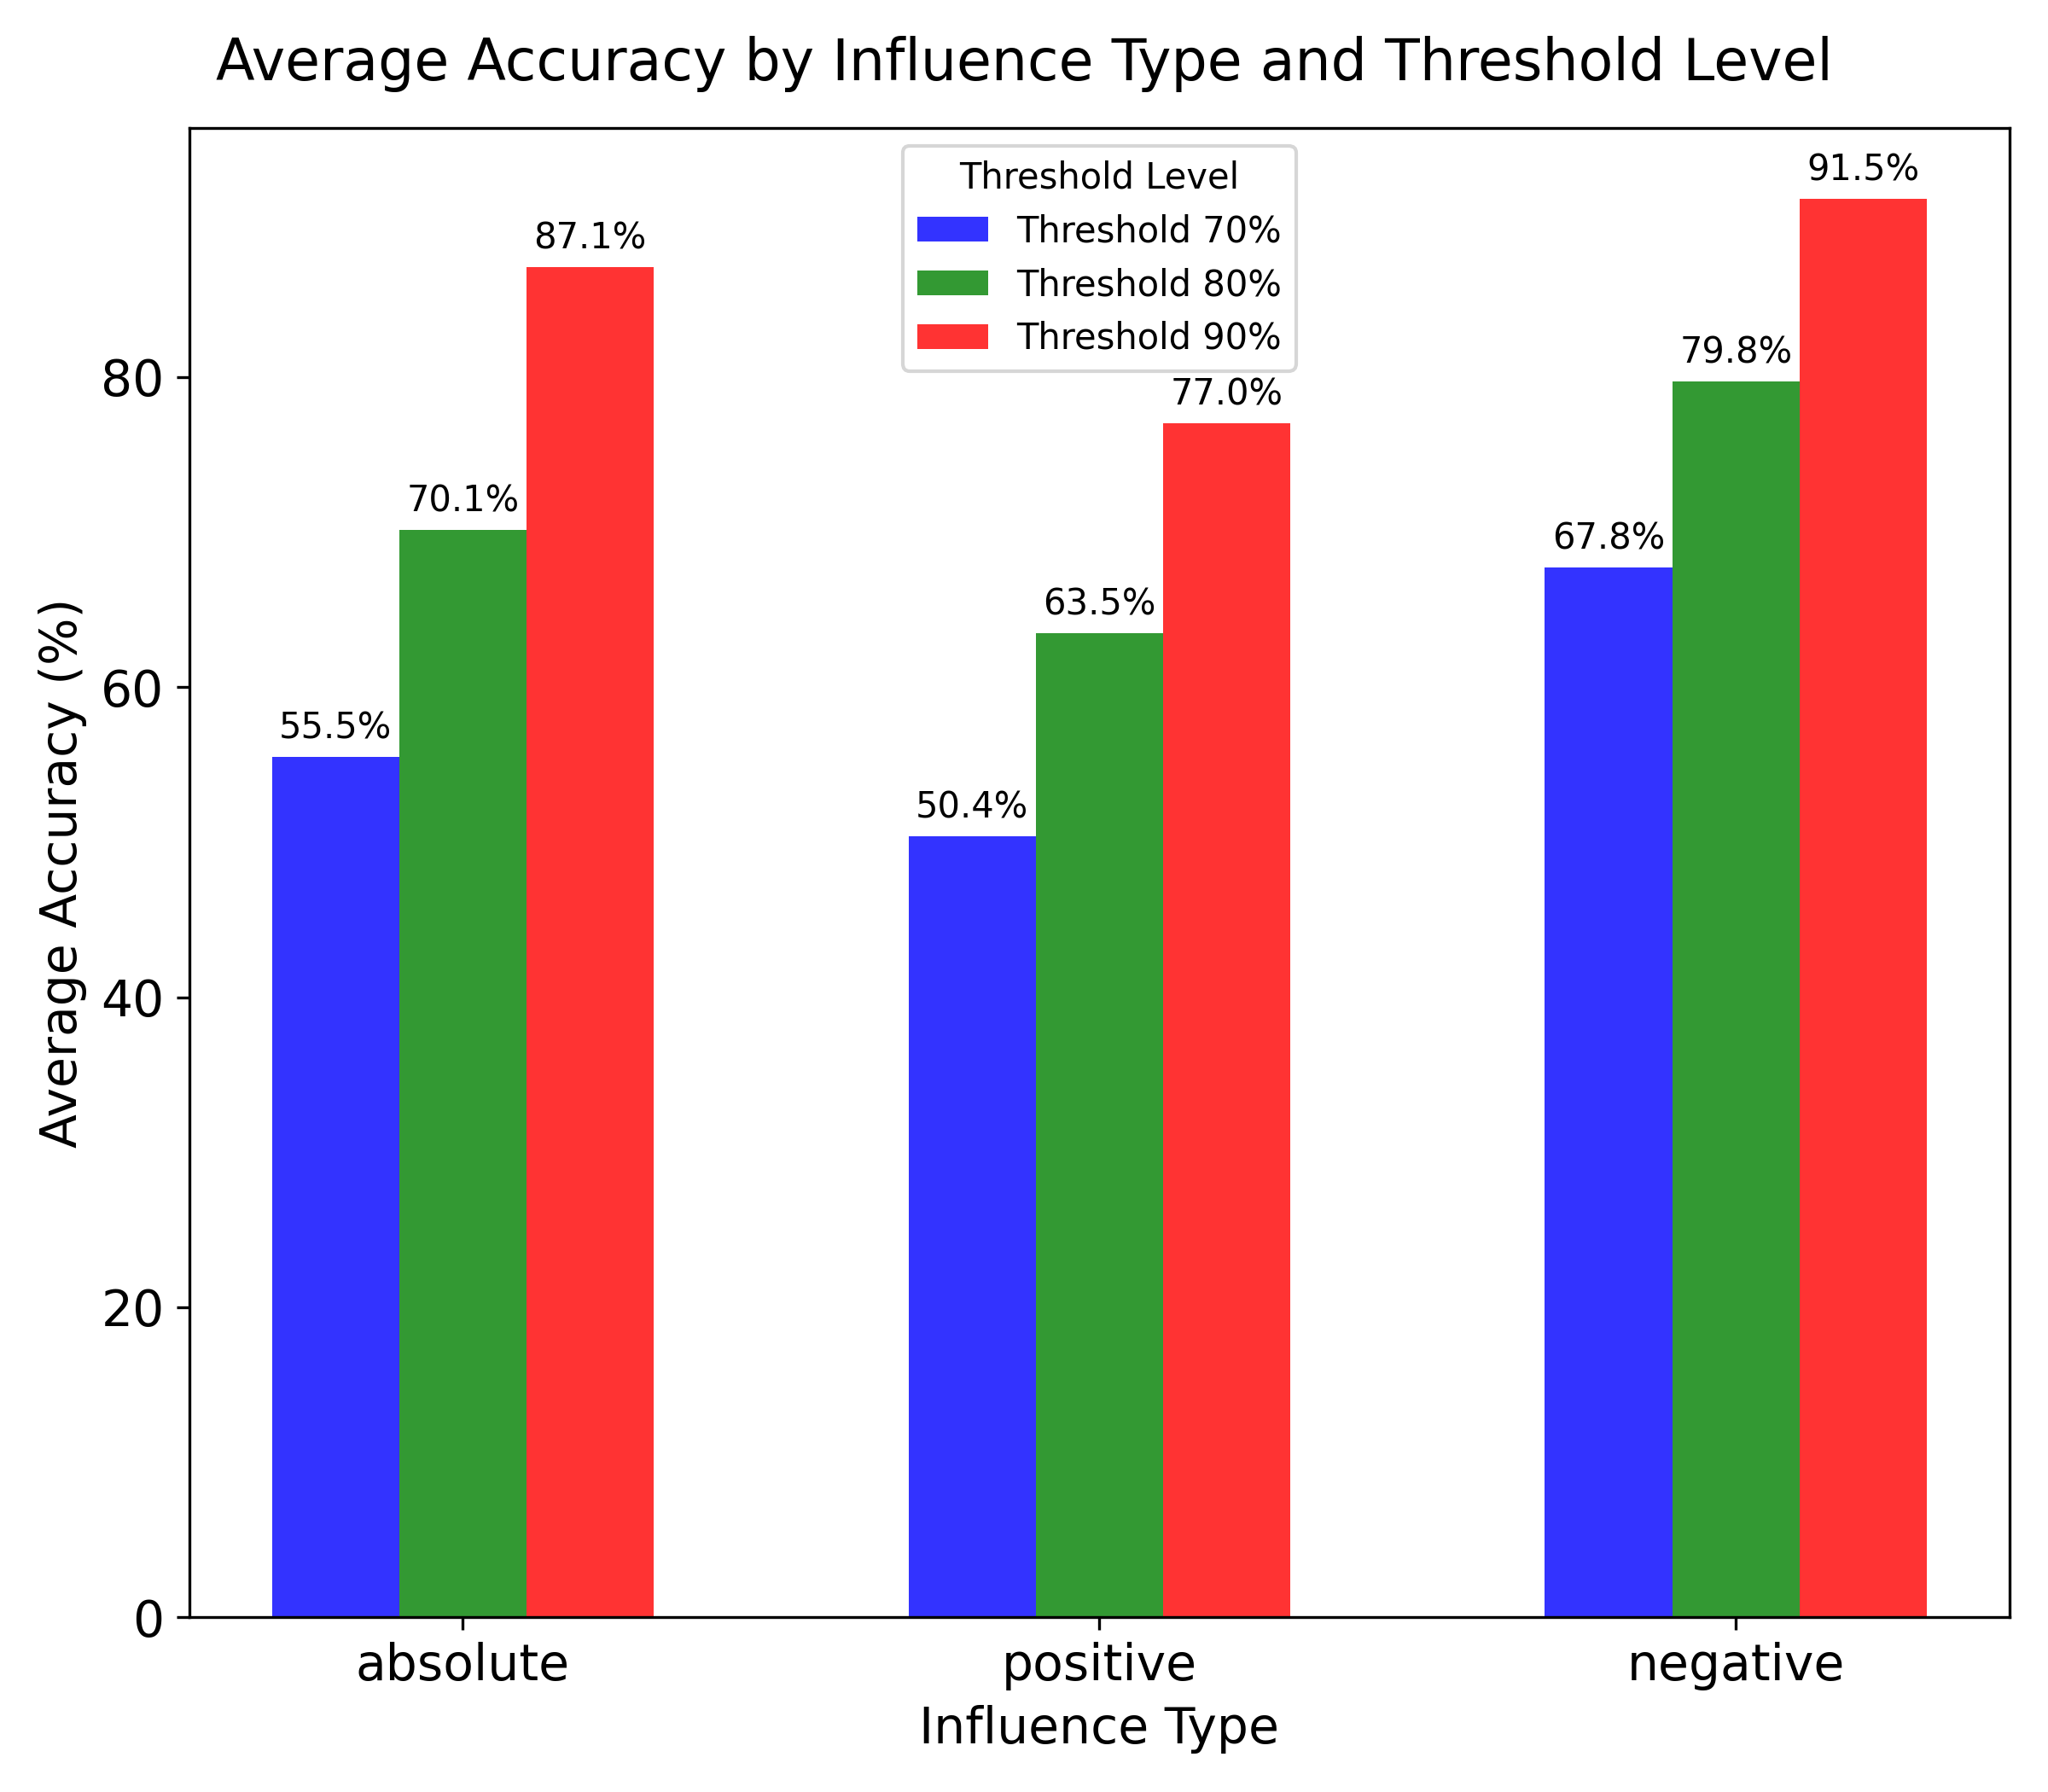
\includegraphics[width=0.9\linewidth]{paper_images/correctinf.png}
%     \caption{Degradation of Model Accuracy with Increased Critical Pixel Thresholds on Normal Images}
%     \label{Degradation}
% \end{figure}
%   \begin{figure*}
%     \centering
%     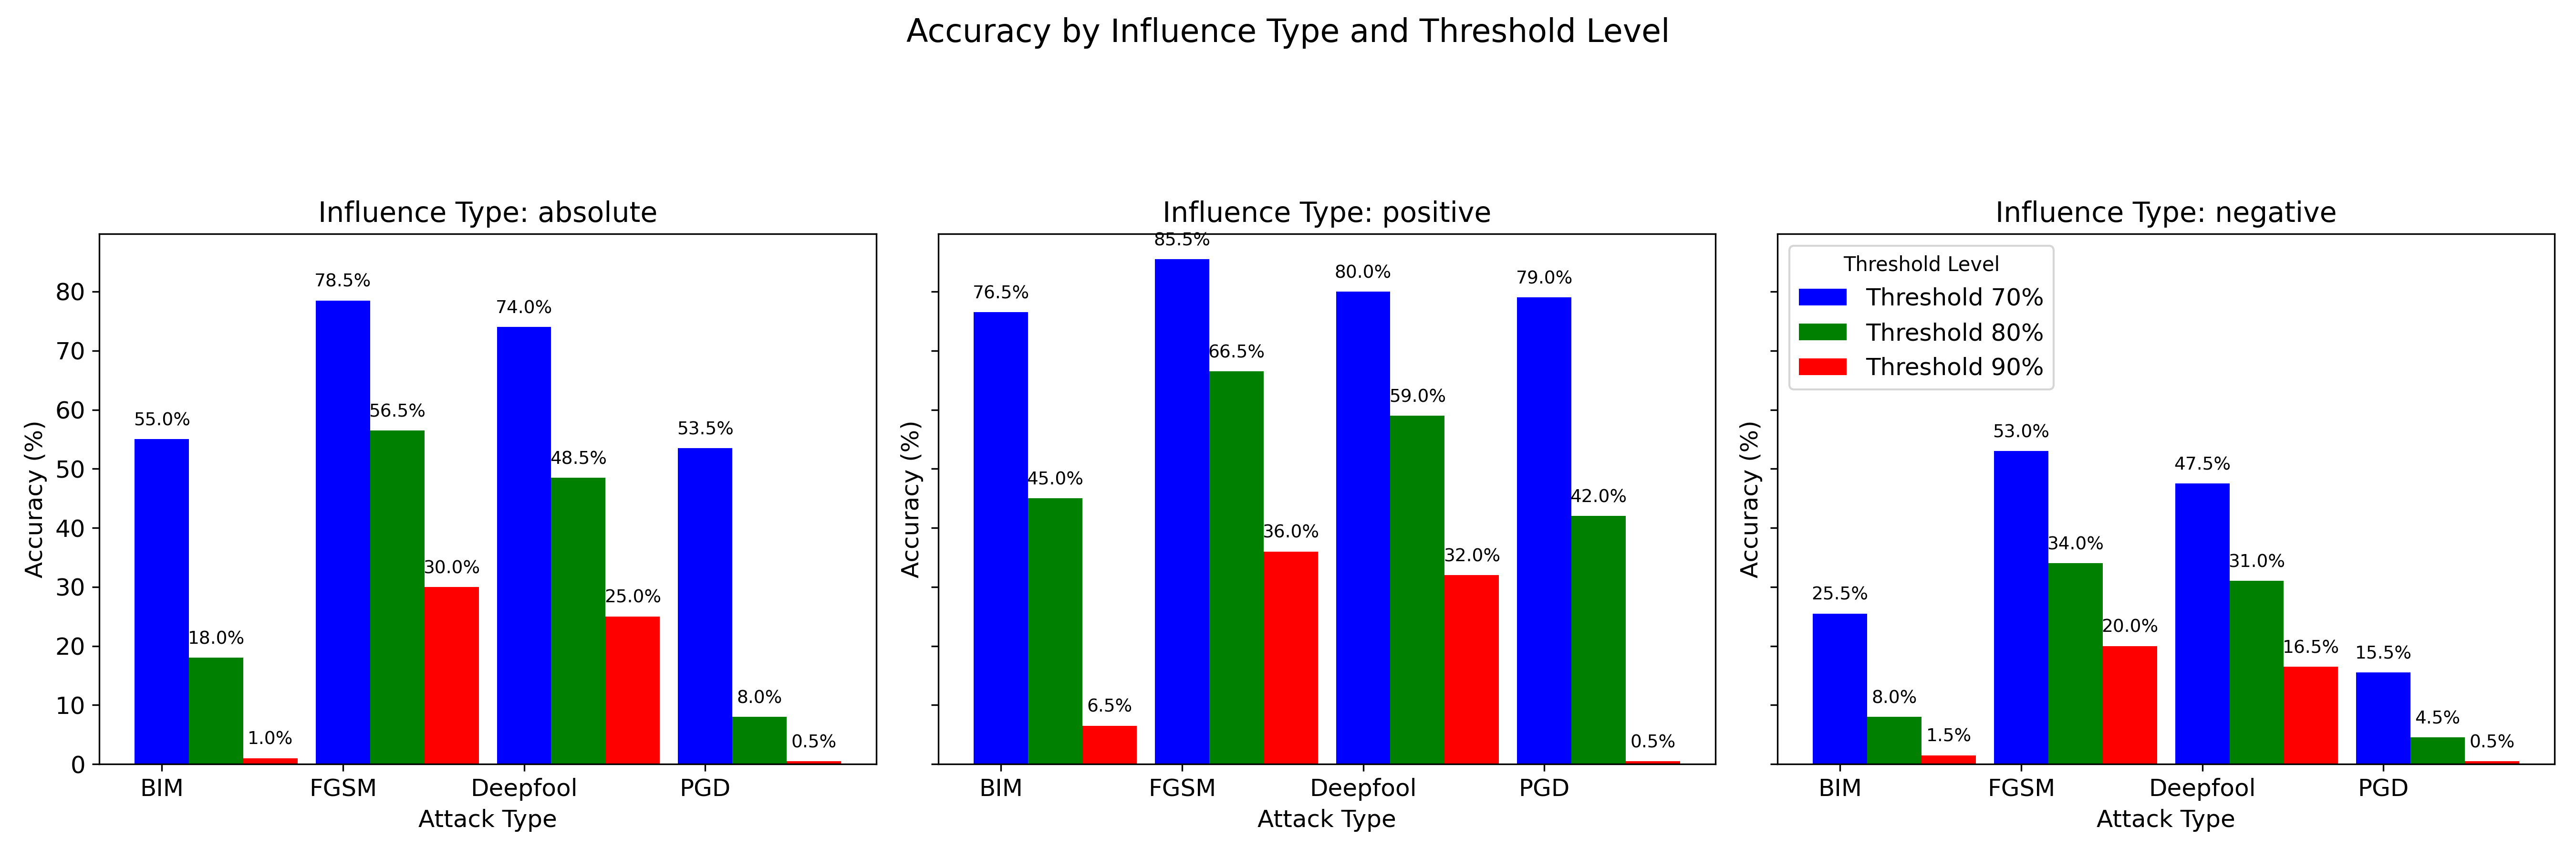
\includegraphics[width=\linewidth]{paper_images/critical_adv.png}
%     \caption{Recovery of Model Accuracy through Critical Pixel Manipulation in Adversarial Images (Epsilon = 0.25)}
%     \label{Recovery}
% \end{figure*}

% \begin{figure}[ht]
%     \centering
%     \begin{minipage}{0.25\textwidth}
%         \centering
%         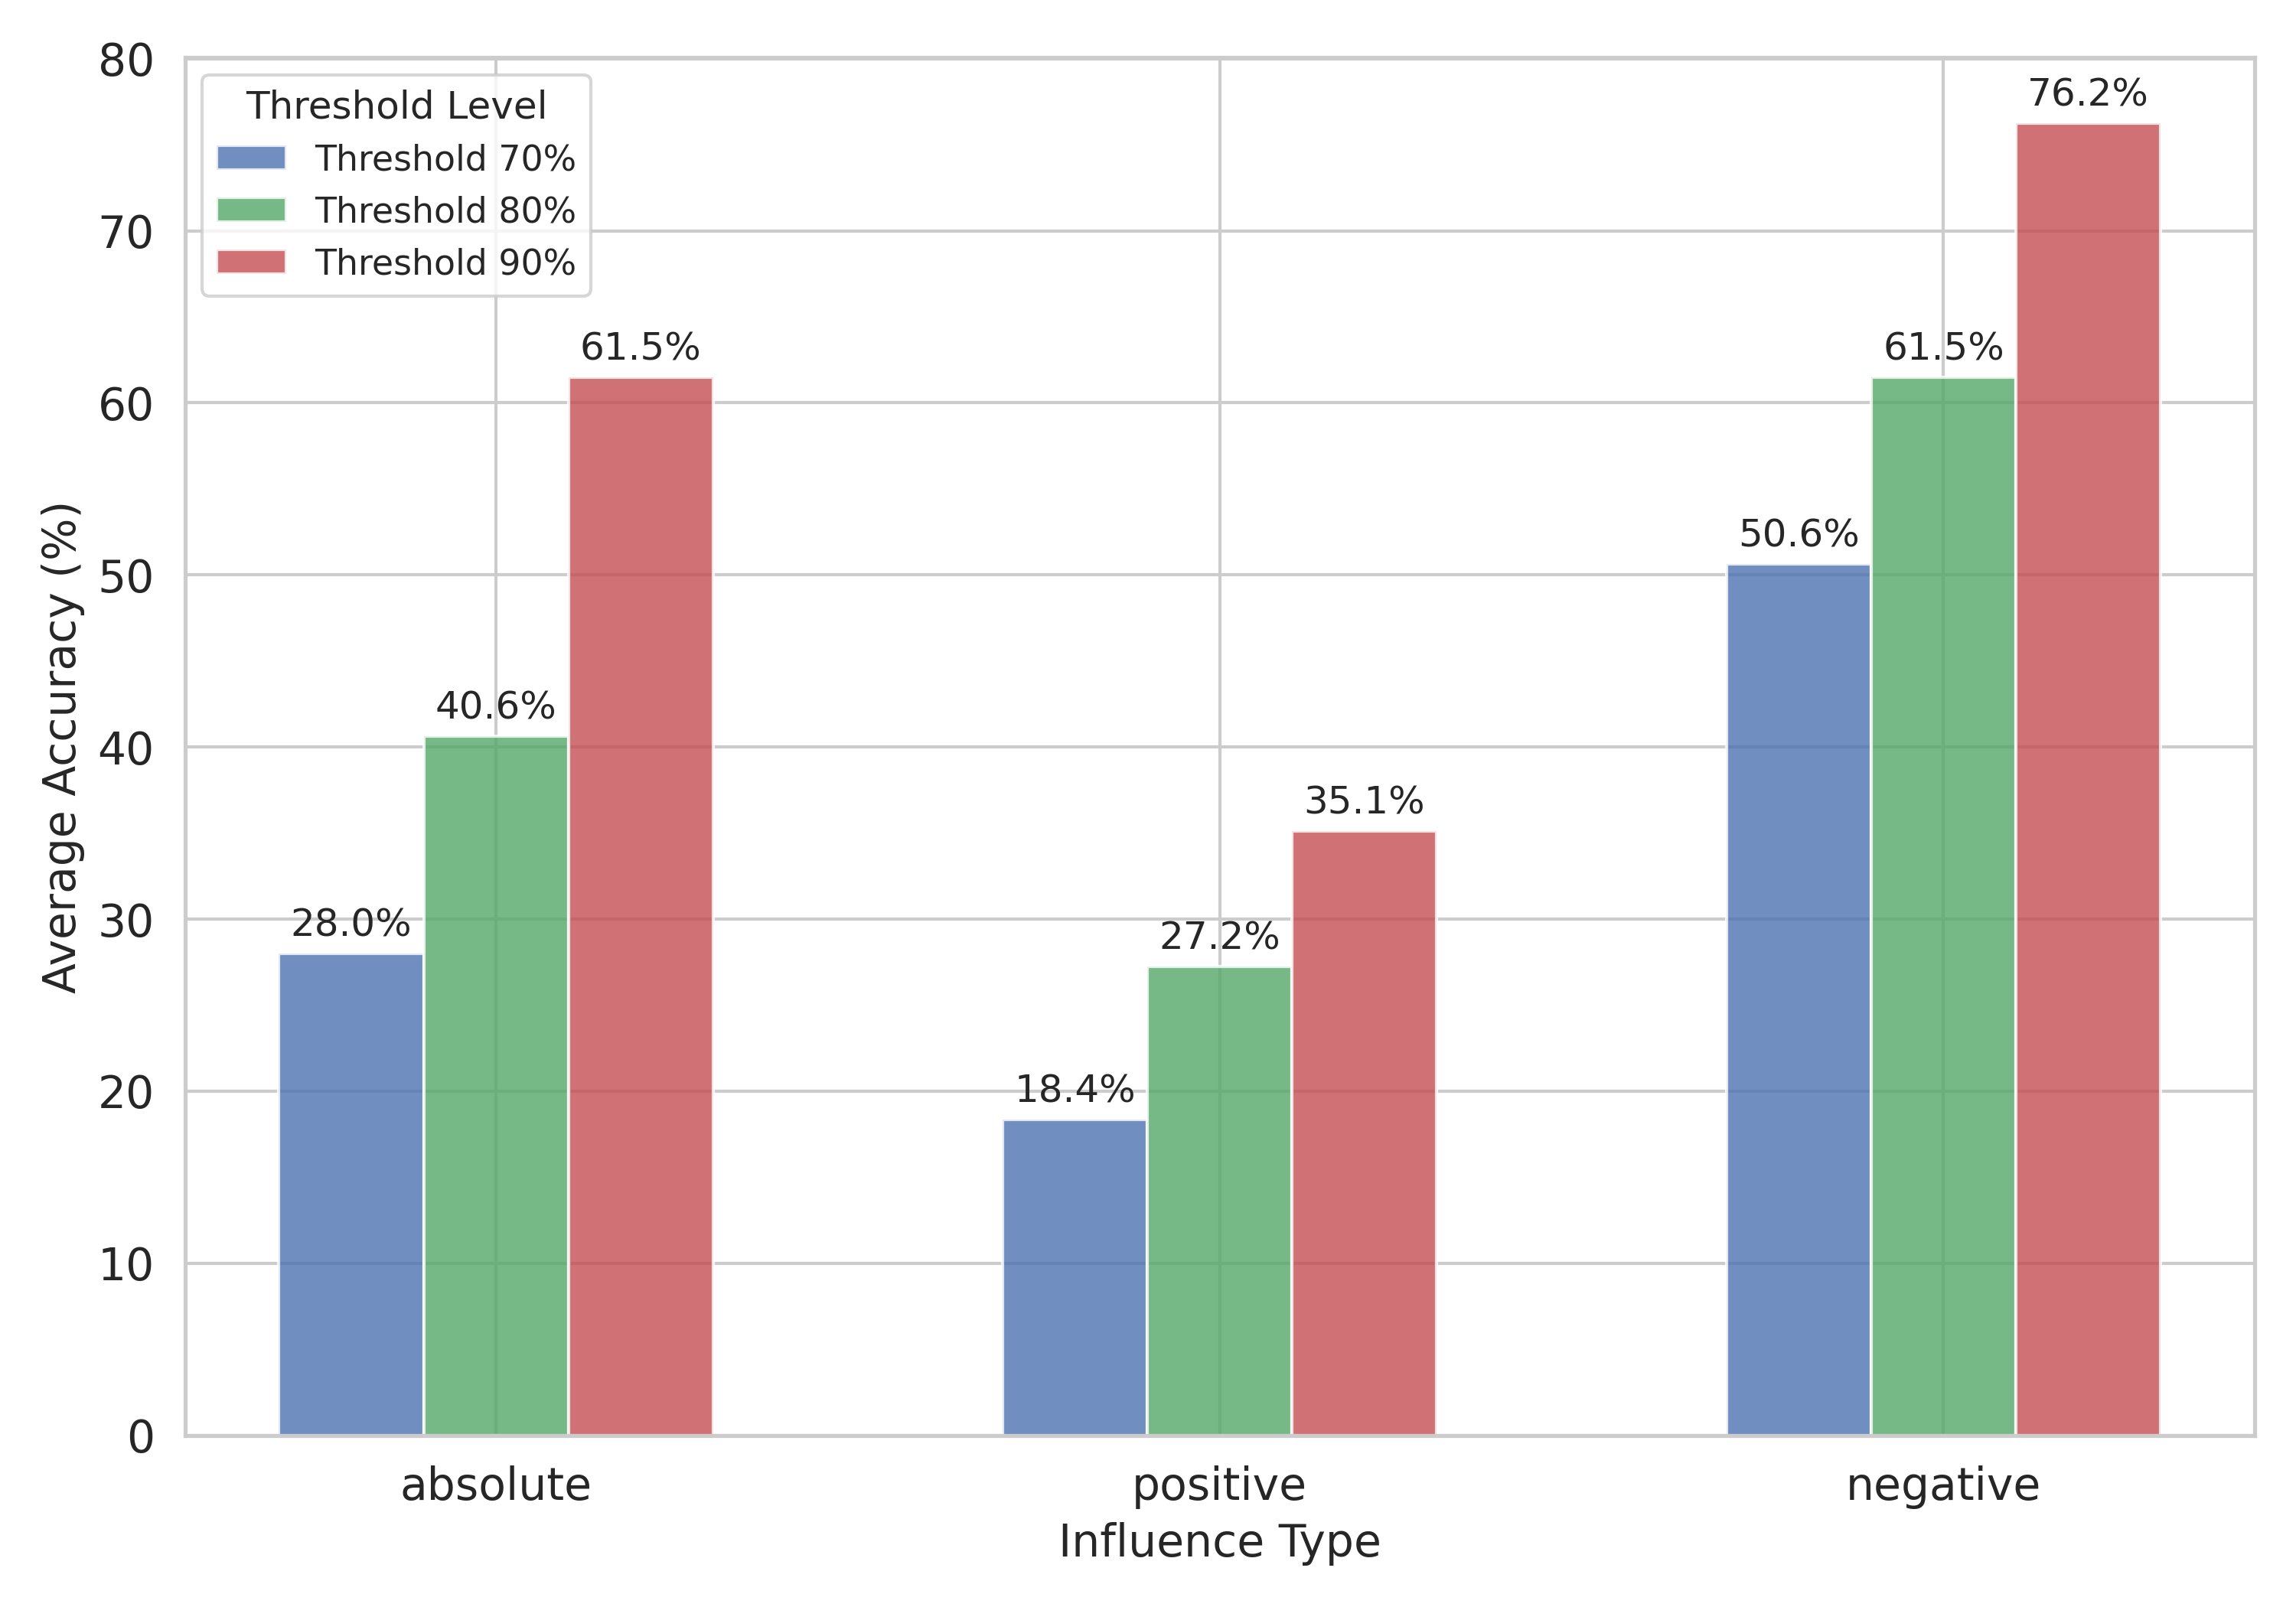
\includegraphics[width=\linewidth]{deepexplainer/correctinf.png}
%         \caption{Pixel Importance Deep}
%     \end{minipage}\hfill
%     \begin{minipage}{0.25\textwidth}
%         \centering
%         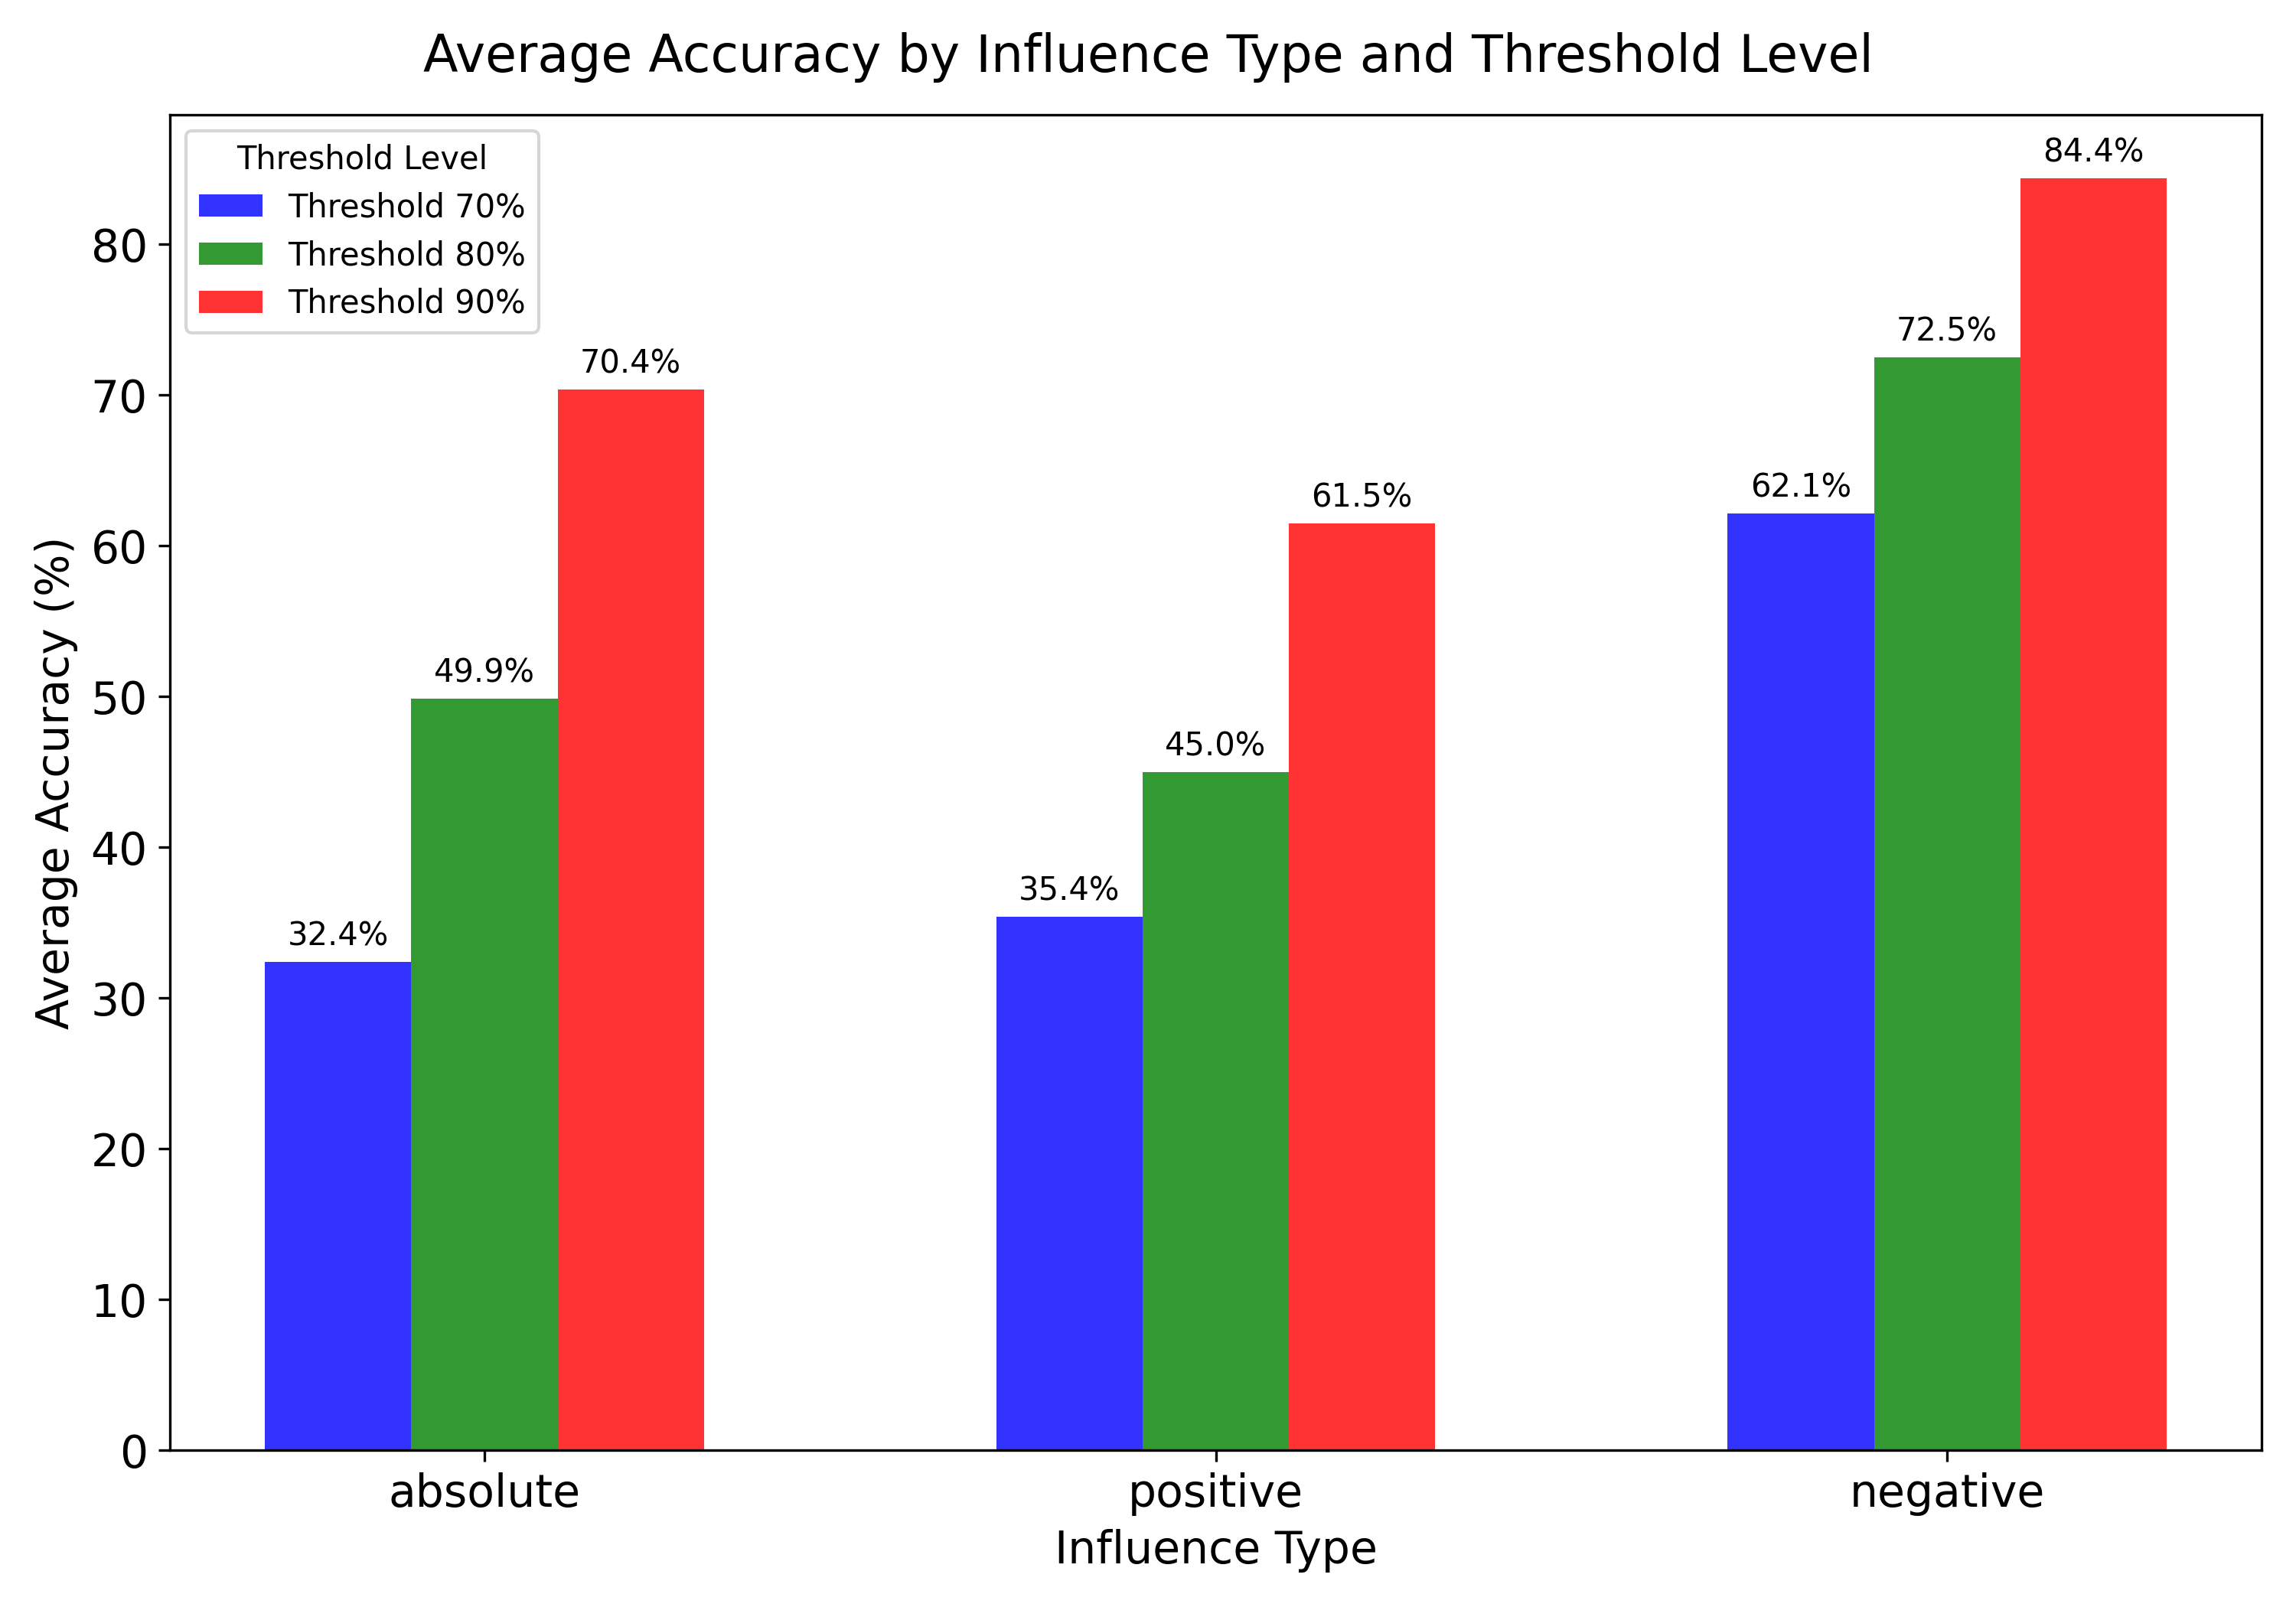
\includegraphics[width=\linewidth]{gradient/correctinf.png}
%         \caption{Pixel Importance Gradient}
%     \end{minipage}
% \end{figure}

  \begin{figure}
    \centering
    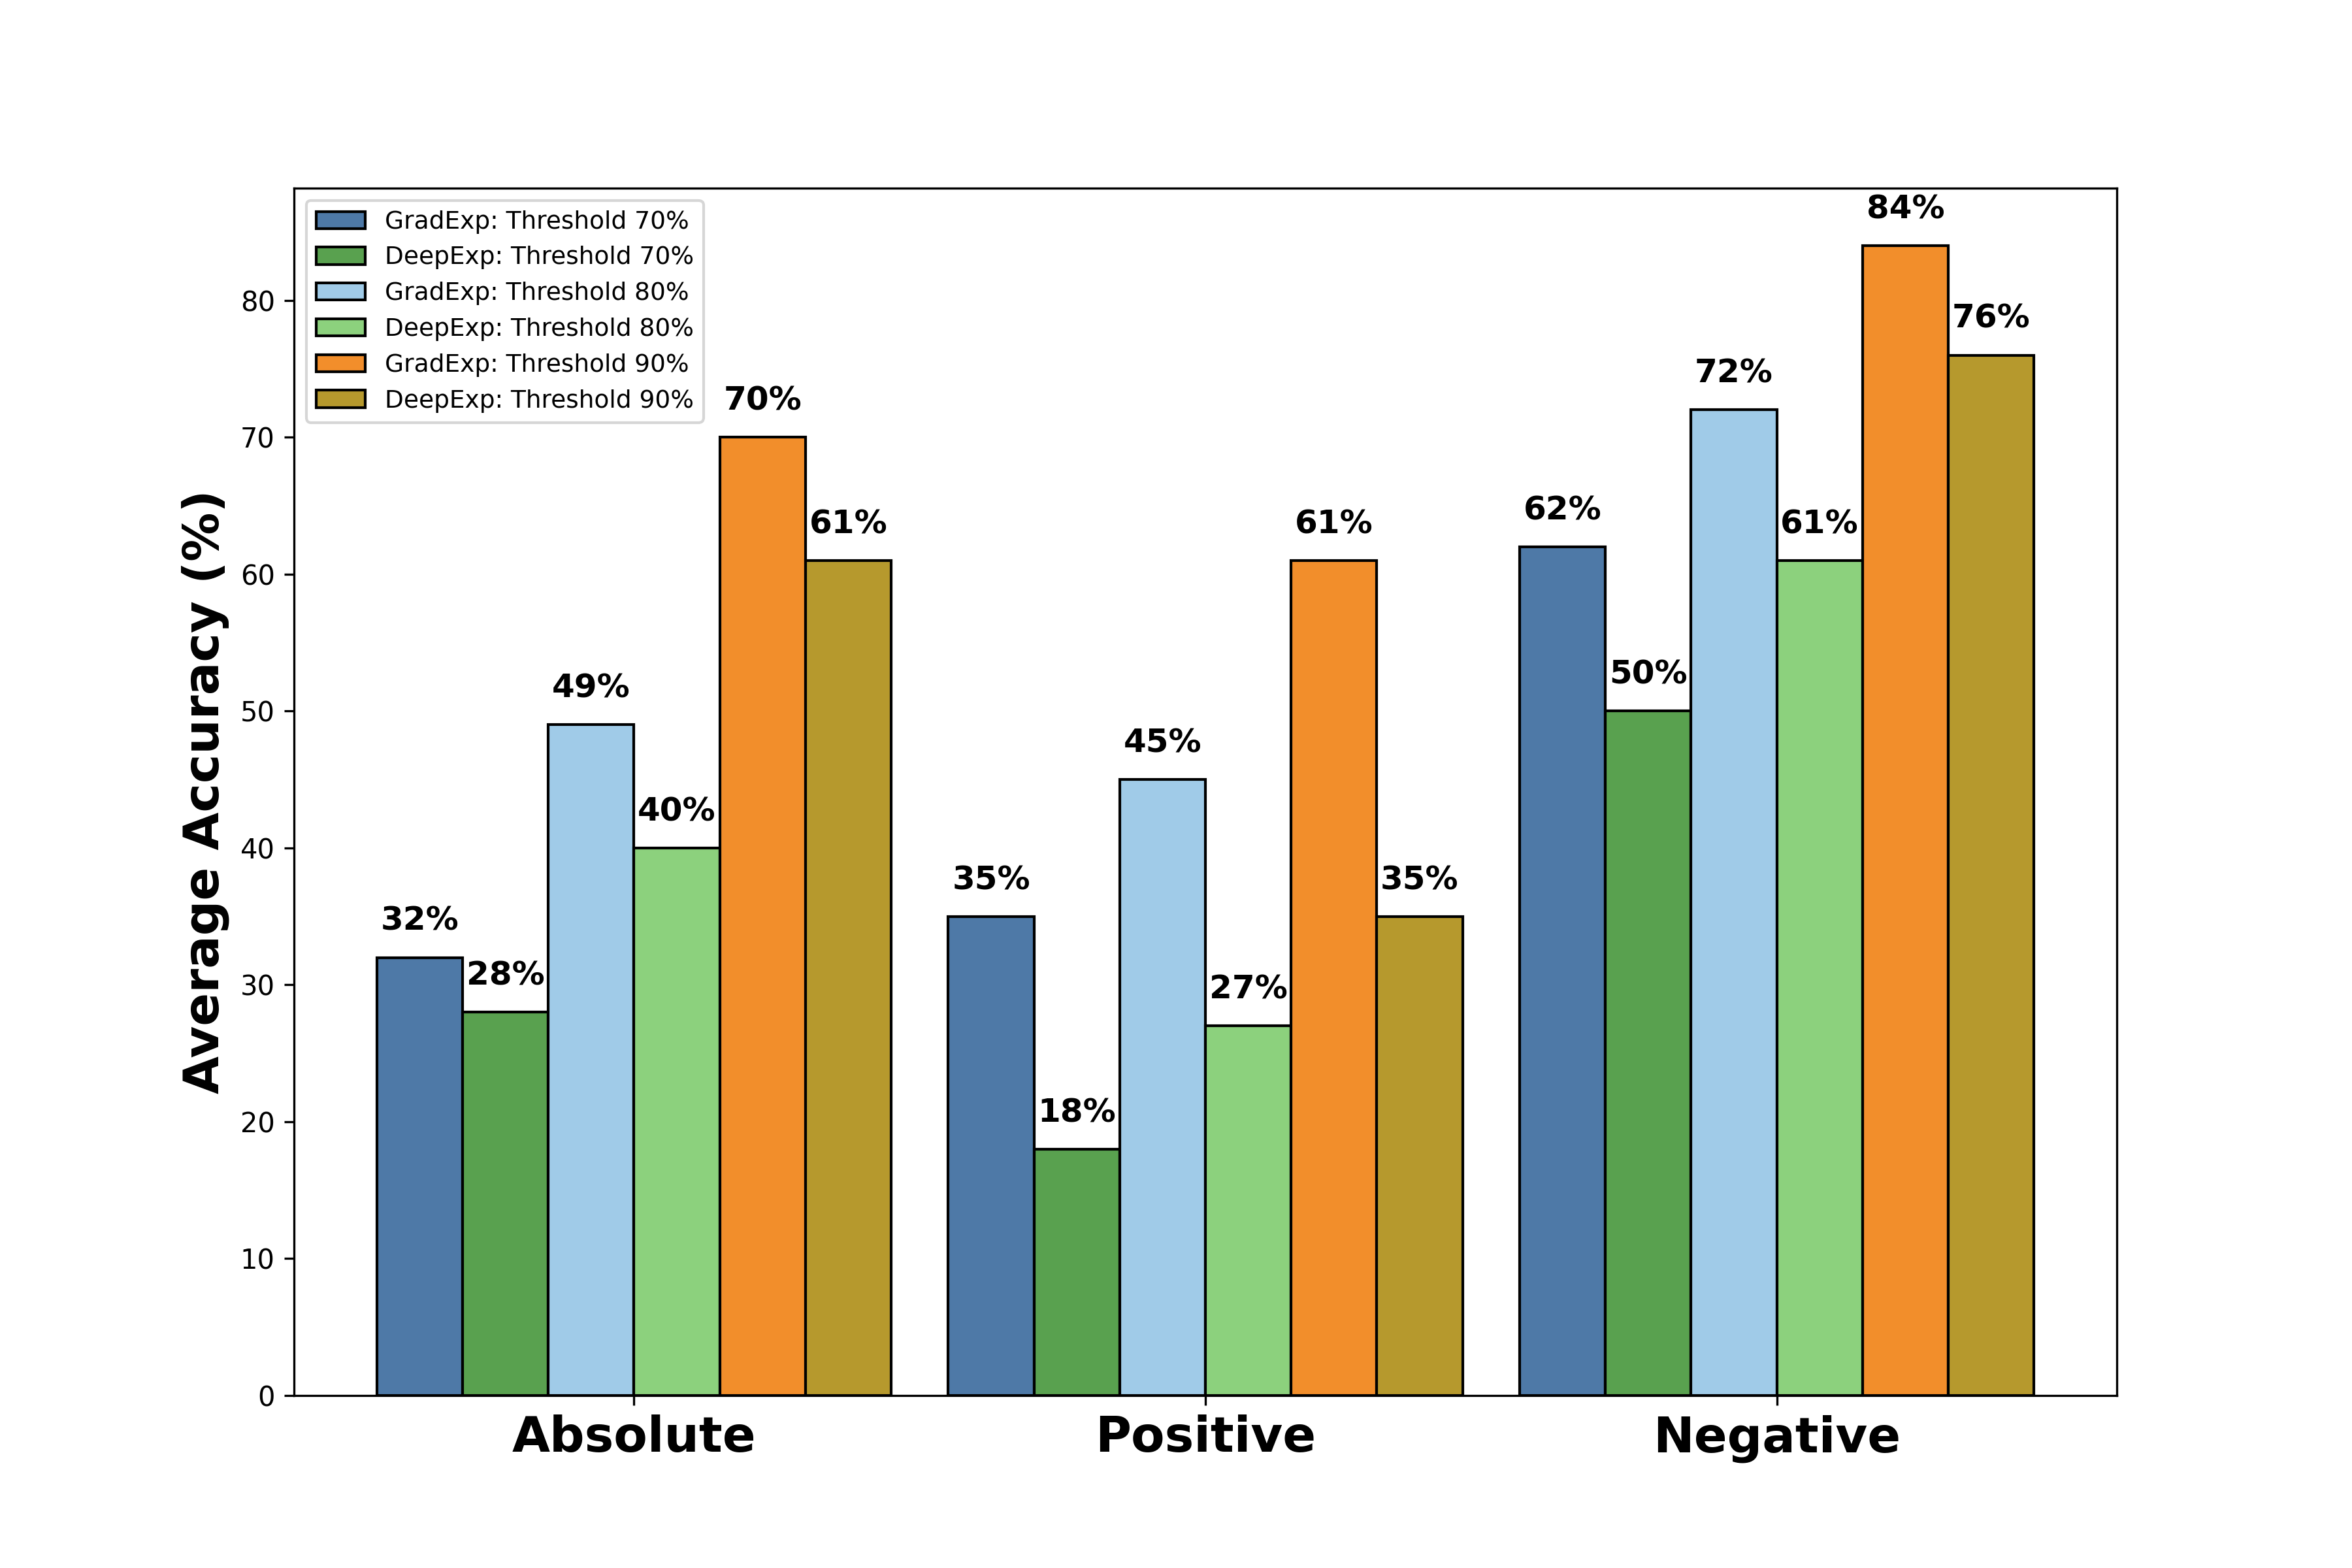
\includegraphics[width=1\linewidth]{comapre_explainer/correctgradanddeep.png}
    \caption{Represents the impact on model accuracy when modifying normal image pixels based on different levels of influence and thresholds. The expectation is that the accuracy would decrease from 100\% as critical pixels are altered}
    \label{Degradation}
\end{figure}

\begin{figure*}[ht]
    \centering
    \begin{minipage}{1\textwidth}
        \centering
        \includegraphics[width=\linewidth]{comapre_explainer/advgradanddeep_70.png}
        \caption{Pixel Importance Deep}
    \end{minipage}\hfill
    \begin{minipage}{1\textwidth}
        \centering
        \includegraphics[width=\linewidth]{comapre_explainer/advgradanddeep_80.png}
        \caption{Pixel Importance Deep}
    \end{minipage}\hfill
    \begin{minipage}{1\textwidth}
        \centering
        \includegraphics[width=\linewidth]{comapre_explainer/advgradanddeep_90.png}
        \caption{Pixel Importance Gradient}
    \end{minipage}
\end{figure*}




Figure.\ref{Degradation} represents the impact on model accuracy when modifying normal image pixels based on different levels of influence and thresholds. The expectation is that the accuracy would decrease from 100\% as critical pixels are altered.
Figure.\ref{Recovery} represents the impact on model accuracy when modifying adversarial image pixels to restore accuracy. The plot specifically deals with adversarial examples generated with an epsilon value of 0.25, and the goal is to observe how the accuracy increases from 0\% upwards.
 
In Figure.\ref{Degradation}, the observed trend is an expected decrease in model accuracy as the threshold for critical pixel influence increases. This decrease is pronounced within the 'absolute' influence type, suggesting that indiscriminate alteration of pixels deemed critical—without considering the nature of their influence—can significantly degrade model performance. Notably, the transition from the 80\% to the 90\% threshold underscores the sensitivity of the model to pixel-level changes, particularly for pixels with a 'positive' influence, which seems to play a substantial role in maintaining the model's high accuracy on standard images.

Figure.\ref{Recovery} offers insights into the recovery of accuracy for adversarial images by modifying critical pixels, with an emphasis on samples generated with an epsilon value of 0.25. The model's response to pixel manipulation varies across different attack types, which implies that the efficacy of such defensive measures is contingent on the attack's characteristics. It's particularly interesting that for the 'absolute' influence type, a broader definition of critical pixels (as seen at the 70\% threshold) aids in mitigating the effects of simpler attacks like BIM and FGSM. However, for more complex attacks such as Deepfool and PGD, even high precision in identifying critical pixels does not significantly bolster the model's resilience.

These plots collectively underscore the complexity inherent in enhancing model robustness through pixel manipulation. While adjusting critical pixels shows promise as a line of defense, its success is clearly attack-dependent. The findings advocate for a strategic approach to applying SHAP-based pixel modifications, where the type of pixel influence—be it absolute, positive, or negative—must be carefully considered to avoid diminishing model accuracy or failing to recover it in the face of adversarial challenges.

The case study, therefore, highlights the importance of a multifaceted defense strategy that incorporates pixel-level interventions alongside other techniques to construct a robust defense against a spectrum of adversarial strategies. Given that the analysis is based on a fixed epsilon value, further research should encompass a wider array of attack intensities to ensure broader applicability and resilience of the proposed defense mechanisms.
  

  \subsection{Case Study 3: Validation of Identified Critical Pixels}
    In Section VI, we discussed the critical pixels identified through our methodology for both attack generation and detection. To determine their significance, we conducted a rigorous statistical validation using a two-sample t-test. This validation step is crucial to highlight the critical role played by these pixels in shaping the decision-making process of our machine learning model.

    Our approach involved a comprehensive examination of SHAP values, with specific emphasis on those related to attack detection. SHAP values are useful in understanding the inner workings of our model, and they shed light on the pixels that significantly influence its predictions. To streamline the analysis, we categorized these SHAP values into two distinct groups: critical pixels and non-critical pixels. We based this categorization on a set of indices derived from our methodology.
    Figure \ref{fig:bar_chart} displays a bar chart that compares the means of two groups, highlighting the difference in mean SHAP values for 'Critical' and 'Non-Critical' pixels. This visual representation is critical to our analysis.   
    Figure \ref{fig:histograms} shows histograms of SHAP values that provide a closer look at the distribution of SHAP values for both 'Critical' and 'Non-Critical' pixels. These histograms help us to understand the data distribution and its impact on statistical tests.    
    The validation of our study primarily depends on the comparison of two groups using statistical analysis. We used the two-sample t-test, a well-known method for identifying significant differences between two sets of data. Our results were significant with a computed t-statistic of 11.5968 and an extremely low p-value of $1.34 \times 10^{-30}$. Figures \ref{fig:bar_chart} and \ref{fig:histograms} show the statistical indicators that confirm the crucial role of critical pixels in our model's behavior. These pixels influence both the generation and detection of adversarial attacks.
    
 
        \begin{figure}
            \centering
            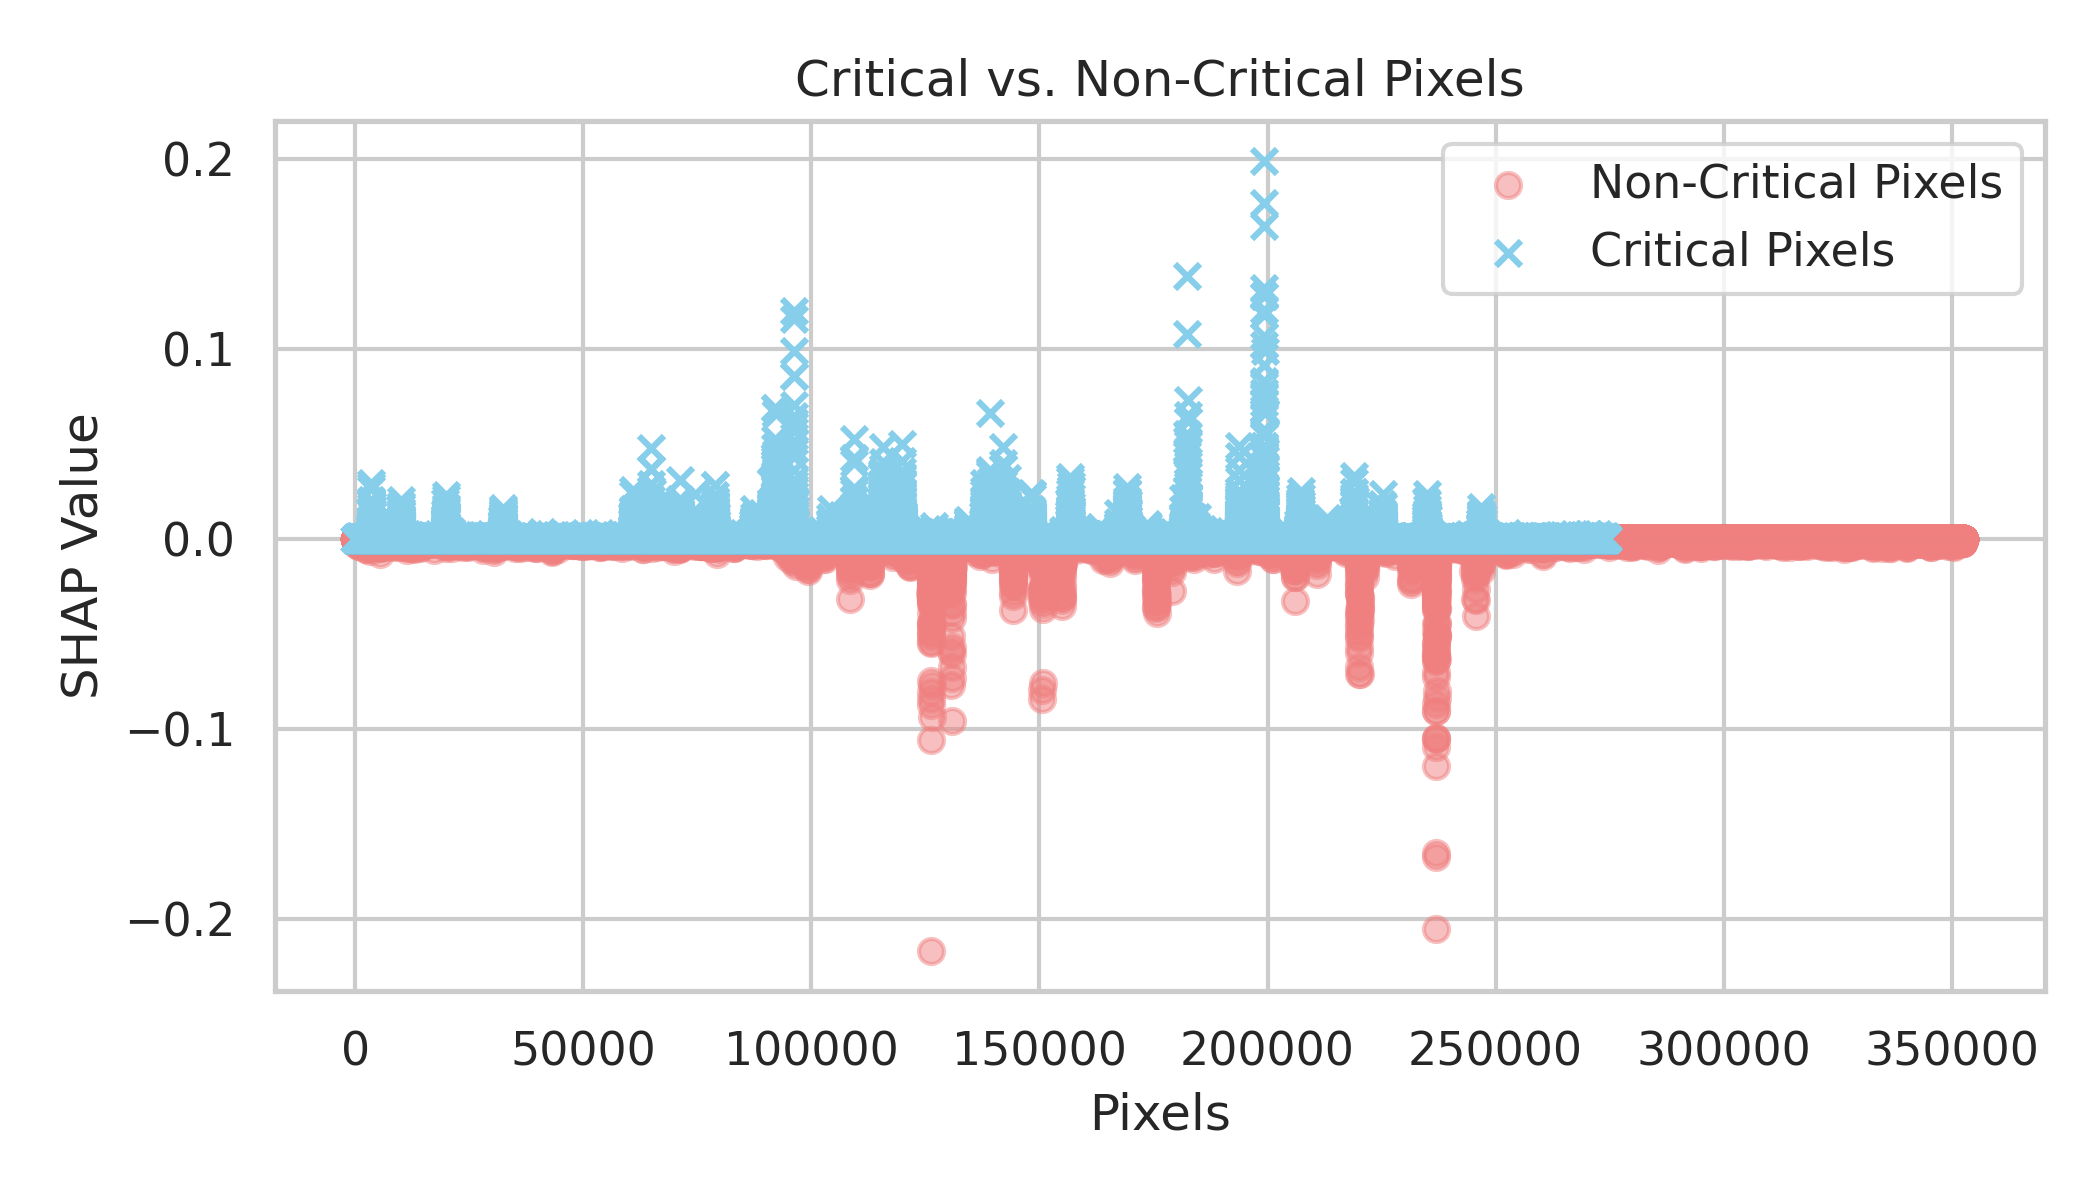
\includegraphics[width=0.9\linewidth]{deepexplainer/ttest.png}
            \caption{Pixel Importance Deep}
        \end{figure}
     
        \begin{figure}
            \centering
            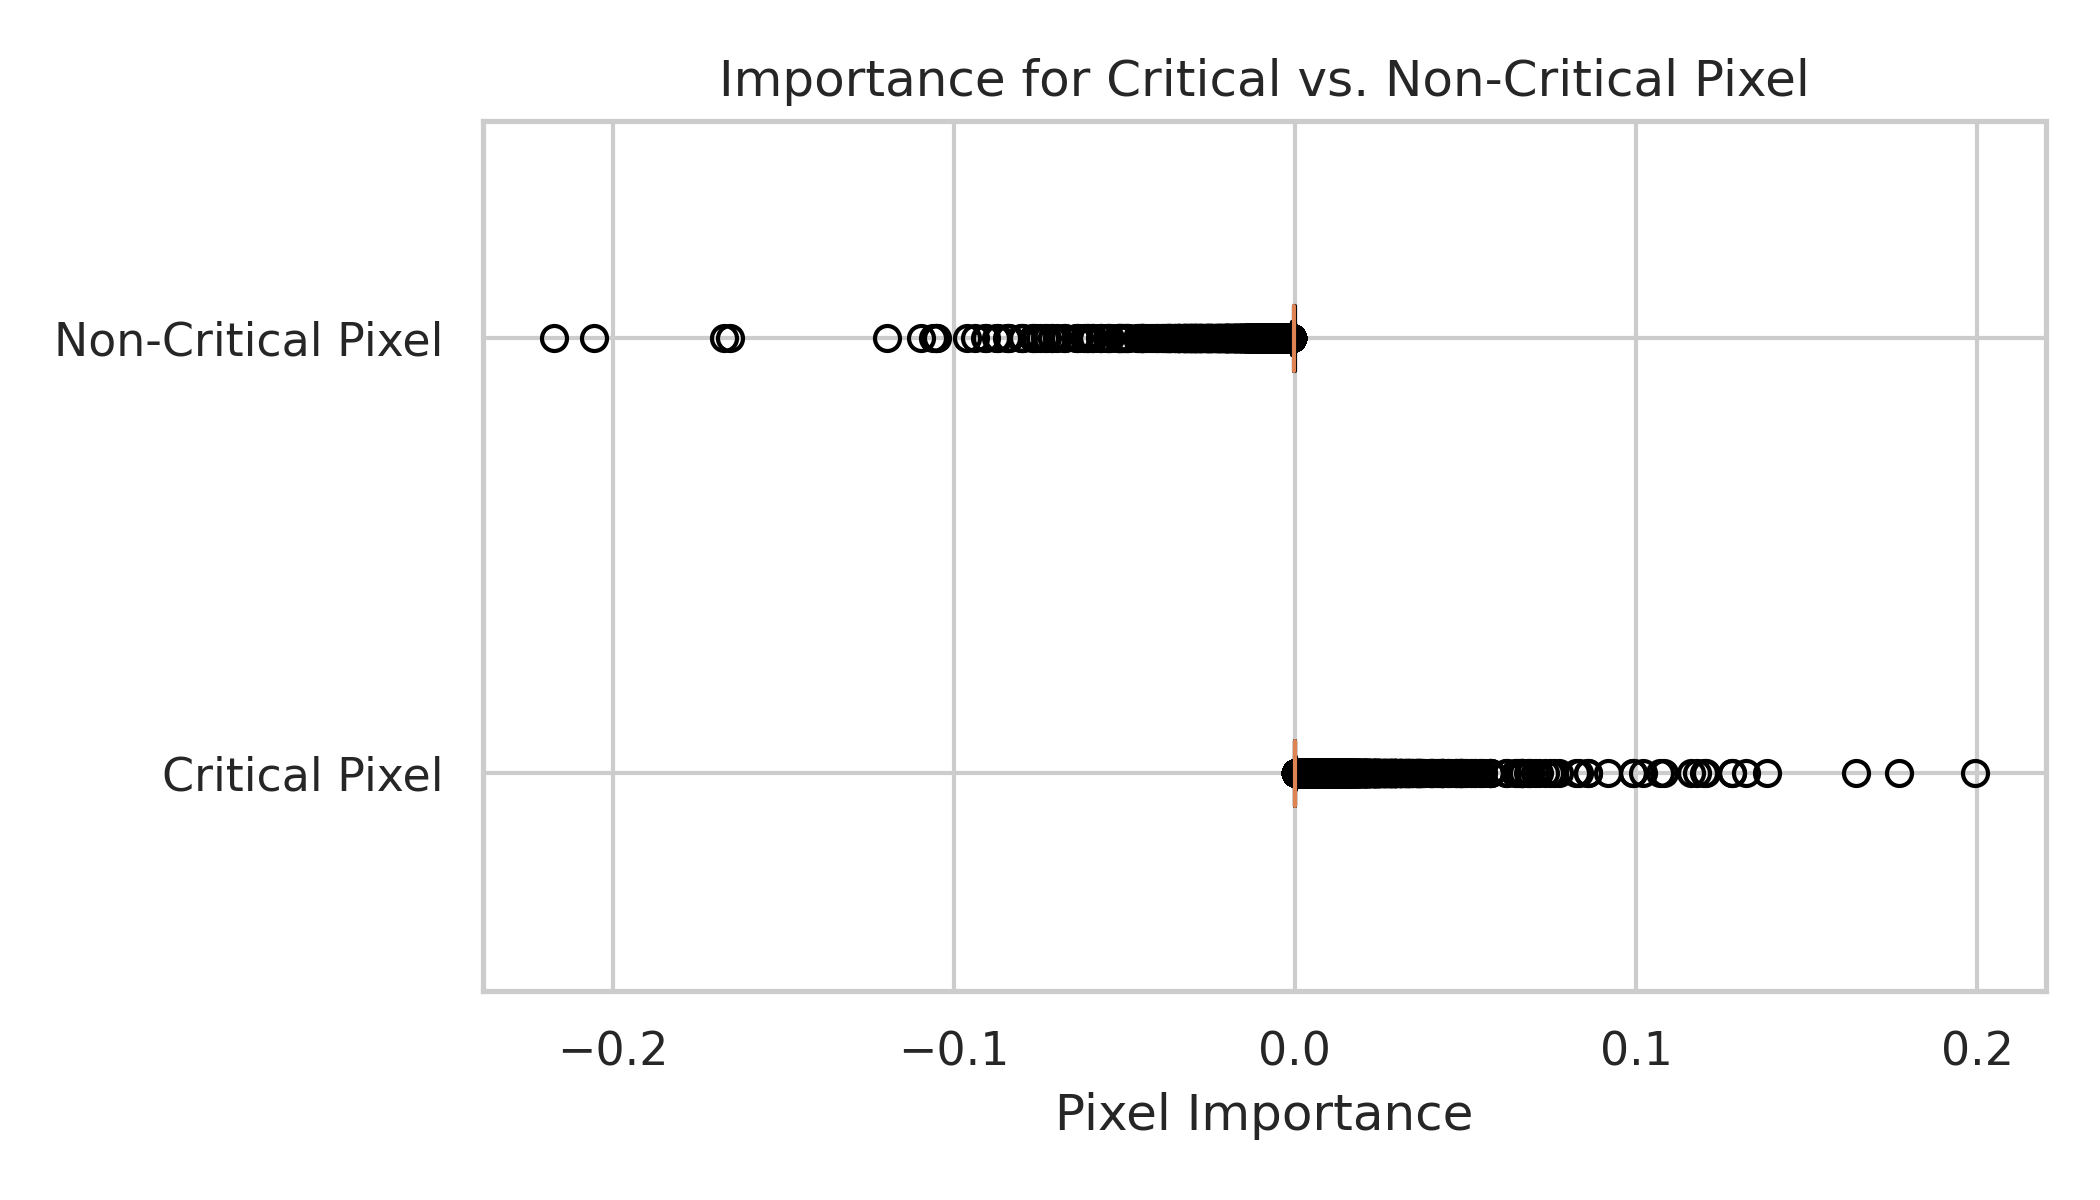
\includegraphics[width=0.9\linewidth]{deepexplainer/ttest2.png}
            \caption{Pixel Importance Deep}
        \end{figure}

        
% \section{Future Directions}

% By leveraging our pixel-level analysis methodology, we have identified several critical areas for future research that can extend and enhance our understanding of AI's robustness and interpretability:

% \noindent \textbf{Complex and High-Dimensional Datasets:}
% \begin{itemize}
%     \item To test the scalability and adaptability of our approach in more complex scenarios than MNIST, future research should concentrate on utilizing our pixel-level analysis on high-dimensional datasets.
%     \item This could be achieved by exploring datasets such as high-resolution medical images or real-world surveillance data.
% \end{itemize}

% \noindent \textbf{Advances in Adversarial Attack and Defense Strategies:}
% \begin{itemize}
%     \item It is necessary to develop more advanced adversarial attack techniques and defense mechanisms that are informed by pixel-level analysis.
%     \item Such developments could provide a better understanding of vulnerabilities in AI and lead to more robust AI models.
% \end{itemize}

% \noindent \textbf{Application to Various AI Architectures:}
% \begin{itemize}
%     \item Exploring the utility of SHAP analysis in various AI architectures, including RNNs and GNNs, could reveal new insights into model behavior across different domains and data types.
% \end{itemize}

% \noindent \textbf{Automated SHAP Value Analysis for Large-Scale Applications:}
% \begin{itemize}
%     \item Automated SHAP value analysis tools are critical for scaling AI applications.
% \end{itemize}

% \noindent \textbf{Cross-Domain Adaptability and Ethical Implications:}
% \begin{itemize}
%     \item Investigating the cross-domain adaptability of our approach and its ethical implications, particularly in sensitive areas like healthcare and law enforcement, would be invaluable.
%     \item This includes understanding how different stakeholders interpret and interact with SHAP-based insights.
% \end{itemize}

% \noindent Our pixel-level analysis methodology can be a foundational step for creating adaptable and trustworthy AI systems across various domains and applications.

\section{Conclusion:}
This research conducted a thorough investigation into adversarial attack simulations, analyzing the vulnerabilities of deep learning models at the pixel level. By analyzing these attacks in detail, the researchers gained insights into their intricacies. Afterwards, the power of SHAP (SHapley Additive exPlanations) analysis was used to extract Shapley values, providing a deep understanding of how each pixel contributes to model predictions. With these Shapley signatures, critical pixels within the model's decision-making process were identified. This sequential approach, starting with attack simulations, followed by Shapley analysis, and culminating in identifying critical pixels, has enriched our comprehension of adversarial threats and laid the foundation for enhancing the robustness of AI models. In conclusion, this study significantly advances our knowledge in this domain. It offers a comprehensive framework for strengthening AI models against adversarial intrusions, thereby contributing to the broader field of deep learning security.


\begin{thebibliography}{01}

    % \bibitem{Saad}S. Saad, Y. Yilin, T. Haiman, T. Yudong, P. R. Maria, S. Mei-Ling, C. Shu-Ching, and S. Iyengar. "A survey on deep learning: A. Sundaraja, “ACM Computing Surveys CSUR 51 no,” 2018.
    % \bibitem{Md} Z. Md, M. T. Tarek, Y. Chris, W. Stefan, S. Paheding, S. N. Mst, H. Mahmudul, C. V. E. Brian, 
    \bibitem{Numair}S. Numair, S. Ilya, and U. Mathias, “A systematic review of robustness in deep learning for computer vision Mind the gap,” 2021.
    \bibitem{Aleksandar}M. Aleksandar, S. Ludwig, T. Dimitris, and V. Adrian, “Towards deep learning models resistant to adversarial attacks,” 2017.
    \bibitem{Samuel}H. Samuel and N. Peyman, “Opportunities and challenges in deep learning adversarial robustness A survey,” 2020.
    \bibitem{Muhammad}U. Muhammad, Q. Junaid, U. J. Muhammad, A.-F. Ala, T. H. Dinh, and Niyato. "Challenges and countermeasures for adversarial attacks on deep reinforcement learning Dusit, “IEEE Transactions on Artificial Intelligence 3 no,” 2021.
    \bibitem{Mohammed}B. Mohammed, “Peeking inside the blackbox a survey on explainable artificial intelligence XAI,” 2018.
    \bibitem{Aha}Aha. "DARPA’s explainable artificial intelligence (XAI) program David, “AI magazine 40 no,” 2019.
    \bibitem{Tamer}A. Tamer, E.-S. Shaker, M. Khan, M. A.-M. Jose, C. Roberto, G. Riccardo, D. S. Javier, D.-R. Natalia, and H. Francisco, “Explainable Artificial Intelligence XAI What we know and what is left to attain Trustworthy Artificial Intelligence,” 2023.


    \bibitem{Fidel} Fidel, G., Bitton, R.,  Shabtai, A. (2020, July). When explainability meets adversarial learning: Detecting adversarial examples using shap signatures. In 2020 international joint conference on neural networks (IJCNN) (pp. 1-8). IEEE.

    \bibitem{LinY} Lin, Y. C., Yu, F. (2023, May). DeepSHAP Summary for Adversarial Example Detection. In 2023 IEEE/ACM International Workshop on Deep Learning for Testing and Testing for Deep Learning (DeepTest) (pp. 17-24). IEEE.

    \bibitem{Stiff}S tiff, H. (2019). Explainable AI as a Defence Mechanism for Adversarial Examples.

    \bibitem{E.Mosca} E. Mosca, L. Huber, M. A. K uhn, and G. Groh, “Detecting word-
    level adversarial text attacks via shapley additive explanations,” in
    Proceedings of the 7th Workshop on Representation Learning for NLP,
    2022, pp. 156–166.
    \bibitem{Tcydenova} E. Tcydenova, T. W. Kim, C. Lee, and J. H. Park, “Detection of adversar-
    ial attacks in ai-based intrusion detection systems using explainable ai,”
    HUMAN-CENTRIC COMPUTING AND INFORMATION SCIENCES,
    vol. 11, 2021.



    \bibitem{ZhangS.}
    Zhang, S., Chen, S., Liu, X., Hua, C., Wang, W., Chen, K., Zhang, J. and Wang, J., 2021. Detecting adversarial samples for deep learning models: a comparative study. IEEE Transactions on Network Science and Engineering, 9(1), pp.231-244.

    \bibitem{Goodfellow.}
    I. J. Goodfellow, J. Shlens, and C. Szegedy, “Explaining and harnessing
    adversarial examples,” arXiv preprint arXiv:1412.6572, 2014.

    \bibitem{Kurakin.}A.Kurakin,I.Goodfellow,andS.Bengio,“Adversarialmachinelearning at scale,” 2016.
    \bibitem{Madry.}A. Madry, A. Makelov, L. Schmidt, D. Tsipras, and A. Vladu, “Towards deep learning models resistant to adversarial attacks,” arXiv preprint arXiv:1706.06083, 2017. 

    \bibitem{Stiff}Stiff, Harald. "Explainable AI as a Defence Mechanism for Adversarial Examples." (2019)

    \bibitem{Moosavi}S.-M. Moosavi-Dezfooli, A. Fawzi, and P. Frossard, “Deepfool: A simple and accurate method to fool deep neural networks,” in Proc.
IEEE Conf. Comput. Vis. Pattern Recognit., 2016, pp. 2574–2582.

\bibitem{Ilyas.}A. Ilyas, S. Santurkar, D. Tsipras, L. Engstrom, B. Tran, and A. Madry,
“Adversarial examples are not bugs, they are features,” arXiv preprint
arXiv:1905.02175, 2019.

\bibitem{Papernot}
N. Papernot, P. McDaniel, X. Wu, S. Jha, and A. Swami, “Distillation as a defense to adversarial perturbations against deep neural networks,” in 2016 IEEE Symposium on Security and Privacy (SP). IEEE, 2016, pp. 582–597.
\bibitem{Evans}
W. Xu, D. Evans, and Y. Qi, “Feature squeezing: Detecting adversarial
examples in deep neural networks,” arXiv preprint arXiv:1704.01155,
2017.

\bibitem{Yang} P. Yang, J. Chen, C.-J. Hsieh, J.-L. Wang, and M. I. Jordan, “ML-LOO:
Detecting adversarial examples with feature attribution,” in Proc. 34th AAAI Conf. Artif. Intell., 32nd Innov. Appl. Artif. Intell. Conf., and 10th AAAI Symp. Edu. Adv. Artif. Intell., 2020, pp. 6639–6647.
\bibitem{Feinman} R. Feinman, R. R. Curtin, S. Shintre, and A. B. Gardner, “Detecting adversarial samples from artifacts,” CoRR, 2017, arXiv: 1703.00410.
\bibitem{Ma} X. Ma et al., “Characterizing adversarial subspaces using local intrinsic dimensionality,” in Proc. Int. Conf. Learn. Representation, 2018.
\bibitem{Lee} K. Lee et al., “A simple unified framework for detecting out-of-distribution samples and adversarial attacks,” in Adv. Neural Infor. Process. Syst. 31st: Ann. Conf. Neural Infor. Process. Syst., 2018, pp. 7167–7177.

\bibitem{Ribeiro} M. T. Ribeiro, S. Singh, and C. Guestrin, “” why should i trust you?” explaining the predictions of any classifier,” in Proceedings of the 22nd ACM SIGKDD international conference on knowledge discovery and data mining, 2016, pp. 1135–1144.
\bibitem{Shrikumar} A. Shrikumar, P. Greenside, and A. Kundaje, “Learning important features through propagating activation differences,” in International conference on machine learning. PMLR, 2017, pp. 3145–3153.
\bibitem{LundbergandS} S.M.LundbergandS.-I.Lee,“Aunifiedapproachtointerpretingmodel predictions,” Advances in neural information processing systems, vol. 30, 2017.

\bibitem{ZhangK}Zhang, K., Xu, P. and Zhang, J., 2020, October. Explainable AI in deep reinforcement learning models: A shap method applied in power system emergency control. In 2020 IEEE 4th Conference on Energy Internet and Energy System Integration (EI2) (pp. 711-716). IEEE.


% \bibitem{Singh} A. Singh, S. Sengupta, and V. Lakshminarayanan, “Explainable deep learning models in medical image analysis,” Journal of Imaging, vol. 6, no. 6, p. 52, 2020.

% \bibitem{Mangalathu} S. Mangalathu, S.-H. Hwang, and J.-S. Jeon, “Failure mode and effects analysis of rc members based on machine-learning-based shapley addi- tive explanations (shap) approach,” Engineering Structures, vol. 219, p. 110927, 2020.

% \bibitem{Aouf}L. He, N. Aouf, and B. Song, “Explainable deep reinforcement learning for uav autonomous path planning,” Aerospace science and technology, vol. 118, p. 107052, 2021.
% \bibitem{Parsa} A. B. Parsa, A. Movahedi, H. Taghipour, S. Derrible, and A. K. Mohammadian, “Toward safer highways, application of xgboost and shap for real-time accident detection and feature analysis,” Accident Analysis \& Prevention, vol. 136, p. 105405, 2020.
% \bibitem{Huang}  H. Wu, A. Huang, and J. W. Sutherland, “Layer-wise relevance prop-
% agation for interpreting lstm-rnn decisions in predictive maintenance,” The International Journal of Advanced Manufacturing Technology, vol. 118, no. 3, pp. 963, 2022.

% \bibitem{Warnecke} A. Warnecke, D. Arp, C. Wressnegger, and K. Rieck, “Evaluating explanation methods for deep learning in security,” in 2020 IEEE european symposium on security and privacy (EuroS\&P). IEEE, 2020, pp. 158.

    \bibitem{McInnes.}
	L. McInnes, J. Healy, and J. Melville, “UMAP: Uniform Manifold Approximation and Projection for Dimension Reduction,” ArXiv e- prints, Feb. 2018.
  
 
\end{thebibliography}
% Indicate the start of the appendix
\appendix

% Change the title for the following sections to Appendix if needed
\renewcommand{\thesection}{Appendix \Alph{section}}

% \section{Figures}
% % ... (appendix content)

\subsection{Additional Figures}

        
% \begin{figure*}
%     \centering
%     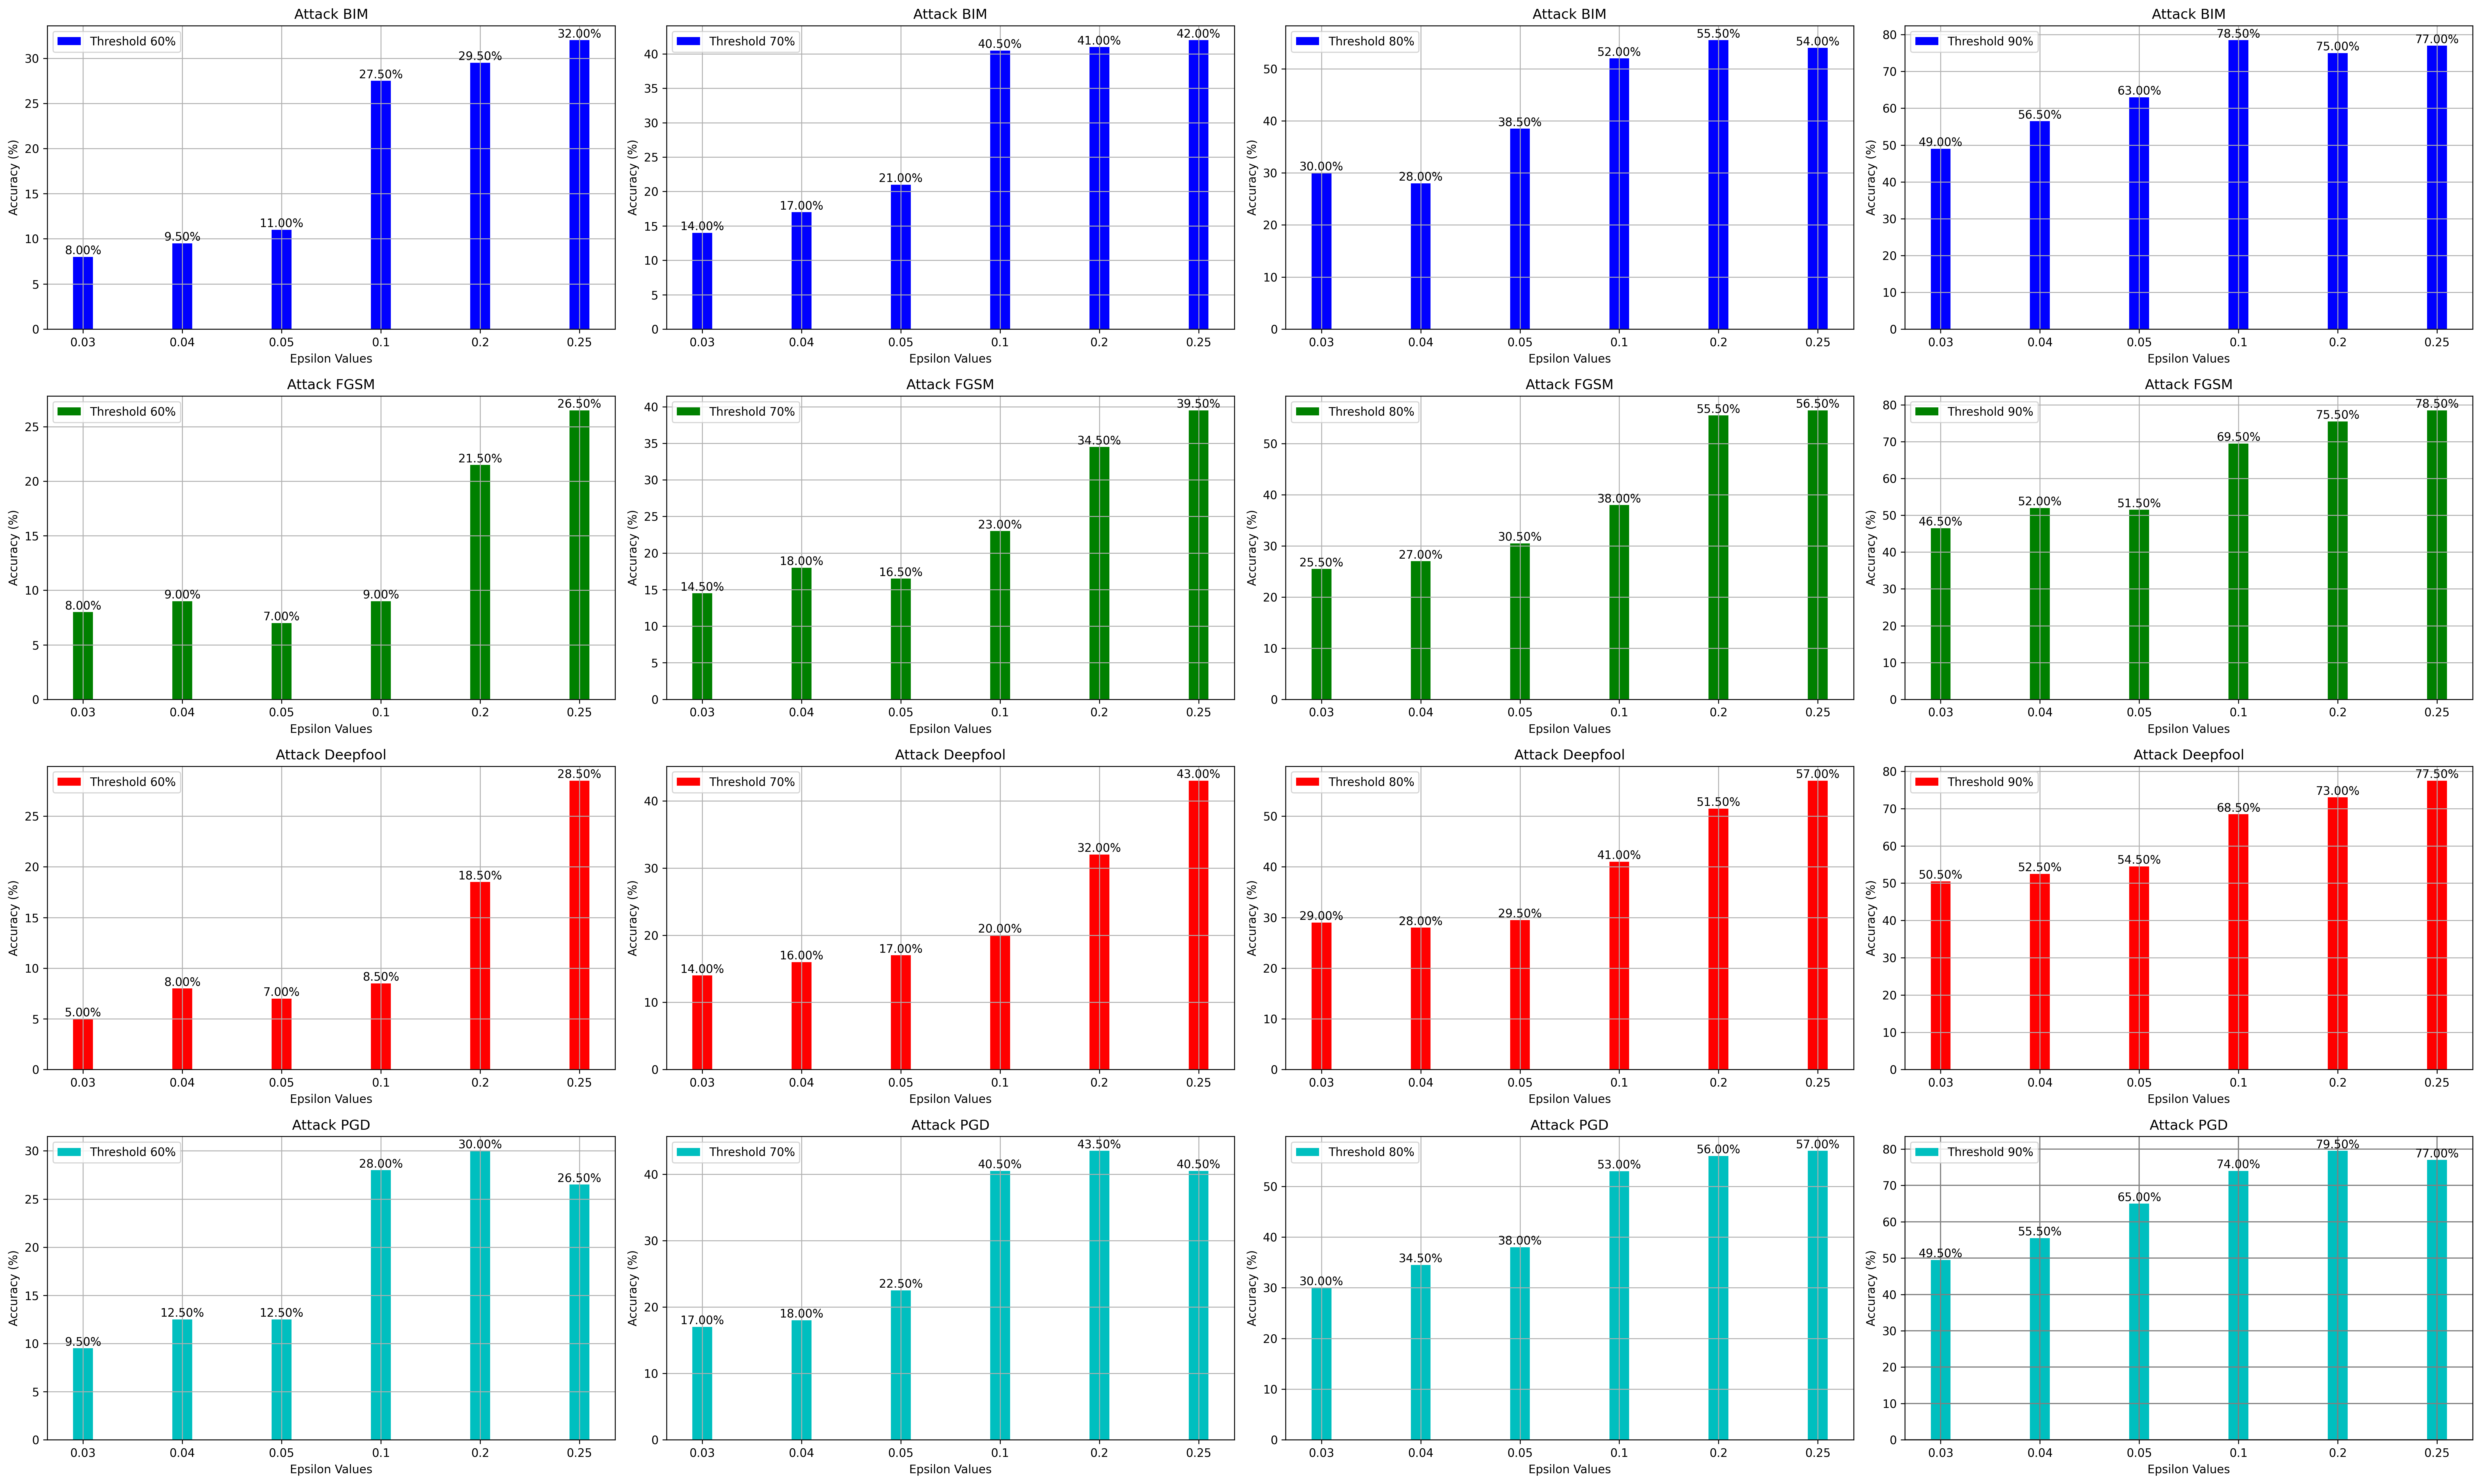
\includegraphics[width=\linewidth]{paper_images/correct absolute threshold.png}
%     \caption{correct absolute threshold}
%     \label{fig:fgsm_c}
% \end{figure*}
% \par\medskip % Adds space between the two subfigures
% \begin{figure*}
%     \centering
%     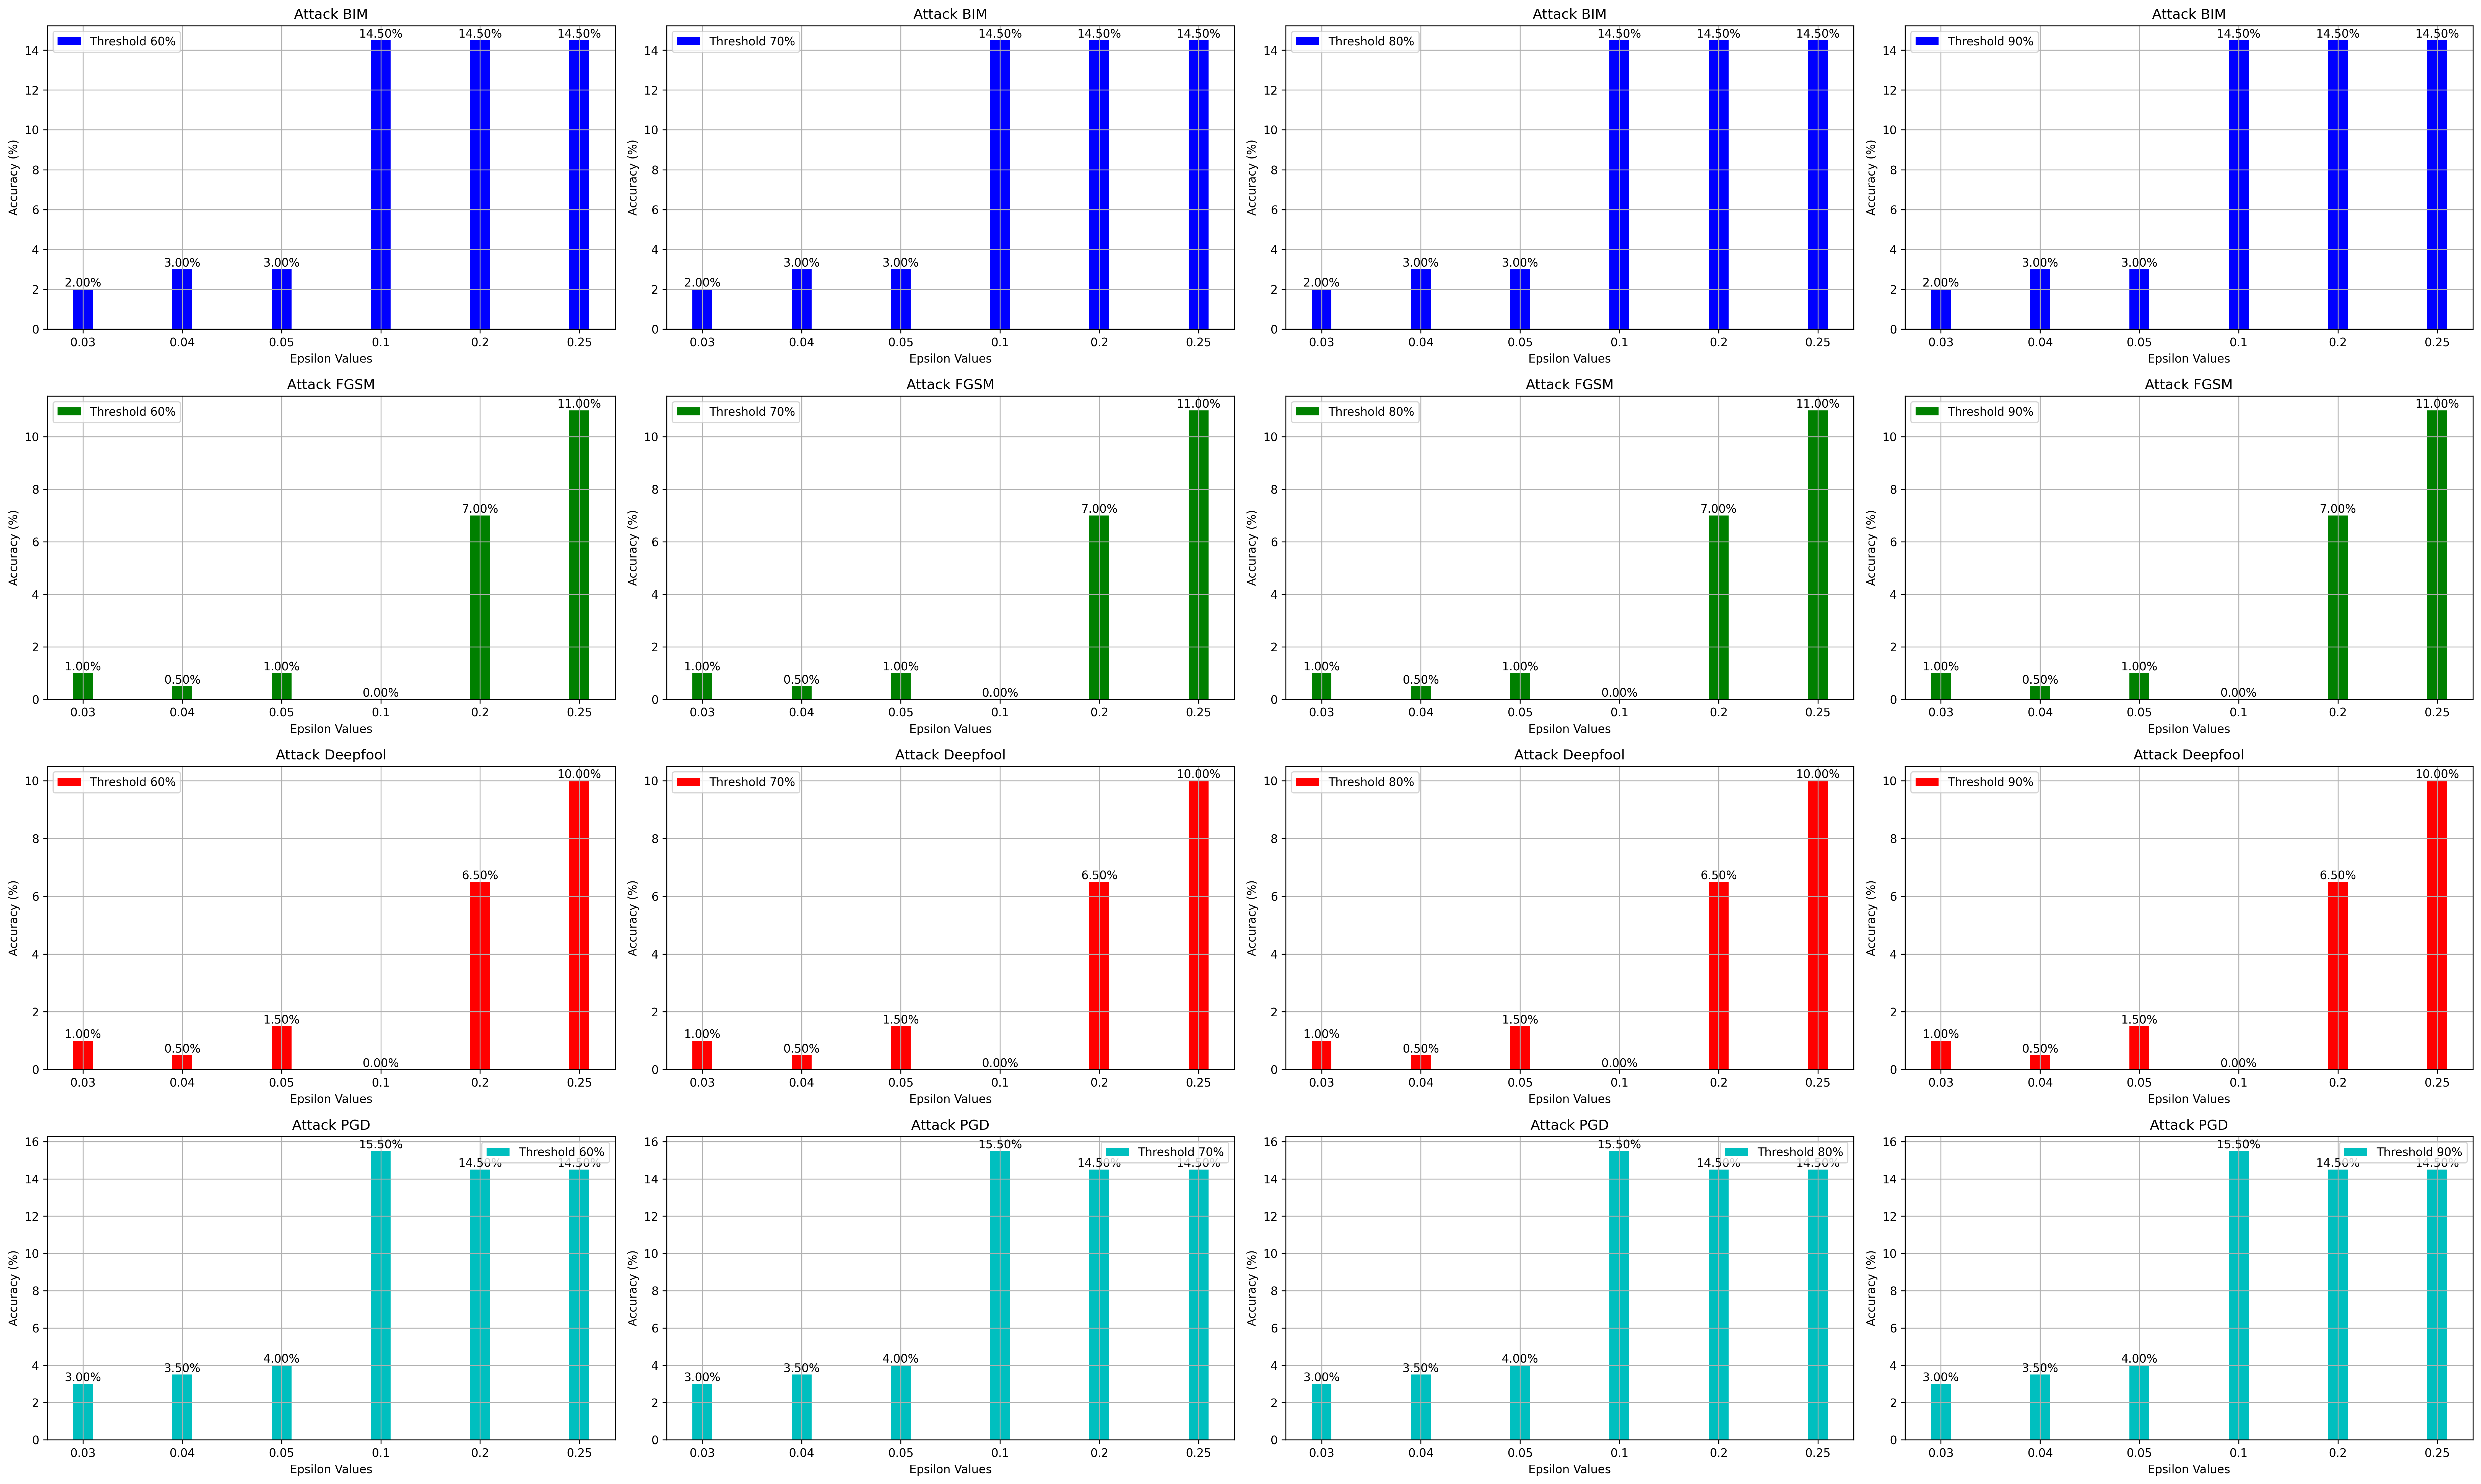
\includegraphics[width=\linewidth]{paper_images/correct negatice threshold.png}
%     \caption{correct negatice threshold}
%     \label{fig:deep_c}
% \end{figure*}
% \begin{figure*}
%     \centering
%     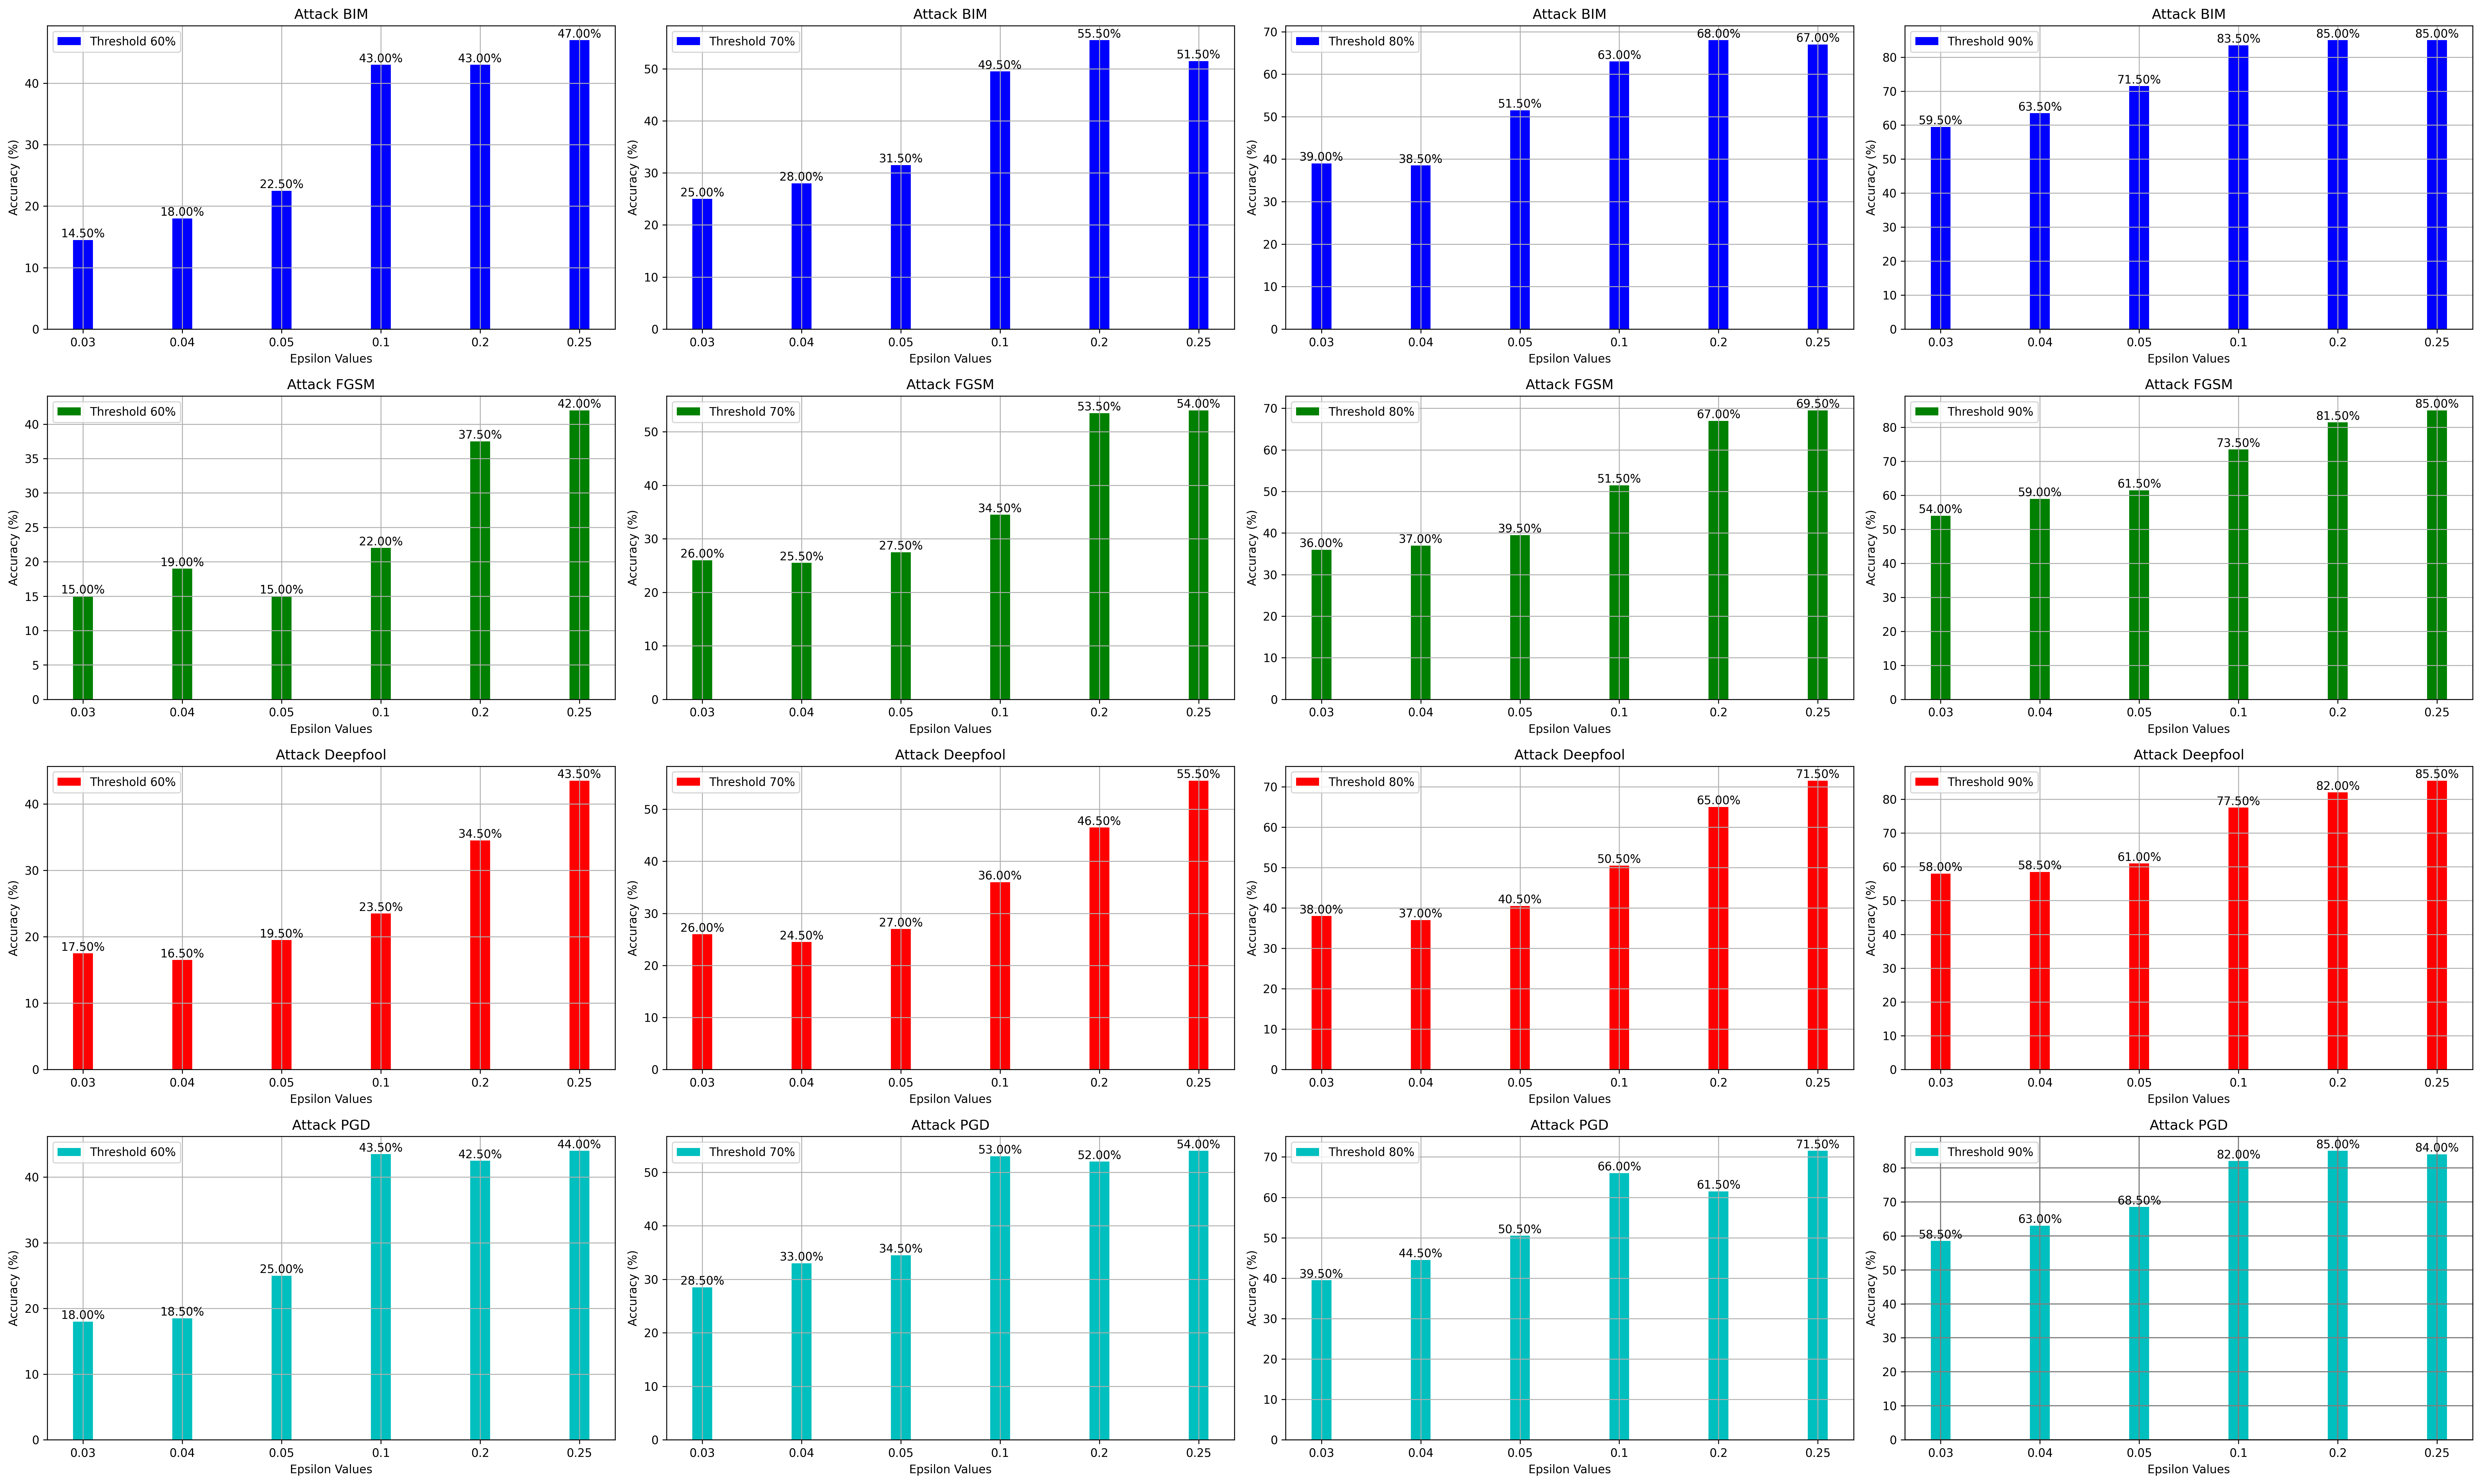
\includegraphics[width=\linewidth]{paper_images/correct positive threshold.png}
%     \caption{correct positive threshold}
%     \label{fig:fgsm}
% \end{figure*}




% \begin{figure*}
%     \centering
%     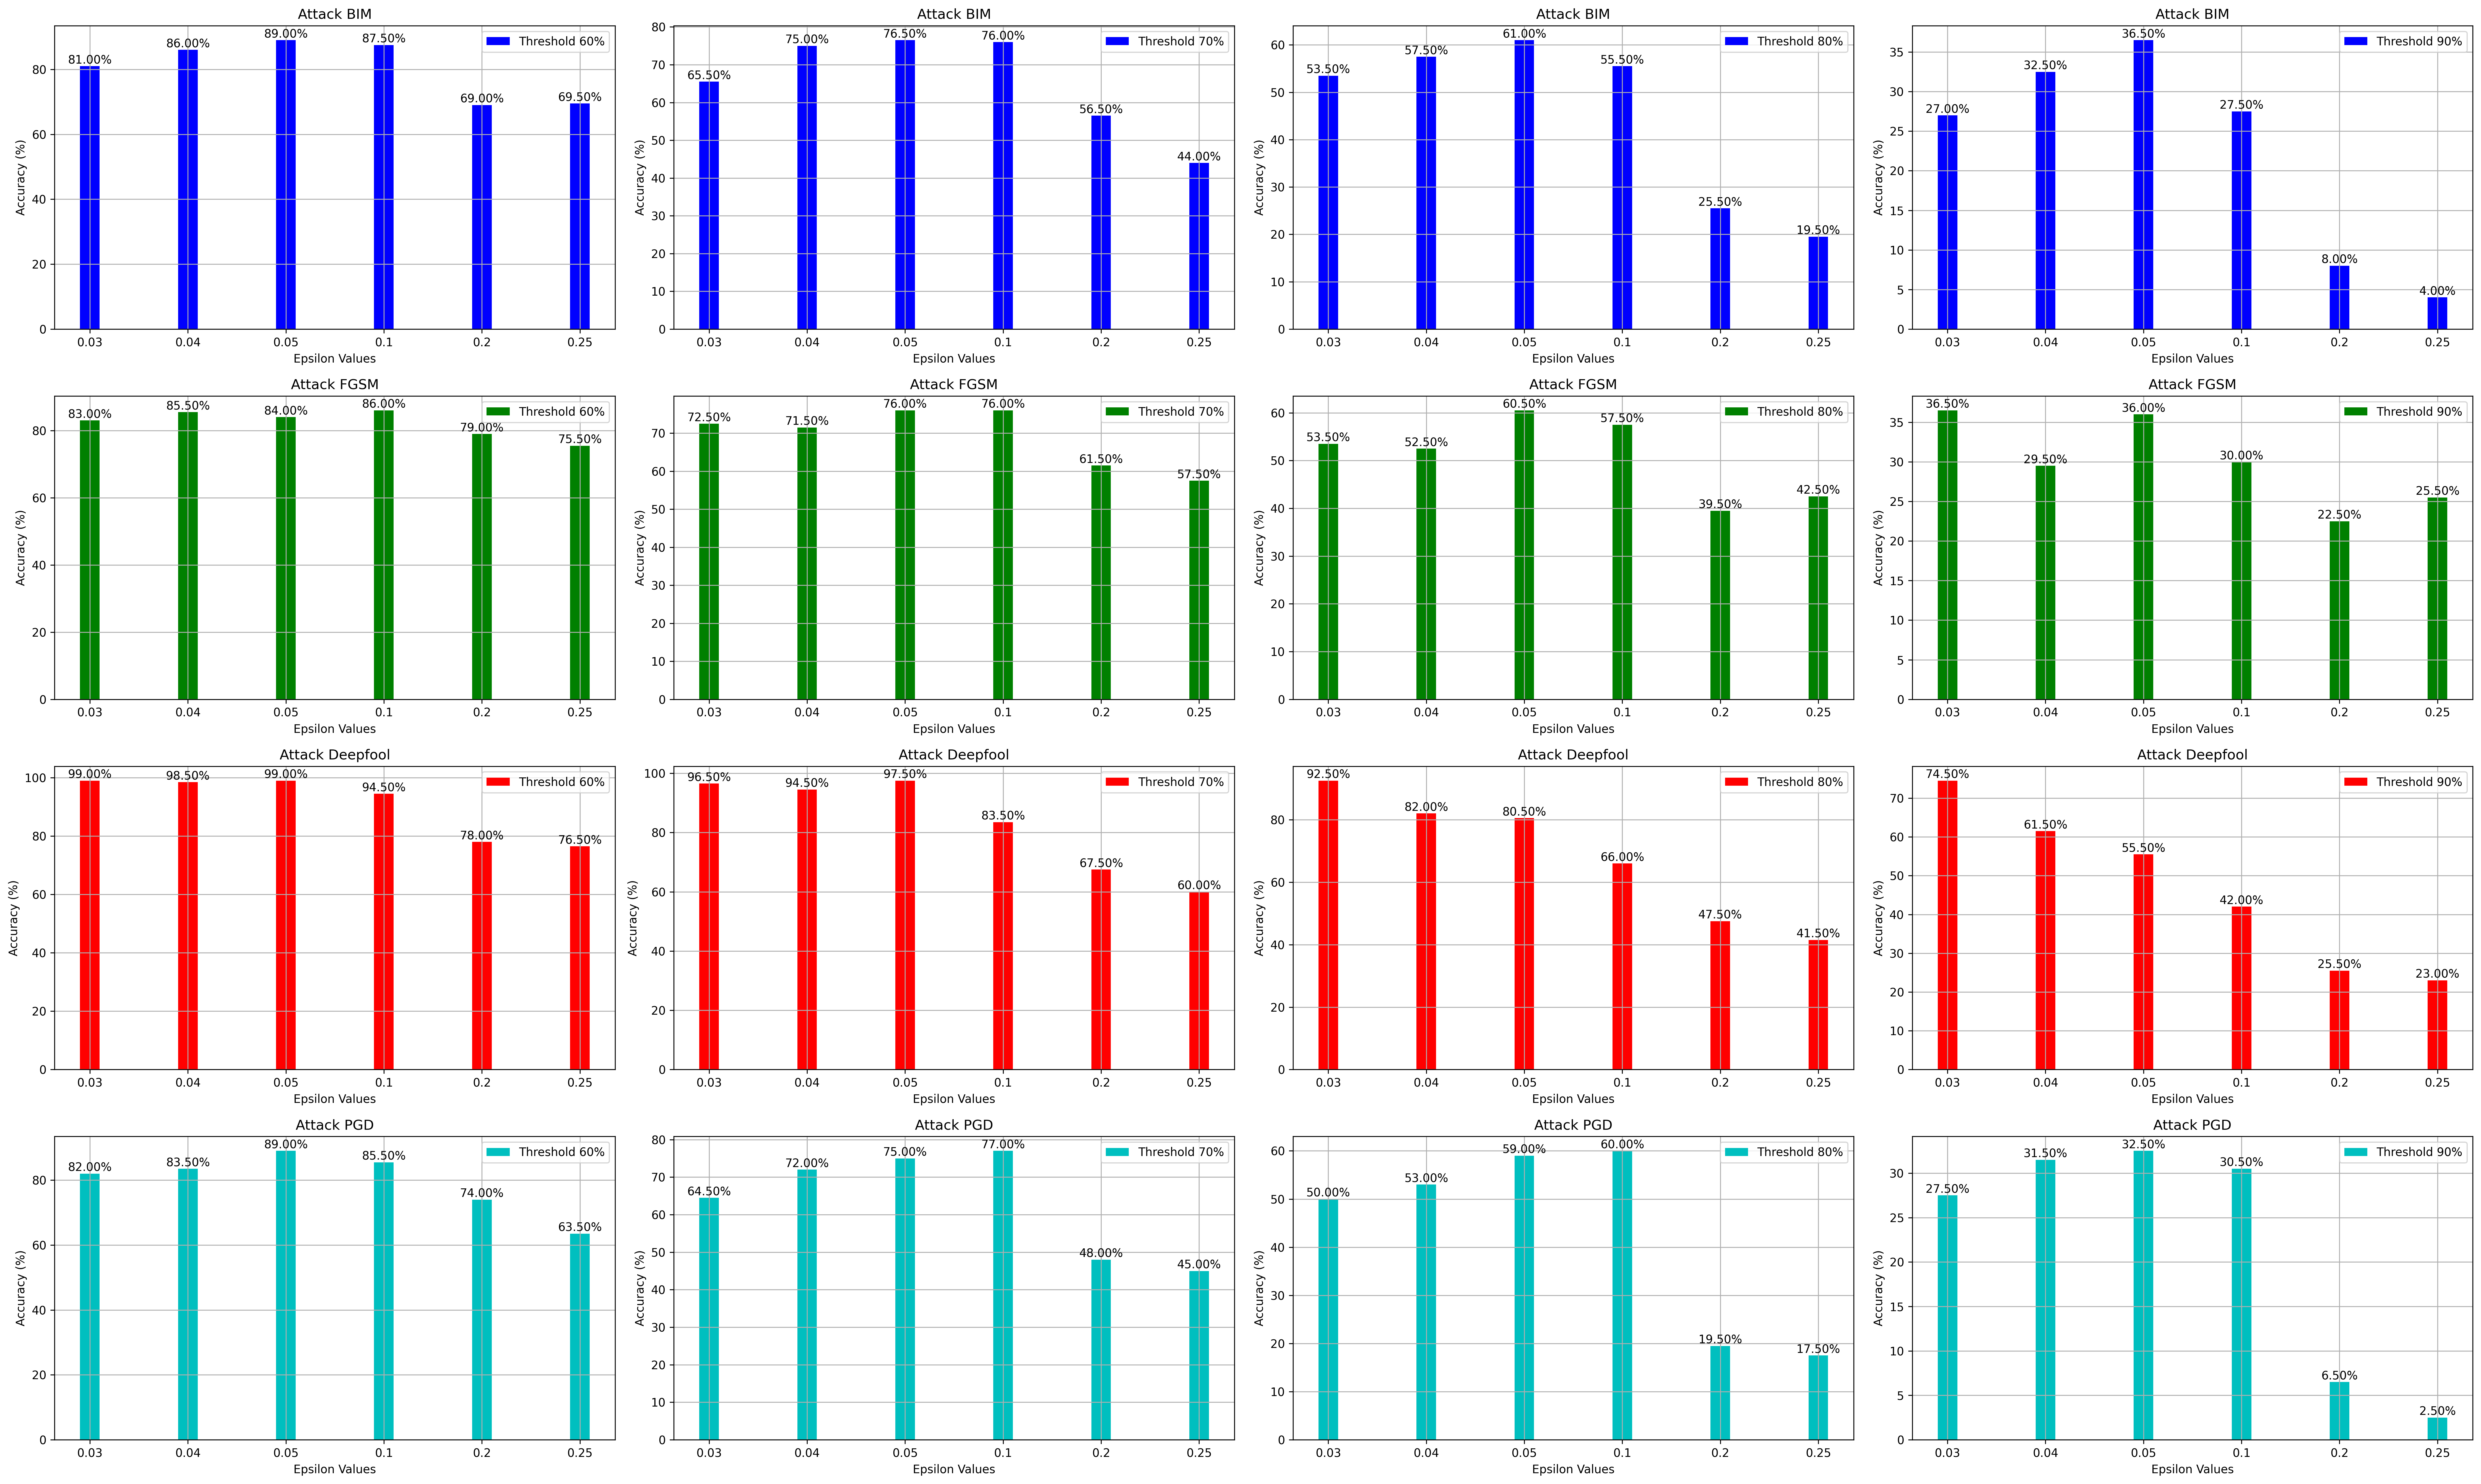
\includegraphics[width=\linewidth]{paper_images/aadversarial absolute threshold.png}
%     \caption{absolute adversarial threshold}
%     \label{fig:deep}
% \end{figure*}
% \begin{figure*}
%     \centering
%     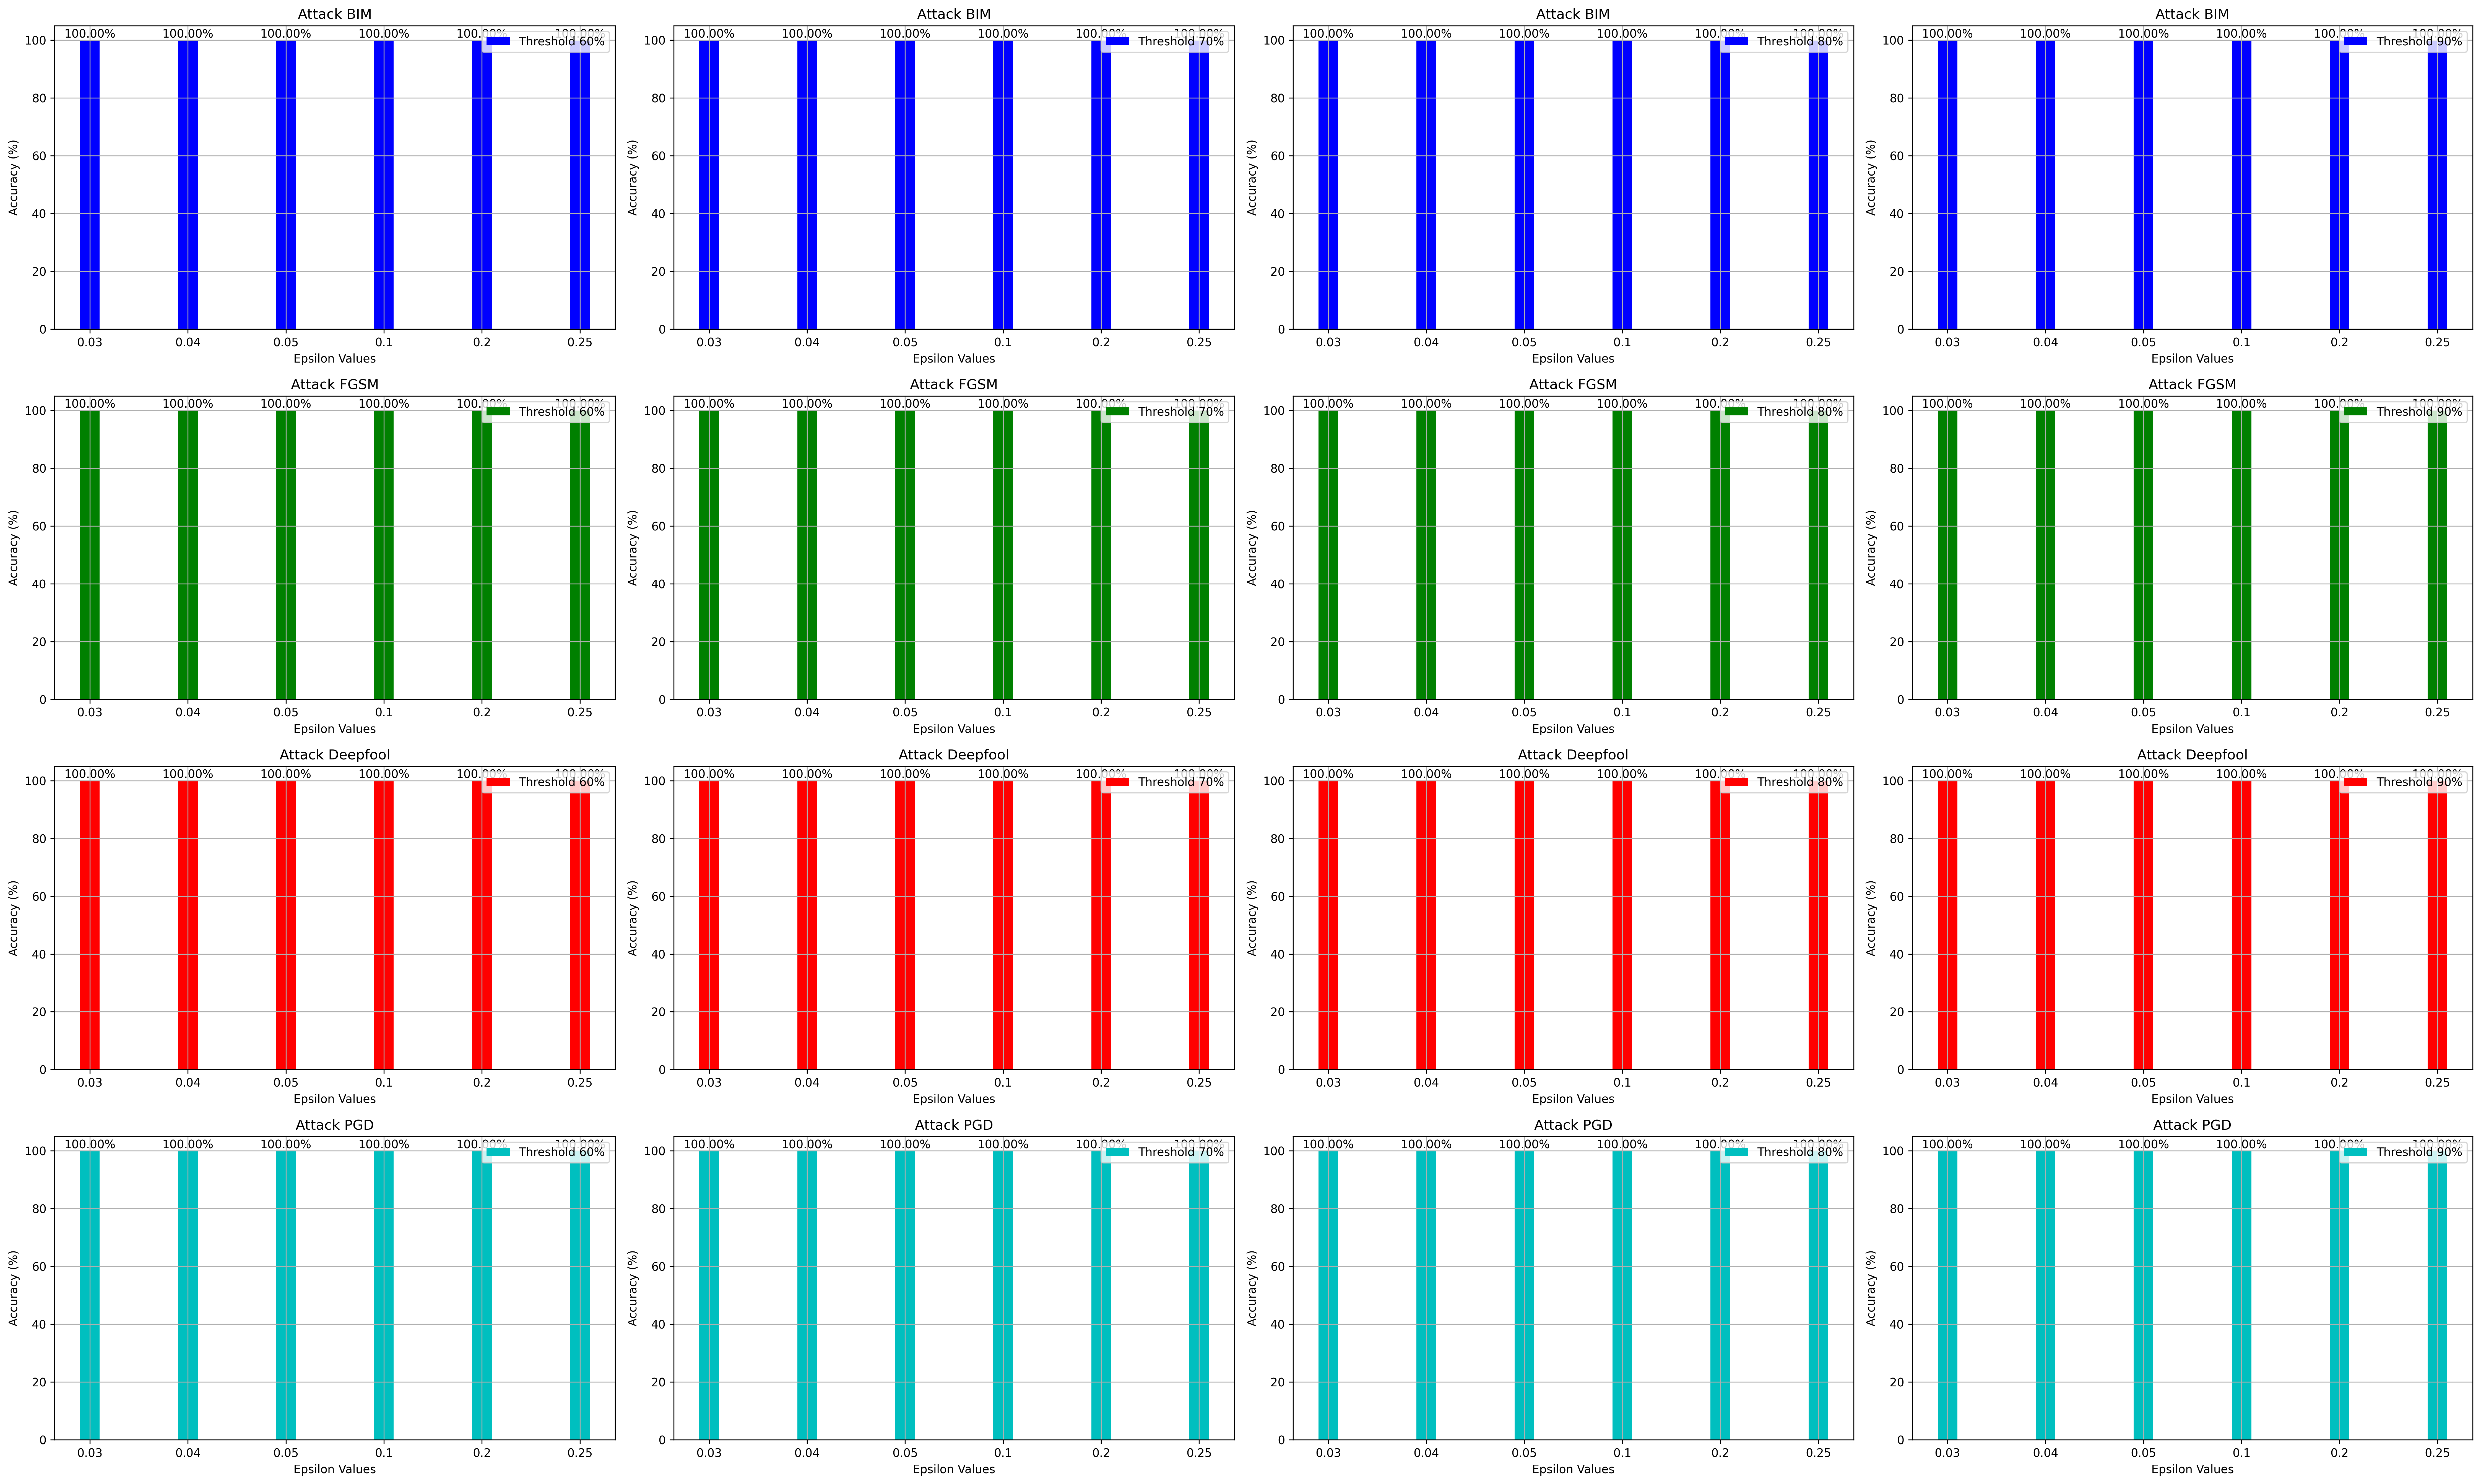
\includegraphics[width=\linewidth]{paper_images/negative adversarial threshold.png}
%     \caption{negative adversarial threshold}
%     \label{fig:deep}
% \end{figure*}
% \begin{figure*}
%     \centering
%     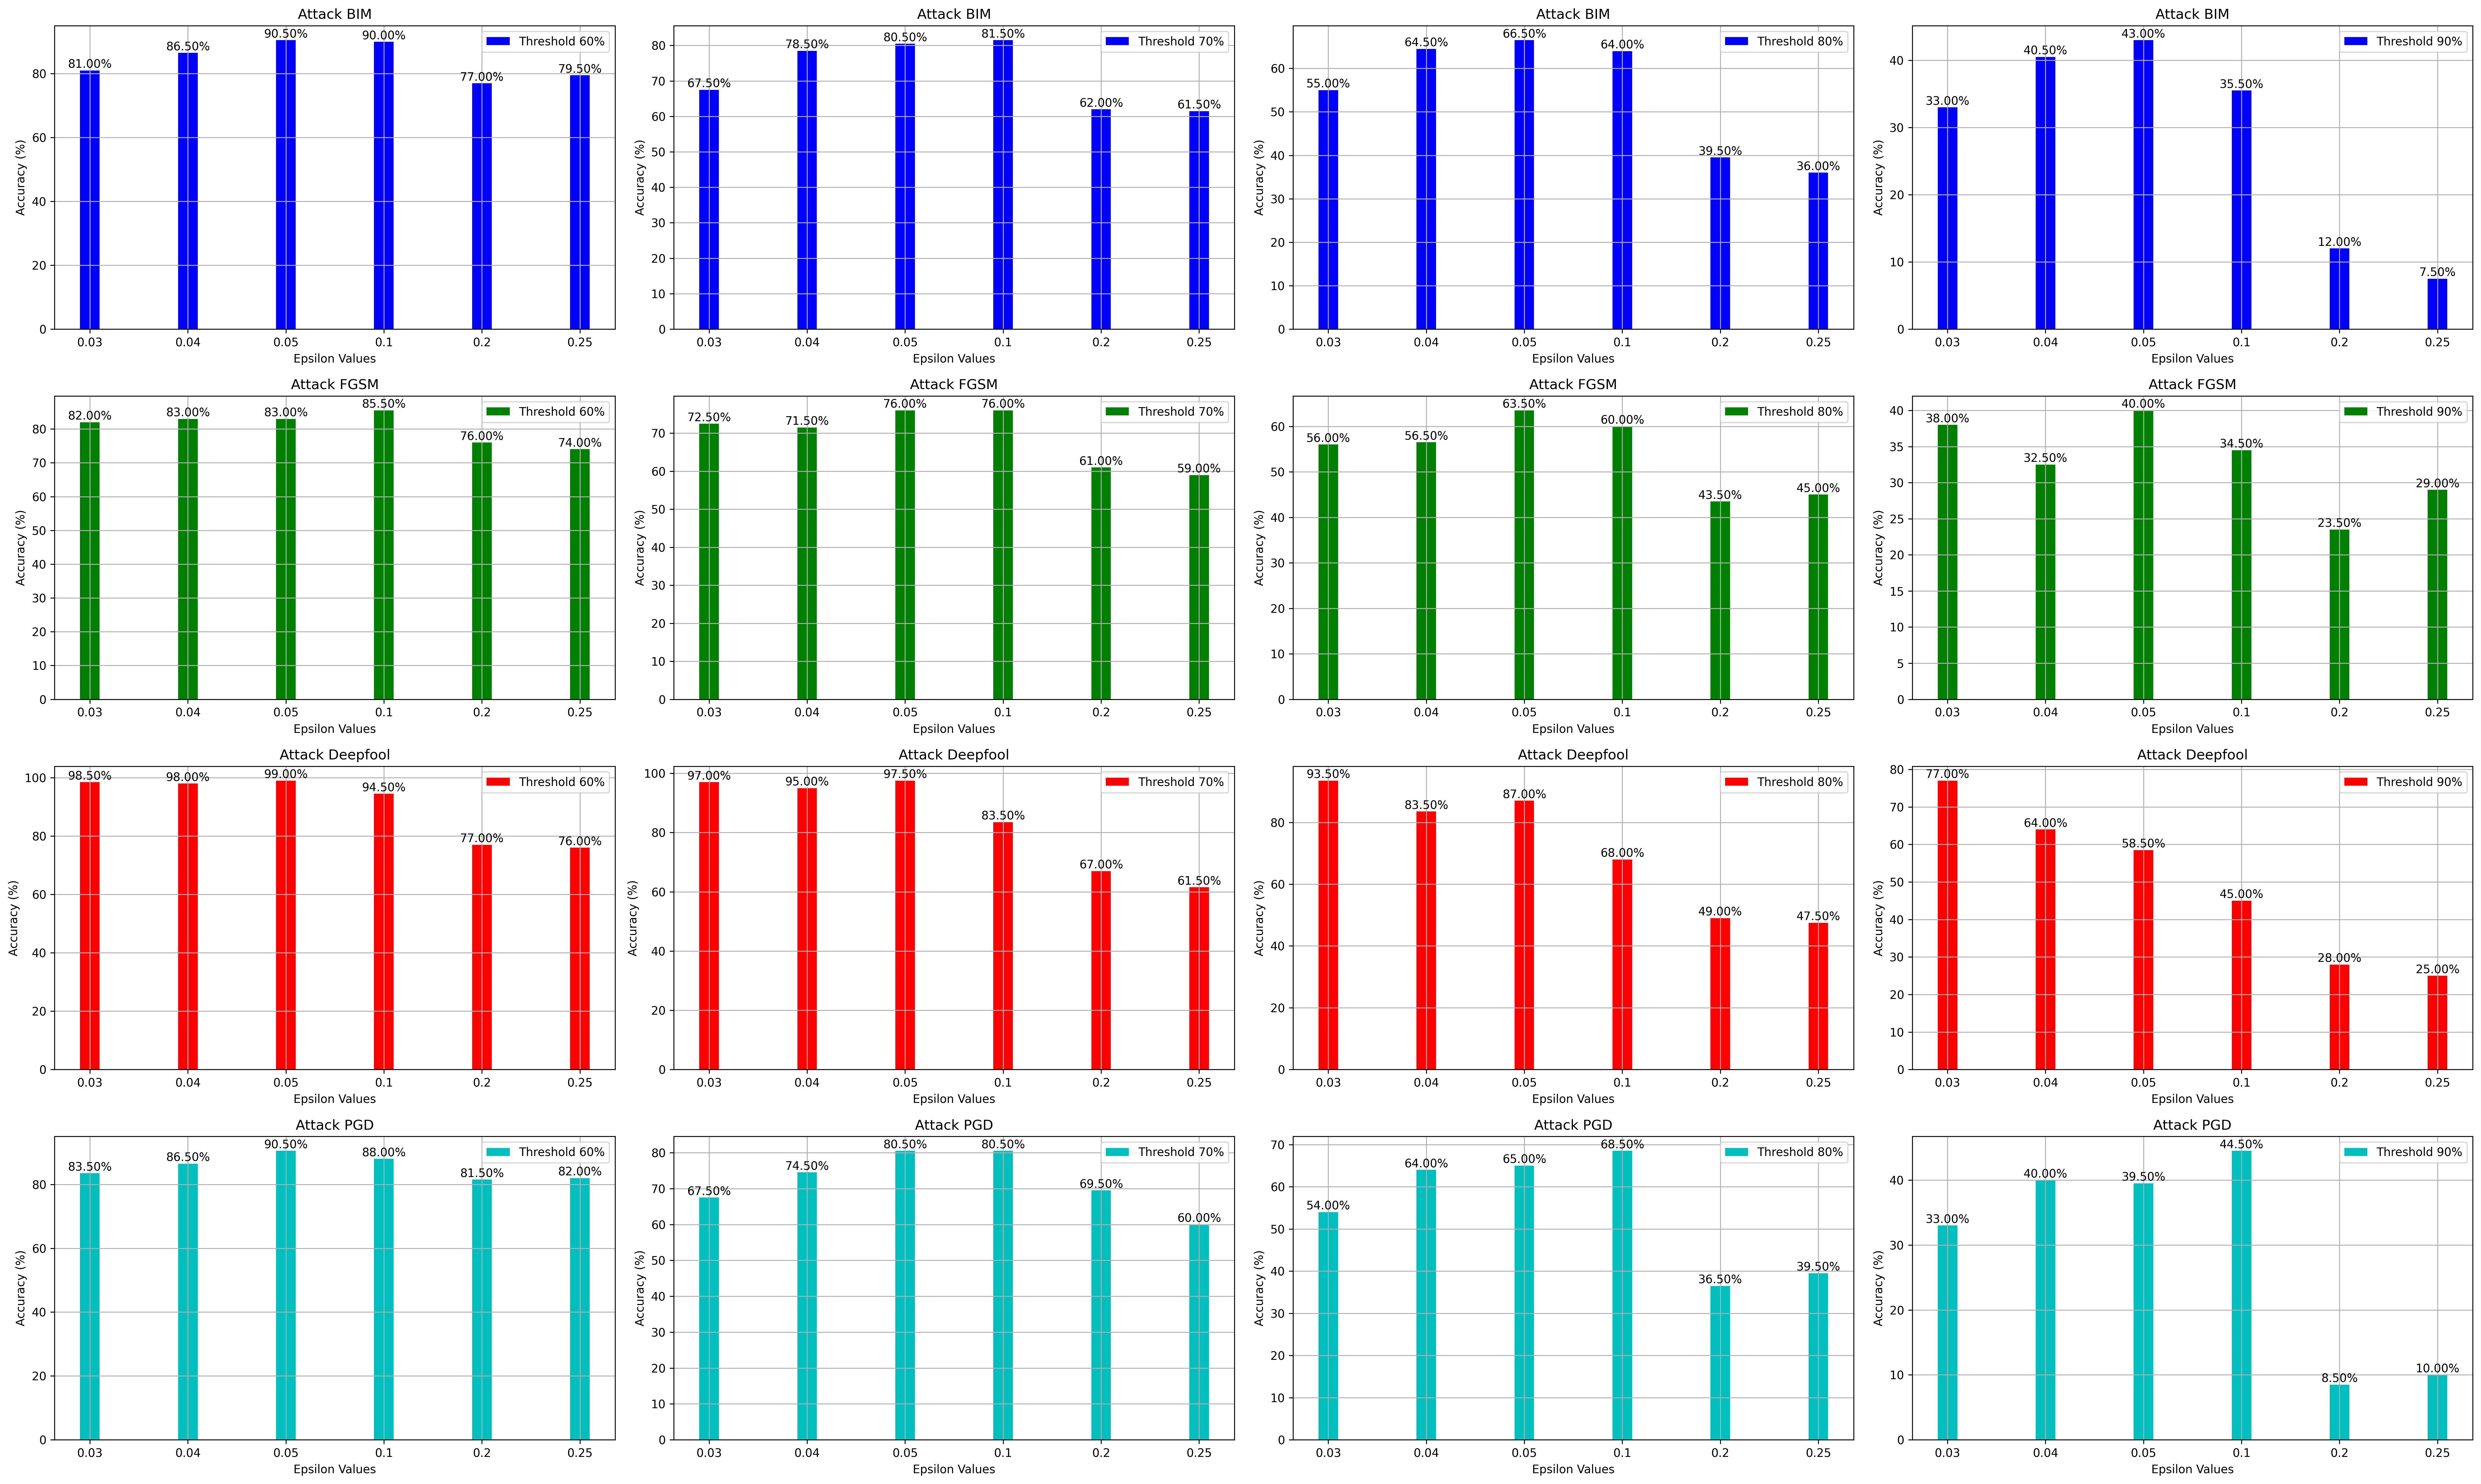
\includegraphics[width=\linewidth]{paper_images/positve adversarial threshold.png}
%     \caption{positve adversarial threshold}
%     \label{fig:deep}
% \end{figure*}

\end{document}
